% !TEX TS-program = lualatex
% =============================================================================
% ATP "Risco de Suicidio: avaliacao e conduta"
% Modulo E3M40, Funcionalidade III, Cognicao e Humor
% Medicina | Centro Universitario Campo Real | 2026
% Prof. Joao Frederico Musial
%
% Compilar: lualatex main.tex  (duas passadas)
%
% Este arquivo NAO contem nenhum frame. Preambulo e \input, apenas.
% Prelecao: 40 frames efetivos, partes 0 a 7.
% Transicao para a atividade: 2 frames, arquivo 08.
% =============================================================================
\PassOptionsToPackage{table}{xcolor}
\documentclass[aspectratio=43, handout]{beamer}

% =============================================================================
% preamble.tex
% ATP "Risco de Suicidio: avaliacao e conduta"
% Modulo E3M40, Funcionalidade III, Cognicao e Humor
% Medicina | Centro Universitario Campo Real | 2026
% Prof. Joao Frederico Musial
%
% Compilar com LuaLaTeX, duas passadas.
% =============================================================================

% --- Tema e cores institucionais --------------------------------------------
\usetheme{Madrid}
\makeatletter%%%%%%%%%%%%%%%%%%%%%%%%%%%%%%%%%%%%%%%%%%%%%%%%%%%%%%%%%%%%%%%%%%%%%%%%%%%%%%%
% beamercolorthemecamporeal.sty
% Cores institucionais e paletas do Beamer, Centro Universitario Campo Real.
%
% Herdado da serie Campo Real, com DUAS correcoes deliberadas em relacao ao
% arquivo que veio no projeto da fibromialgia, registradas aqui porque mudam a
% leitura de todo o material:
%
%   1. campoazul estava em RGB(68,0,102), que e roxo, e voltou ao azul
%      institucional RGB(0,51,102). O mapa de cor desta ATP reserva o azul para
%      avaliacao e entrevista, e o roxo para farmacologia; com o valor anterior
%      as duas familias colidiam.
%   2. campografite estava em RGB(0,102,0), que e verde, e passou a cinza
%      escuro real, RGB(58,63,69). O grafite carrega normativa, documento e
%      registro; com o valor anterior confundia-se com o verde de suporte e
%      continuidade.
%
% Preservados sem alteracao: campoamarelo, campoverde, campobordo, camporoxo.
%%%%%%%%%%%%%%%%%%%%%%%%%%%%%%%%%%%%%%%%%%%%%%%%%%%%%%%%%%%%%%%%%%%%%%%%%%%%%%%
\mode<presentation>

% --- CORES INSTITUCIONAIS ---------------------------------------------------
\definecolor{campoazul}{RGB}{0, 51, 102}      % Azul institucional
\definecolor{campoamarelo}{RGB}{255, 215, 0}  % Dourado institucional
\definecolor{campoverde}{RGB}{27, 138, 90}    % Verde de suporte e continuidade
\definecolor{campobordo}{RGB}{122, 0, 25}     % Vermelho queimado, acao imediata
\definecolor{camporoxo}{RGB}{102, 45, 145}    % Roxo, farmacologia

% --- CORES AUXILIARES -------------------------------------------------------
\definecolor{campoambar}{RGB}{191, 122, 0}    % Ambar, mudanca recente
\definecolor{campografite}{RGB}{58, 63, 69}   % Grafite, norma e registro
\definecolor{campoclaro}{RGB}{247, 247, 247}  % Fundo claro

% --- PALETA BEAMER ----------------------------------------------------------
\setbeamercolor{palette primary}{bg=campoazul, fg=white}
\setbeamercolor{palette secondary}{bg=campoamarelo!85, fg=black}
\setbeamercolor{palette tertiary}{bg=campoazul!90, fg=white}
\setbeamercolor{palette quaternary}{bg=campoazul!40, fg=white}

% --- TITULO DO FRAME --------------------------------------------------------
\setbeamercolor{frametitle}{bg=campoazul, fg=white}
\setbeamercolor{framesubtitle}{bg=campoazul, fg=white}

% --- CORPO ------------------------------------------------------------------
\setbeamercolor{structure}{fg=campoazul}
\setbeamercolor{normal text}{bg=white, fg=black}
\setbeamercolor{alerted text}{fg=campobordo}

% --- BLOCOS PADRAO ----------------------------------------------------------
\setbeamercolor{block title}{bg=campoazul!88, fg=white}
\setbeamercolor{block body}{bg=campoazul!8, fg=black}
\setbeamercolor{block title alerted}{bg=campobordo, fg=white}
\setbeamercolor{block body alerted}{bg=campobordo!7, fg=black}
\setbeamercolor{block title example}{bg=campoverde, fg=white}
\setbeamercolor{block body example}{bg=campoverde!8, fg=black}

% --- OUTROS ELEMENTOS -------------------------------------------------------
\setbeamercolor{title}{fg=campoazul, bg=white}
\setbeamercolor{author}{fg=campoazul!80!black, bg=white}
\setbeamercolor{institute}{fg=campografite, bg=white}
\setbeamercolor{date}{fg=campografite, bg=white}
\setbeamercolor{item}{fg=campoazul}
\setbeamercolor{caption name}{fg=campografite}

\mode<all>
\makeatother
\setbeamertemplate{navigation symbols}{}

% --- Pacotes essenciais -----------------------------------------------------
\usepackage{fontspec}
\IfFileExists{portuges.ldf}{\usepackage[brazil]{babel}}{\usepackage[english]{babel}}
\usepackage{csquotes}
\usepackage{graphicx}
\usepackage{amsmath,amssymb}
\usepackage{textcomp}
\usepackage{microtype}
\usepackage{setspace}
\usepackage{xfp}

% --- Icones -----------------------------------------------------------------
\usepackage{fontawesome5}

% --- Layout e tabelas -------------------------------------------------------
\usepackage{xcolor}
\usepackage{booktabs}
\usepackage{tabularx}
\usepackage{array}
\usepackage{multicol}

% --- Caixas e diagramas -----------------------------------------------------
\usepackage[most]{tcolorbox}
\usepackage{tikz}
\usepackage{pgfplots}
\pgfplotsset{compat=1.18}
\usetikzlibrary{arrows.meta, positioning, calc, fit, shapes.geometric,
                shapes.misc, shapes.symbols, matrix, backgrounds, chains,
                decorations.pathreplacing, patterns, shadows.blur}

% --- Acabamento editorial ----------------------------------------------------
% Regra da serie: o arredondamento e a sombra dos blocos vivem AQUI, no
% preambulo, e nunca em tema/boxes.tex.
\setbeamertemplate{blocks}[rounded][shadow=true]

% --- Tipografia --------------------------------------------------------------
% Duas familias, nenhuma terceira. Libertinus Serif no corpo, Roboto nos
% titulos curtos e nos marcadores. FontAwesome5 entra como icone, nao como
% familia de texto.
\setmainfont{Libertinus Serif}[
  UprightFont = LibertinusSerif-Regular,
  ItalicFont  = LibertinusSerif-Italic,
  BoldFont    = LibertinusSerif-Bold,
  BoldItalicFont = LibertinusSerif-BoldItalic,
  Extension = .otf ]
\setsansfont{Roboto}[
  UprightFont = Roboto-Regular,
  ItalicFont  = Roboto-Italic,
  BoldFont    = Roboto-Bold,
  BoldItalicFont = Roboto-BoldItalic,
  Extension = .ttf ]
\usefonttheme{serif}
\setbeamerfont{frametitle}{family=\sffamily, size=\large, series=\bfseries}
\setbeamerfont{framesubtitle}{family=\sffamily, size=\footnotesize}
\setbeamerfont{block title}{family=\sffamily, size=\small, series=\bfseries}
\setbeamerfont{block body}{size=\small}
\setbeamerfont{title}{family=\sffamily, series=\bfseries}
\setbeamerfont{author}{family=\sffamily}
\setbeamerfont{institute}{family=\sffamily}
\setbeamerfont{date}{family=\sffamily}
\setbeamertemplate{itemize items}[circle]
\setbeamertemplate{itemize subitem}[triangle]
\setlength{\parskip}{0pt}

% --- Margens internas do slide ----------------------------------------------
\setbeamersize{text margin left=0.45cm, text margin right=0.45cm}

% =============================================================================
% \CRar{k} : o botao unico de ar vertical do frame.
% -----------------------------------------------------------------------------
% k e adimensional. k = 0 e o piso em que nada estoura. De k derivam, de uma
% so vez, a distancia entre caixas, o respiro interno, a entrelinha do corpo,
% a separacao de itens de lista e a altura de linha de tabela. Como o frame do
% Beamer e um grupo TeX, cada frame escreve o seu proprio k em UMA linha, no
% proprio arquivo. Nunca aplicar o mesmo incremento a todas as paginas: a folga
% varia de pagina para pagina.
% =============================================================================
\newlength{\CRgapbox}      % distancia entre caixas
\newlength{\CRitemsep}     % separacao entre itens de lista
\newlength{\CRestica}      % meia altura da regua invisivel das tabelas
\newlength{\CRcolentidade} % largura fixa da primeira coluna de tabela
\setlength{\CRcolentidade}{2.55cm}

\newcommand{\CRar}[1]{%
  \setlength{\CRgapbox}{\fpeval{0.12 + 0.115*(#1)}cm}%
  \setlength{\CRitemsep}{\fpeval{0.15 + 0.28*(#1)}ex}%
  \setlength{\CRestica}{\fpeval{0.55 + 0.30*(#1)}ex}%
  \renewcommand{\baselinestretch}{\fpeval{1.00 + 0.030*(#1)}}%
  \selectfont
}
\CRar{0}

% Espaco vertical entre caixas, sempre pelo botao.
\newcommand{\CRvg}{\vspace{\CRgapbox}}

% --- Camadas do tema ---------------------------------------------------------
% =============================================================================
% tema/boxes.tex - caixas semanticas, ferramentas de tabela e macros de autor
% -----------------------------------------------------------------------------
% Decisao herdada da serie: as caixas de conteudo sao construidas sobre o block
% nativo do Beamer, nao sobre tcolorbox, para que raio de canto, respiro interno
% e tipografia de titulo sejam os mesmos em toda a serie. O arredondamento e a
% sombra estao no preambulo, com \setbeamertemplate{blocks}[rounded][shadow],
% e nao aqui.
%
% \CRnewblock tem QUATRO argumentos. O marcador de itemizacao herda a cor pela
% definicao de "local structure" e "item" com a cor do TITULO da caixa.
% =============================================================================

% #1 nome do ambiente | #2 cor do titulo | #3 cor do fundo | #4 cor do texto do titulo
\newcommand{\CRnewblock}[4]{%
  \newenvironment{#1}[1]{%
    \begingroup
    \setbeamercolor{block title}{bg=#2, fg=#4}%
    \setbeamercolor{block body}{bg=#3, fg=black}%
    \setbeamercolor{local structure}{fg=#2}%
    \setbeamercolor{item}{fg=#2}%
    \begin{block}{##1}%
  }{%
    \end{block}%
    \endgroup
  }%
}

% =============================================================================
% AS SEIS CAIXAS. Uma por funcao do mapa de cor do briefing. Nenhuma outra cor.
%   azul     avaliacao e entrevista
%   ambar    mudanca recente e janelas de vigilancia
%   bordo    acao imediata, disposicao, remocao, ambiente protegido
%   verde    suporte, protecao, plano de seguranca, continuidade
%   grafite  normativa, documento e registro
%   roxo     farmacologia
% =============================================================================
\CRnewblock{CRbaseavaliar}{campoazul!88}{campoazul!8}{white}
\CRnewblock{CRbasemudanca}{campoambar}{campoambar!10}{white}
\CRnewblock{CRbaseagir}{campobordo}{campobordo!7}{white}
\CRnewblock{CRbaseproteger}{campoverde}{campoverde!8}{white}
\CRnewblock{CRbasenorma}{campografite}{campografite!7}{white}
\CRnewblock{CRbasefarmaco}{camporoxo}{camporoxo!8}{white}

% =============================================================================
% VOCABULARIO DE ICONE
% -----------------------------------------------------------------------------
% Um icone por FUNCAO, sempre o mesmo, nunca outro. O icone nao decora: ele diz,
% antes da leitura, a que familia aquela caixa pertence, do mesmo modo que a cor.
% Cor e icone andam juntos e nenhum dos dois aparece sozinho.
%
% Todos os nomes usados aqui constam da Comprehensive LaTeX Symbol List e foram
% conferidos um a um contra a instalacao (ferramentas/simbolos.py).
% =============================================================================
\newcommand{\iAvaliar}{\faComments}          % avaliacao e entrevista
\newcommand{\iMudanca}{\faClock}             % mudanca recente e vigilancia
\newcommand{\iAgir}{\faAmbulance}            % acao imediata e disposicao
\newcommand{\iProteger}{\faHandsHelping}     % suporte, protecao, continuidade
\newcommand{\iNorma}{\faBalanceScale}        % normativa, documento, registro
\newcommand{\iFarmaco}{\faPills}             % farmacologia

% As seis caixas, cada uma ja com o seu icone no titulo.
\newenvironment{caixaavaliar}[1]{\begin{CRbaseavaliar}{\iAvaliar~~#1}}{\end{CRbaseavaliar}}
\newenvironment{caixamudanca}[1]{\begin{CRbasemudanca}{\iMudanca~~#1}}{\end{CRbasemudanca}}
\newenvironment{caixaagir}[1]{\begin{CRbaseagir}{\iAgir~~#1}}{\end{CRbaseagir}}
\newenvironment{caixaproteger}[1]{\begin{CRbaseproteger}{\iProteger~~#1}}{\end{CRbaseproteger}}
\newenvironment{caixanorma}[1]{\begin{CRbasenorma}{\iNorma~~#1}}{\end{CRbasenorma}}
\newenvironment{caixafarmaco}[1]{\begin{CRbasefarmaco}{\iFarmaco~~#1}}{\end{CRbasefarmaco}}

% Titulo de frame com icone de orientacao. O icone marca a etapa da cadeia
% avaliar, formular, decidir, construir seguranca, garantir continuidade, e
% permite ao aluno saber onde esta sem ler o titulo inteiro.
\newcommand{\ftit}[2]{#1\,\,#2}

% =============================================================================
% REALCES DE TEXTO
% =============================================================================
\newcommand{\avaliar}[1]{\textbf{\color{campoazul!90!black}#1}}
\newcommand{\mudanca}[1]{\textbf{\color{campoambar!90!black}#1}}
\newcommand{\agir}[1]{\textbf{\color{campobordo!90!black}#1}}
\newcommand{\proteger}[1]{\textbf{\color{campoverde!80!black}#1}}
\newcommand{\norma}[1]{\textbf{\color{campografite}#1}}
\newcommand{\farmaco}[1]{\textbf{\color{camporoxo!88!black}#1}}

% Fala literal a ser dita ao paciente ou a familia. Vai para a tela como esta.
\newcommand{\fala}[1]{{\itshape\color{campoazul!85!black}\guillemotleft #1\guillemotright}}

% Procedencia discreta, ao pe do frame.
\newcommand{\fonte}[1]{%
  \par\vspace{0.4ex}%
  {\raggedleft\scriptsize\sffamily\color{campografite}#1\par}%
}

% Rotulo curto embutido no texto.
\newcommand{\chip}[2]{%
  \tikz[baseline=(x.base)]{\node[chipno={#1}] (x) {\strut #2};}%
}

% Grau de vinculacao da afirmacao. A aula separa o que e norma, o que e
% interpretacao clinica e o que e recomendacao apoiada em evidencia.
\newcommand{\selonorma}{{\scriptsize\sffamily\color{campografite}\textbf{[norma]}}}
\newcommand{\seloevidencia}{{\scriptsize\sffamily\color{campoverde}\textbf{[evid\^encia]}}}
\newcommand{\seloclinico}{{\scriptsize\sffamily\color{campoazul}\textbf{[interpreta\c{c}\~ao cl\'inica]}}}

% =============================================================================
% MENSAGEM DOMINANTE DO FRAME
% Largura total. Nunca dentro de columns.
% =============================================================================
\newcommand{\mensagem}[1]{%
  \par\vspace{\CRgapbox}%
  \begingroup
  \setlength{\fboxsep}{5pt}%
  \noindent\colorbox{campoazul!10}{%
    \parbox{\dimexpr\textwidth-2\fboxsep\relax}{%
      \centering\small\sffamily\bfseries\color{campoazul!90!black}#1}}%
  \endgroup
  \par
}
\newcommand{\mensagemagir}[1]{%
  \par\vspace{\CRgapbox}%
  \begingroup
  \setlength{\fboxsep}{5pt}%
  \noindent\colorbox{campobordo!8}{%
    \parbox{\dimexpr\textwidth-2\fboxsep\relax}{%
      \centering\small\sffamily\bfseries\color{campobordo}#1}}%
  \endgroup
  \par
}

% =============================================================================
% ITENS COMPACTOS, com a separacao governada pelo botao de ar
% =============================================================================
\newenvironment{itemc}{%
  \begin{itemize}\setlength{\itemsep}{\CRitemsep}\setlength{\parskip}{0pt}%
  \setlength{\topsep}{0pt}\setlength{\partopsep}{0pt}%
}{%
  \end{itemize}%
}

% Calha explicita entre colunas. Nenhum par de colunas soma mais de 0.94.
\newcommand{\calha}{\hspace{0.035\textwidth}}

% =============================================================================
% TABELAS DA SERIE
% -----------------------------------------------------------------------------
% A altura de linha vem de uma regua invisivel IDENTICA no inicio de TODA
% celula, governada por \CRestica, e nunca de \extrarowheight, que acrescenta
% espaco so acima da linha de base e desalinha o rotulo da primeira coluna.
% A primeira coluna e coluna de paragrafo de largura fixa, tipo E, e nunca l.
% Dentro do ambiente vale \lefthyphenmin=3. A barra de celula se escreve
% \slash, que imprime a mesma barra e admite quebra depois dela.
% =============================================================================
\newcommand{\CRregua}{\rule[-\CRestica]{0pt}{\dimexpr 2\CRestica + 1em\relax}}
\newcolumntype{E}{>{\CRregua\raggedright\arraybackslash}p{\CRcolentidade}}
\newcolumntype{P}[1]{>{\CRregua\raggedright\arraybackslash}p{#1}}
\newcolumntype{C}[1]{>{\CRregua\centering\arraybackslash}p{#1}}

\newenvironment{CRtabela}{%
  \begingroup
  \lefthyphenmin=3\relax
  \sffamily\footnotesize
  \setlength{\tabcolsep}{3pt}%
  \renewcommand{\arraystretch}{1.0}%
  \arrayrulecolor{campoazul!35}%
}{%
  \endgroup
}

% =============================================================================
% \quadroDx : macro UNICA dos frames da parte 3B. Geometria identica em todas
% as ocorrencias, dois quadros por frame. Nao revisa o diagnostico.
%   #1 quadro | #2 o que eleva o risco aqui | #3 o que muda na conduta
%   #4 erro classico
% =============================================================================
\newcommand{\quadroDx}[4]{%
  \begin{tcolorbox}[
      enhanced, sharp corners=downhill, arc=3pt, boxrule=0.9pt,
      colframe=campoazul!75!black, colback=white,
      left=5pt, right=5pt, top=4pt, bottom=4pt,
      width=\linewidth, height=6.15cm, valign=top,
      drop shadow={black!35},
      fontupper=\scriptsize,
      title={\sffamily\bfseries #1}, fonttitle=\scriptsize,
      colbacktitle=campoazul!88, coltitle=white,
      attach boxed title to top left={xshift=5pt, yshift=-2pt},
      boxed title style={sharp corners=downhill, arc=2pt, boxrule=0pt}]
    \vspace{0.26cm}
    {\sffamily\bfseries\scriptsize\color{campoambar!88!black}O QUE ELEVA O RISCO AQUI}\par
    \vspace{0.05cm}#2\par
    \vspace{0.17cm}
    {\sffamily\bfseries\scriptsize\color{campobordo}O QUE MUDA NA CONDUTA}\par
    \vspace{0.05cm}#3\par
    \vspace{0.17cm}
    {\sffamily\bfseries\scriptsize\color{campografite}ERRO CL\'ASSICO}\par
    \vspace{0.05cm}#4
  \end{tcolorbox}%
}

% =============================================================================
% tema/tikz.tex - vocabulario grafico da serie
% -----------------------------------------------------------------------------
% Conjunto musial*, herdado sem ruptura da implementacao de referencia
% (FIBROMIALGIA_2026_REFINADA): gradiente branco para tonalidade clara, borda
% semantica, sombra difusa discreta e seta com a cor do destino.
%
% Acrescimos validados na serie e mantidos aqui: supressao de hifenizacao em
% todo no, os atalhos crnode, crseta e passo, a moldura \bandaimg e o \chip.
%
% Regra que vale em todo frame: a seta sai de uma FACE explicita do no
% (.south, .east, .north, .west) e nunca do centro. Uma seta ancorada no centro
% calcula o ++ a partir do centro e, quando a altura minima do no cresce, o
% rotulo cai dentro da propria caixa.
% =============================================================================

\tikzset{
  % --- base -----------------------------------------------------------------
  musialBase/.style={rectangle, rounded corners=3pt, very thick, align=center,
                     inner xsep=6pt, inner ysep=5pt, font=\footnotesize,
                     execute at begin node={\hyphenpenalty=10000\exhyphenpenalty=10000},
                     blur shadow={shadow blur steps=4, shadow xshift=0.8pt,
                                  shadow yshift=-0.8pt}},
  musialBlue/.style={musialBase, draw=campoazul!80!black,
                     top color=white, bottom color=campoazul!18},
  musialGreen/.style={musialBase, draw=campoverde!82!black,
                      top color=white, bottom color=campoverde!18},
  musialRed/.style={musialBase, draw=campobordo!88!black,
                    top color=white, bottom color=campobordo!14},
  musialAmber/.style={musialBase, draw=campoambar!88!black,
                      top color=white, bottom color=campoambar!18},
  musialPurple/.style={musialBase, draw=camporoxo!80!black,
                       top color=white, bottom color=camporoxo!16},
  musialYellow/.style={musialBase, draw=campoamarelo!72!black,
                       top color=white, bottom color=campoamarelo!24},
  musialNeutral/.style={musialBase, draw=campografite!55,
                        top color=white, bottom color=campografite!6},
  % --- circulo central ------------------------------------------------------
  musialCenter/.style={circle, very thick, draw=campoazul!85!black,
                       top color=white, bottom color=campoazul!28,
                       text=campoazul!90!black, align=center,
                       font=\small\bfseries\sffamily,
                       minimum size=2.25cm, inner sep=4pt,
                       execute at begin node={\hyphenpenalty=10000\exhyphenpenalty=10000},
                       blur shadow={shadow blur steps=5, shadow xshift=1pt,
                                    shadow yshift=-1pt}},
  % --- setas ----------------------------------------------------------------
  musialFlow/.style={-{Latex[length=2.5mm,width=1.8mm]}, line width=0.8pt,
                     campoazul!85!black, rounded corners=4pt},
  musialFlowGreen/.style={musialFlow, campoverde!85!black},
  musialFlowRed/.style={musialFlow, campobordo!88!black},
  musialFlowAmber/.style={musialFlow, campoambar!90!black},
  musialFlowPurple/.style={musialFlow, camporoxo!85!black},
  musialFlowGraf/.style={musialFlow, campografite!80},
  musialThin/.style={-{Latex[length=2.0mm]}, semithick, campografite!70},
  musialBi/.style={{Latex[length=2.2mm,width=1.6mm]}-{Latex[length=2.2mm,width=1.6mm]},
                   line width=0.7pt, campoazul!75!black, rounded corners=4pt},
  % --- dose, herdados -------------------------------------------------------
  musialDose/.style={musialBlue, text width=3.0cm, minimum height=0.95cm,
                     font=\footnotesize},
  musialDoseTarget/.style={musialGreen, text width=3.0cm, minimum height=0.95cm,
                           font=\footnotesize},
  % --- rotulo sobre linha ---------------------------------------------------
  musialRot/.style={font=\scriptsize\sffamily, text=campografite,
                    fill=white, fill opacity=0.9, text opacity=1,
                    inner sep=1.6pt, rounded corners=1pt, align=center},
  % --- chip inline ----------------------------------------------------------
  chipno/.style args={#1}{rectangle, rounded corners=2pt, draw=#1!75!black,
                          fill=#1!10, text=#1!80!black, inner xsep=3.2pt,
                          inner ysep=1.2pt, font=\scriptsize\sffamily\bfseries},
}

% =============================================================================
% ATALHOS DE AUTOR
% -----------------------------------------------------------------------------
% crnode={cor}{largura} : no da familia musial na cor semantica pedida, com
%                         largura fixa, para que colunas de diagrama fiquem
%                         alinhadas sem ajuste manual.
% crseta={cor}          : seta da familia musial na mesma cor semantica.
% passo={cor}           : circulo numerado com gradiente, para etapas.
% =============================================================================
\tikzset{
  crnode/.style n args={2}{musialBase, draw=#1!80!black,
                           top color=white, bottom color=#1!18,
                           text width=#2, align=center},
  crseta/.style={-{Latex[length=2.5mm,width=1.8mm]}, line width=0.8pt,
                 rounded corners=4pt, #1!85!black},
  passo/.style={circle, very thick, draw=#1!85!black,
                top color=white, bottom color=#1!30, text=#1!75!black,
                font=\scriptsize\bfseries\sffamily, inner sep=1.6pt,
                minimum size=5.2mm},
}

% =============================================================================
% \bandaimg : moldura clara com sombra sobre figura de fundo branco. Resolve a
% costura da figura com a marca d'agua do slide. Usar sempre que a ilustracao
% tiver fundo branco puro.
%   \bandaimg{opcoes de includegraphics}{arquivo}
% =============================================================================
\newcommand{\bandaimg}[2]{%
  \begin{tikzpicture}
    \node[rectangle, rounded corners=3pt, inner sep=3pt, fill=white,
          draw=campografite!25, line width=0.5pt,
          blur shadow={shadow blur steps=4, shadow xshift=0.8pt,
                       shadow yshift=-0.8pt}]
      {\includegraphics[keepaspectratio,#1]{#2}};
  \end{tikzpicture}%
}

% =============================================================================
% \reservaimg : espaco reservado para ilustracao ainda nao produzida. Compila
% como moldura vazia com a legenda do que vai entrar ali. Ao existir o arquivo,
% trocar a chamada por \bandaimg com o mesmo primeiro argumento.
%   \reservaimg{largura}{altura}{descricao curta}
% =============================================================================
\newcommand{\reservaimg}[3]{%
  \begin{tikzpicture}
    \node[rectangle, rounded corners=3pt, minimum width=#1, minimum height=#2,
          fill=campografite!4, draw=campografite!30, line width=0.5pt,
          dash pattern=on 2.6pt off 2.2pt, align=center,
          text width={\dimexpr #1 - 10pt\relax},
          font=\scriptsize\sffamily\color{campografite!85}]
      {\faFile\quad reserva de ilustra\c{c}\~ao\\[2pt]\scriptsize #3};
  \end{tikzpicture}%
}

% =============================================================================
% \imgcanvas : sistema de coordenadas normalizado sobre uma figura, de (0,0)
% no canto inferior esquerdo a (1,1) no canto superior direito, para acrescentar
% rotulos VETORIAIS sem tocar no arquivo rasterizado.
% =============================================================================
\newenvironment{imgcanvas}[2]{%
  \begin{tikzpicture}
    \node[anchor=south west, inner sep=0] (img) at (0,0)
      {\includegraphics[keepaspectratio,#1]{#2}};
    \begin{scope}[x={(img.south east)}, y={(img.north west)}]
}{%
    \end{scope}
  \end{tikzpicture}%
}


% --- Links -------------------------------------------------------------------
\usepackage{hyperref}
\hypersetup{
  colorlinks = true,
  linkcolor  = campoazul,
  urlcolor   = campoazul,
  citecolor  = campoazul,
  pdftitle   = {Risco de suicidio: avaliacao e conduta},
  pdfauthor  = {Prof. Joao Frederico Musial},
  pdfsubject = {ATP E3M40 - Medicina - Centro Universitario Campo Real - 2026}
}

% --- Fundo -------------------------------------------------------------------
% A marca d'agua so entra quando o arquivo existe E quando o build nao pediu
% medicao. Os instrumentos rodam sobre um build SEM fundo: a aquarela e lida
% como tinta pelo medidor e a barra de rodape, desenhada depois do conteudo,
% esconde o transbordo. Para o build de medicao:
%     lualatex "\def\CRsemfundo{}% !TEX TS-program = lualatex
% =============================================================================
% ATP "Risco de Suicidio: avaliacao e conduta"
% Modulo E3M40, Funcionalidade III, Cognicao e Humor
% Medicina | Centro Universitario Campo Real | 2026
% Prof. Joao Frederico Musial
%
% Compilar: lualatex main.tex  (duas passadas)
%
% Este arquivo NAO contem nenhum frame. Preambulo e \input, apenas.
% Prelecao: 40 frames efetivos, partes 0 a 7.
% Transicao para a atividade: 2 frames, arquivo 08.
% =============================================================================
\PassOptionsToPackage{table}{xcolor}
\documentclass[aspectratio=43, handout]{beamer}

% =============================================================================
% preamble.tex
% ATP "Risco de Suicidio: avaliacao e conduta"
% Modulo E3M40, Funcionalidade III, Cognicao e Humor
% Medicina | Centro Universitario Campo Real | 2026
% Prof. Joao Frederico Musial
%
% Compilar com LuaLaTeX, duas passadas.
% =============================================================================

% --- Tema e cores institucionais --------------------------------------------
\usetheme{Madrid}
\makeatletter\input{tema/beamercolorthemecamporeal.sty}\makeatother
\setbeamertemplate{navigation symbols}{}

% --- Pacotes essenciais -----------------------------------------------------
\usepackage{fontspec}
\IfFileExists{portuges.ldf}{\usepackage[brazil]{babel}}{\usepackage[english]{babel}}
\usepackage{csquotes}
\usepackage{graphicx}
\usepackage{amsmath,amssymb}
\usepackage{textcomp}
\usepackage{microtype}
\usepackage{setspace}
\usepackage{xfp}

% --- Icones -----------------------------------------------------------------
\usepackage{fontawesome5}

% --- Layout e tabelas -------------------------------------------------------
\usepackage{xcolor}
\usepackage{booktabs}
\usepackage{tabularx}
\usepackage{array}
\usepackage{multicol}

% --- Caixas e diagramas -----------------------------------------------------
\usepackage[most]{tcolorbox}
\usepackage{tikz}
\usepackage{pgfplots}
\pgfplotsset{compat=1.18}
\usetikzlibrary{arrows.meta, positioning, calc, fit, shapes.geometric,
                shapes.misc, shapes.symbols, matrix, backgrounds, chains,
                decorations.pathreplacing, patterns, shadows.blur}

% --- Acabamento editorial ----------------------------------------------------
% Regra da serie: o arredondamento e a sombra dos blocos vivem AQUI, no
% preambulo, e nunca em tema/boxes.tex.
\setbeamertemplate{blocks}[rounded][shadow=true]

% --- Tipografia --------------------------------------------------------------
% Duas familias, nenhuma terceira. Libertinus Serif no corpo, Roboto nos
% titulos curtos e nos marcadores. FontAwesome5 entra como icone, nao como
% familia de texto.
\setmainfont{Libertinus Serif}[
  UprightFont = LibertinusSerif-Regular,
  ItalicFont  = LibertinusSerif-Italic,
  BoldFont    = LibertinusSerif-Bold,
  BoldItalicFont = LibertinusSerif-BoldItalic,
  Extension = .otf ]
\setsansfont{Roboto}[
  UprightFont = Roboto-Regular,
  ItalicFont  = Roboto-Italic,
  BoldFont    = Roboto-Bold,
  BoldItalicFont = Roboto-BoldItalic,
  Extension = .ttf ]
\usefonttheme{serif}
\setbeamerfont{frametitle}{family=\sffamily, size=\large, series=\bfseries}
\setbeamerfont{framesubtitle}{family=\sffamily, size=\footnotesize}
\setbeamerfont{block title}{family=\sffamily, size=\small, series=\bfseries}
\setbeamerfont{block body}{size=\small}
\setbeamerfont{title}{family=\sffamily, series=\bfseries}
\setbeamerfont{author}{family=\sffamily}
\setbeamerfont{institute}{family=\sffamily}
\setbeamerfont{date}{family=\sffamily}
\setbeamertemplate{itemize items}[circle]
\setbeamertemplate{itemize subitem}[triangle]
\setlength{\parskip}{0pt}

% --- Margens internas do slide ----------------------------------------------
\setbeamersize{text margin left=0.45cm, text margin right=0.45cm}

% =============================================================================
% \CRar{k} : o botao unico de ar vertical do frame.
% -----------------------------------------------------------------------------
% k e adimensional. k = 0 e o piso em que nada estoura. De k derivam, de uma
% so vez, a distancia entre caixas, o respiro interno, a entrelinha do corpo,
% a separacao de itens de lista e a altura de linha de tabela. Como o frame do
% Beamer e um grupo TeX, cada frame escreve o seu proprio k em UMA linha, no
% proprio arquivo. Nunca aplicar o mesmo incremento a todas as paginas: a folga
% varia de pagina para pagina.
% =============================================================================
\newlength{\CRgapbox}      % distancia entre caixas
\newlength{\CRitemsep}     % separacao entre itens de lista
\newlength{\CRestica}      % meia altura da regua invisivel das tabelas
\newlength{\CRcolentidade} % largura fixa da primeira coluna de tabela
\setlength{\CRcolentidade}{2.55cm}

\newcommand{\CRar}[1]{%
  \setlength{\CRgapbox}{\fpeval{0.12 + 0.115*(#1)}cm}%
  \setlength{\CRitemsep}{\fpeval{0.15 + 0.28*(#1)}ex}%
  \setlength{\CRestica}{\fpeval{0.55 + 0.30*(#1)}ex}%
  \renewcommand{\baselinestretch}{\fpeval{1.00 + 0.030*(#1)}}%
  \selectfont
}
\CRar{0}

% Espaco vertical entre caixas, sempre pelo botao.
\newcommand{\CRvg}{\vspace{\CRgapbox}}

% --- Camadas do tema ---------------------------------------------------------
\input{tema/boxes.tex}
\input{tema/tikz.tex}

% --- Links -------------------------------------------------------------------
\usepackage{hyperref}
\hypersetup{
  colorlinks = true,
  linkcolor  = campoazul,
  urlcolor   = campoazul,
  citecolor  = campoazul,
  pdftitle   = {Risco de suicidio: avaliacao e conduta},
  pdfauthor  = {Prof. Joao Frederico Musial},
  pdfsubject = {ATP E3M40 - Medicina - Centro Universitario Campo Real - 2026}
}

% --- Fundo -------------------------------------------------------------------
% A marca d'agua so entra quando o arquivo existe E quando o build nao pediu
% medicao. Os instrumentos rodam sobre um build SEM fundo: a aquarela e lida
% como tinta pelo medidor e a barra de rodape, desenhada depois do conteudo,
% esconde o transbordo. Para o build de medicao:
%     lualatex "\def\CRsemfundo{}\input{main.tex}"
% e para o build de entrega, lualatex main.tex, como sempre.
\ifdefined\CRsemfundo
  \relax
\else
  \IfFileExists{ilustracoes/BACKGROUND.jpg}{%
    \usebackgroundtemplate{%
      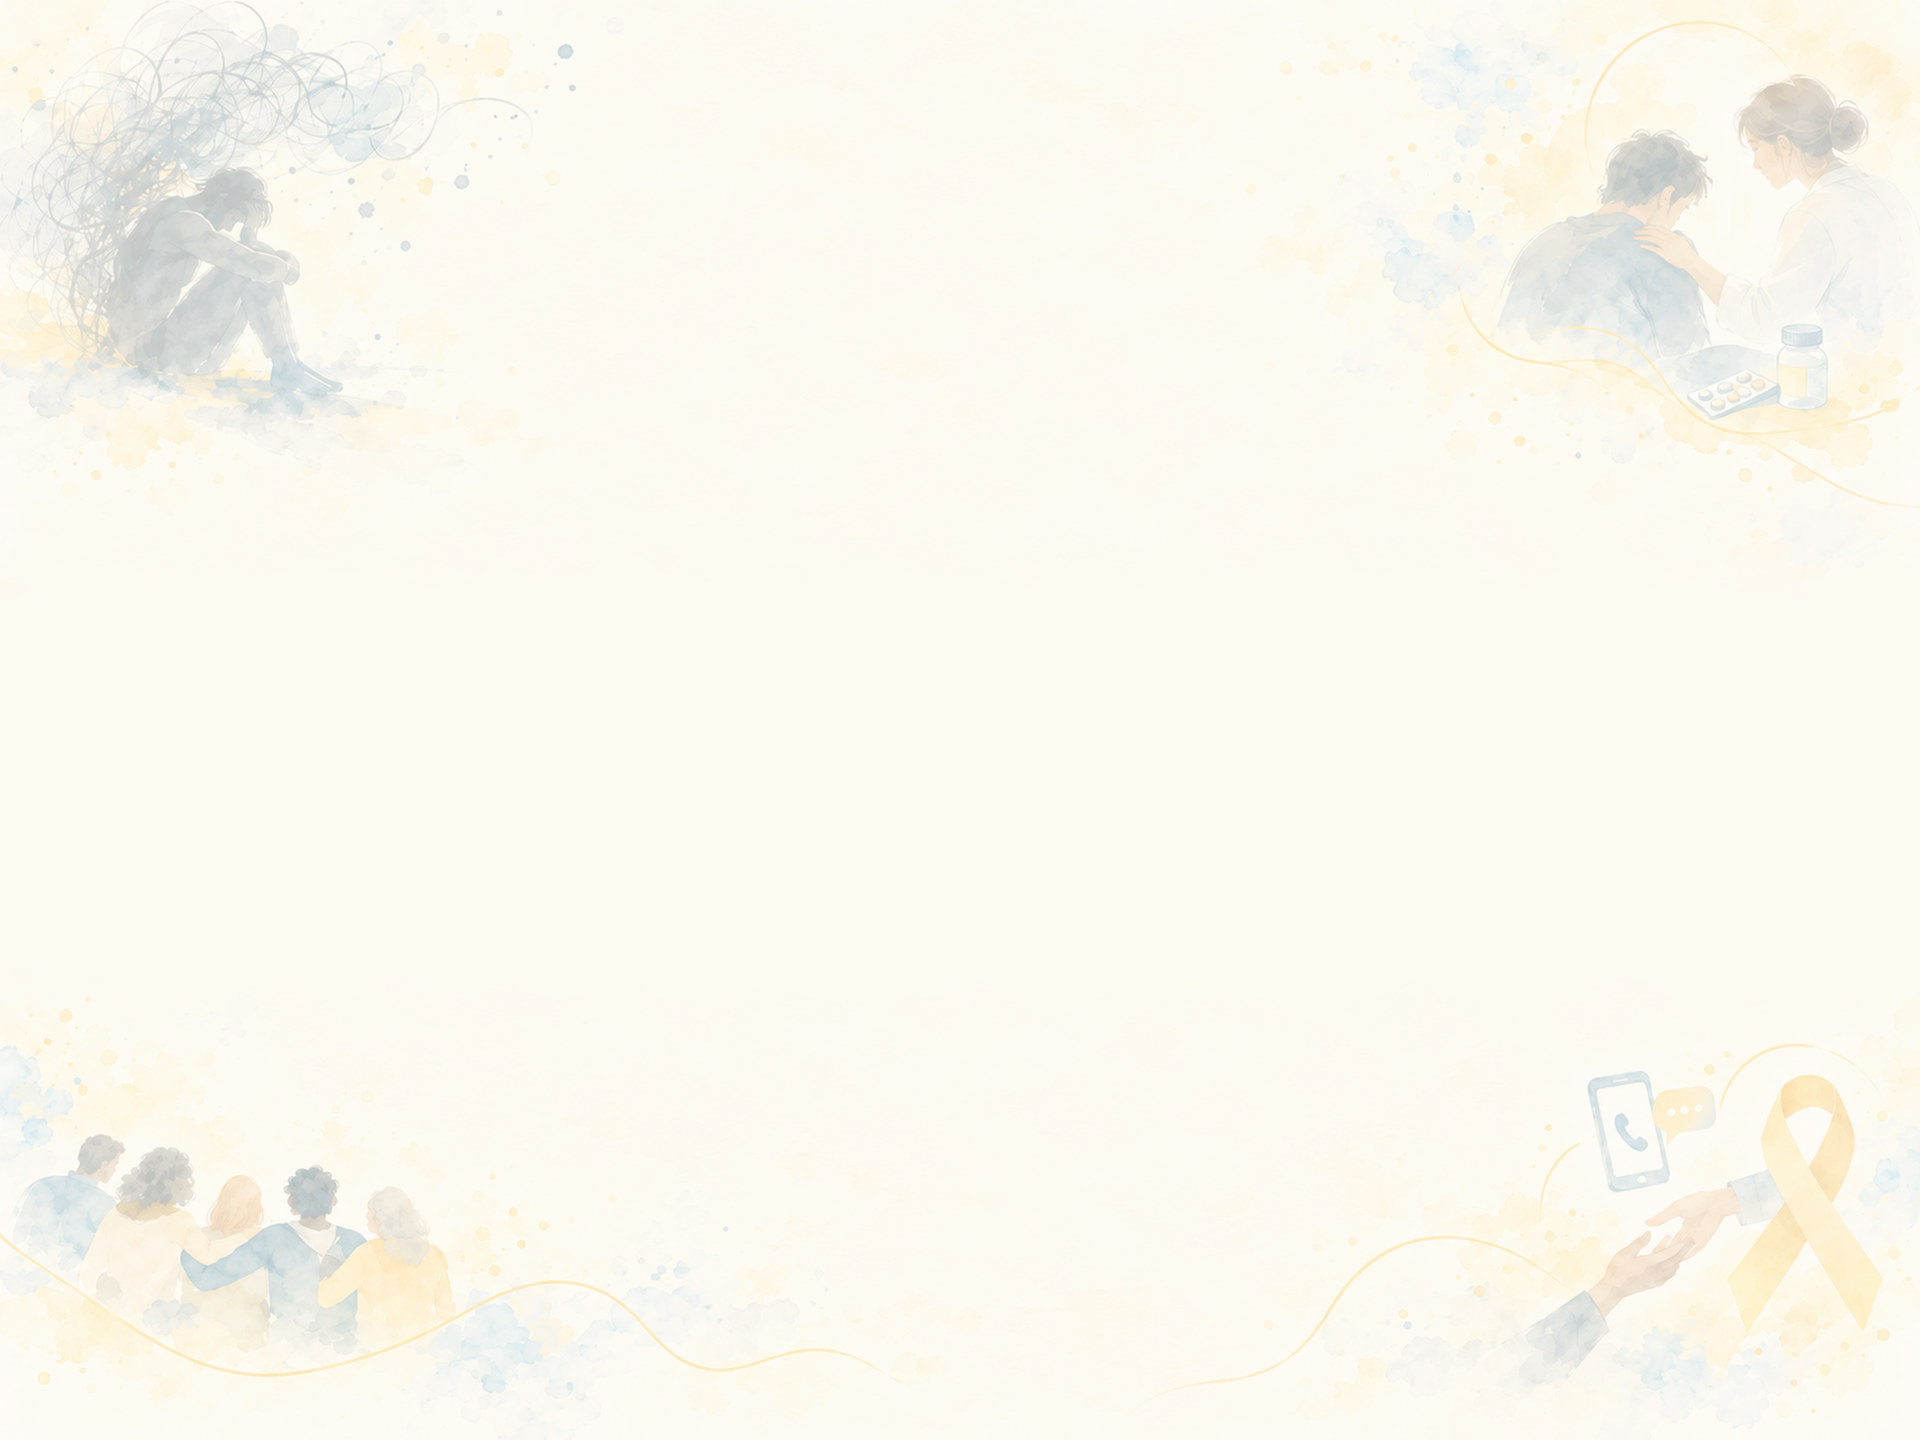
\includegraphics[width=\paperwidth,height=\paperheight]{ilustracoes/BACKGROUND.jpg}}%
  }{}
\fi

% --- Identificacao da apresentacao -------------------------------------------
\title[Risco de suic\'idio]{Risco de suic\'idio}
\subtitle{Avalia\c{c}\~ao e conduta}
\author[Prof. J. F. Musial]{Prof. Jo\~ao Frederico Musial}
\institute[Medicina | Campo Real]{Medicina | Campo Real}
\date[E3M40]{M\'odulo E3M40 \textbar{} 2026}


\begin{document}

% =============================================================================
% =============================================================================
% 00-abertura.tex - PARTE 0, abertura. Frames 01 a 03.
% =============================================================================

% ----------------------------------------------------------------- frame 01 --
% Capa. Unica excecao declarada de composicao: a ilustracao sangra de borda a
% borda e o texto ocupa a faixa central, que na arte e papel limpo. Os quatro
% cantos trazem, em sentido horario a partir do alto e a esquerda, o sofrimento
% isolado, o cuidado clinico, a rede que acolhe e o contato que se oferece, que
% e a propria cadeia da aula.
\begin{frame}[plain]
\CRar{0}
\begin{tikzpicture}[remember picture, overlay]
  \node[anchor=center, inner sep=0] at (current page.center) {%
    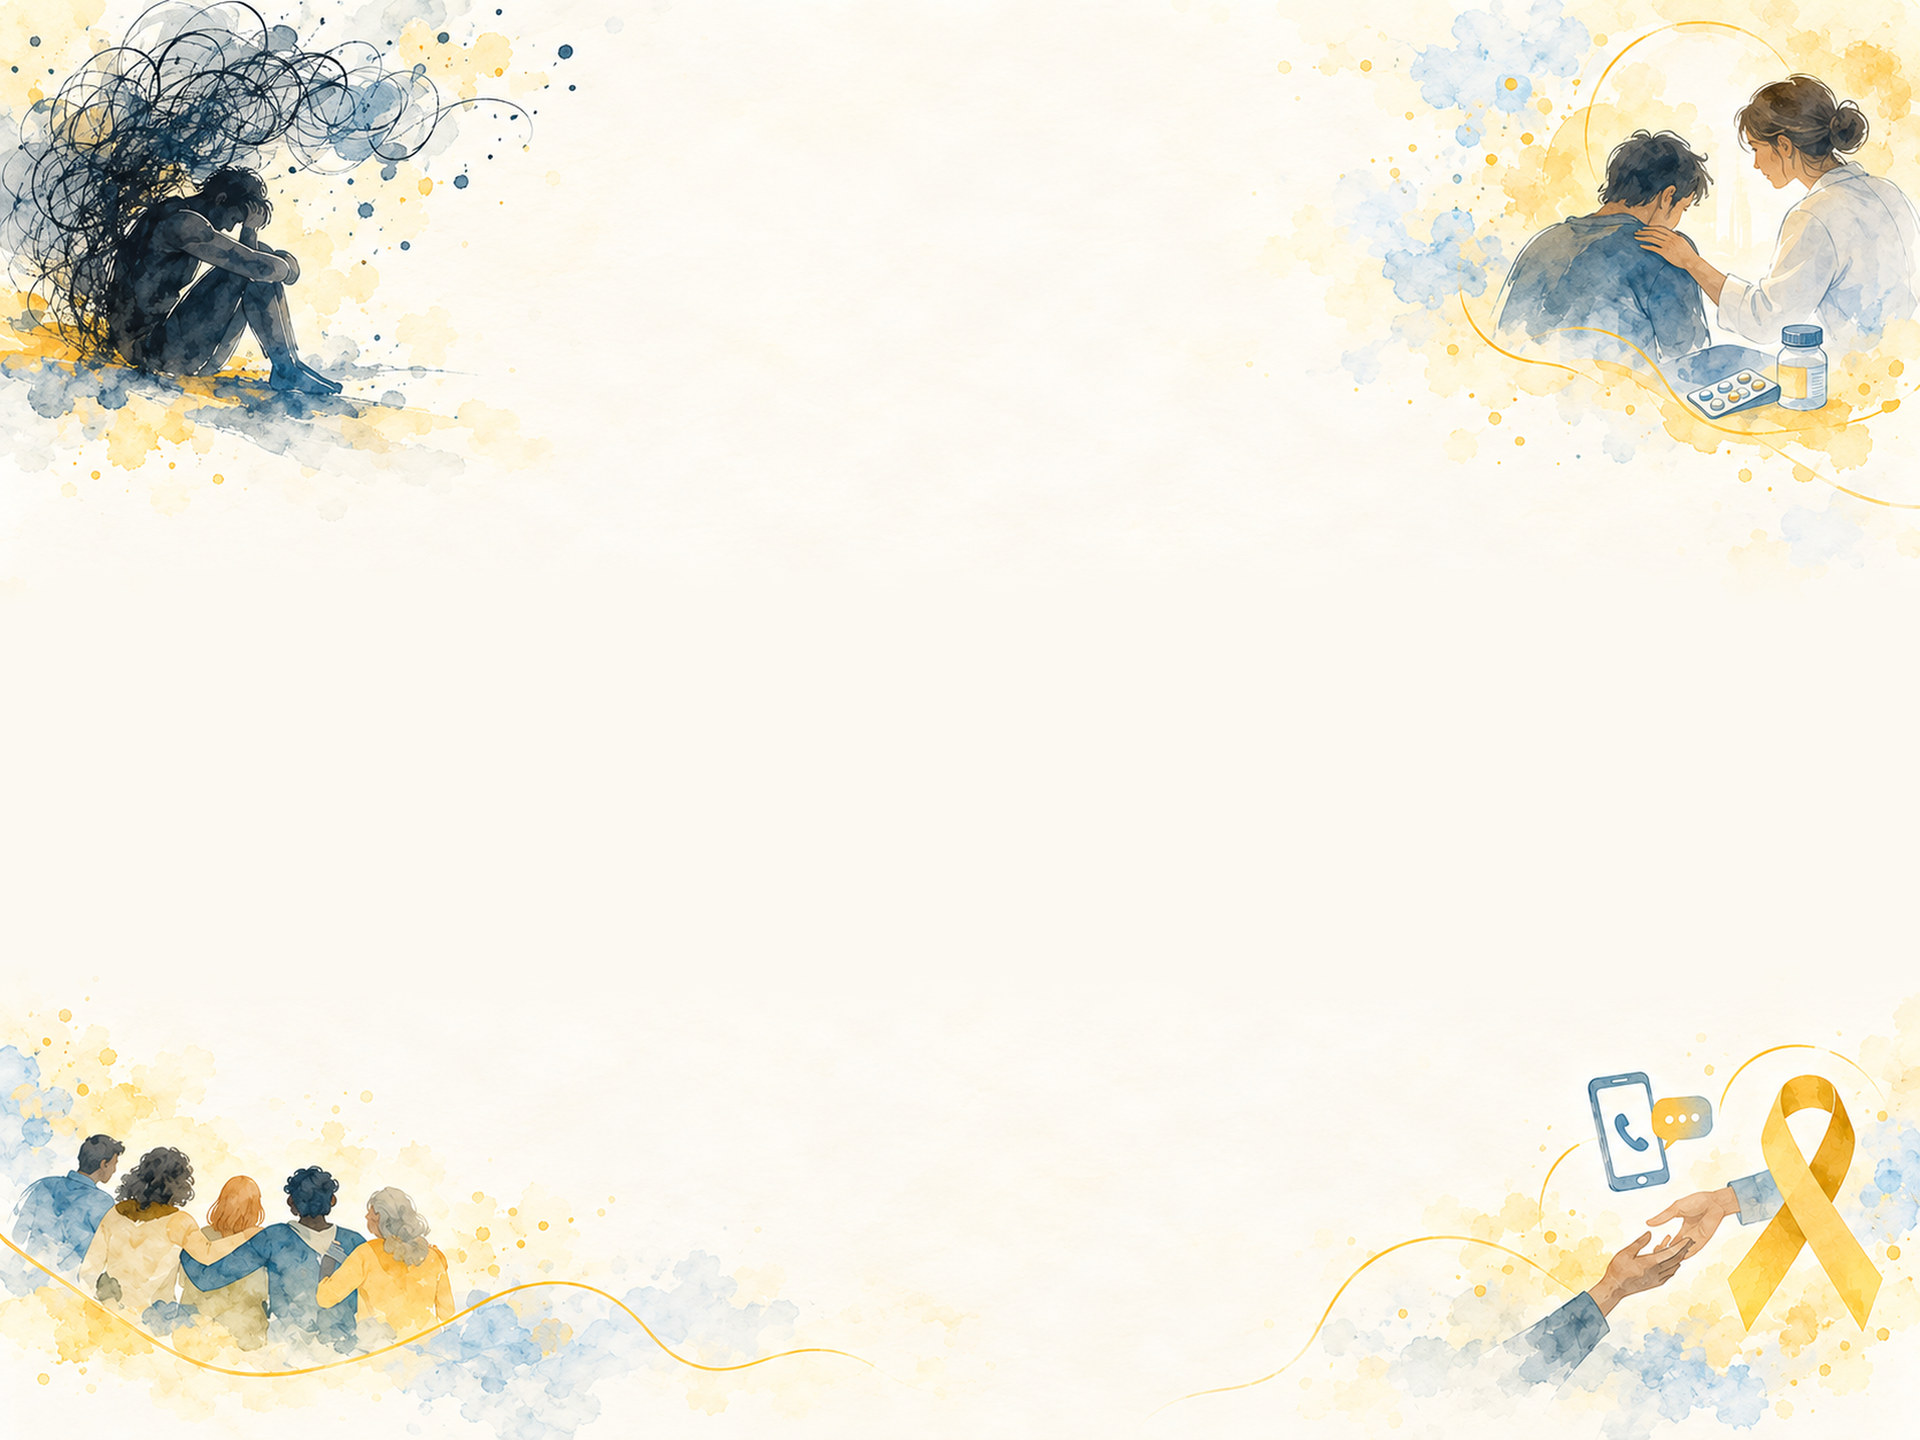
\includegraphics[width=\paperwidth, height=\paperheight]{ilustracoes/CAPA.jpg}};

  \node[anchor=center, align=center] at ($(current page.center)+(0,0.55cm)$) {%
    \begin{minipage}{8.2cm}\centering
      {\sffamily\bfseries\scriptsize\color{campobordo}%
       ATIVIDADE TE\'ORICO-PR\'ATICA}\\[0.30cm]
      {\sffamily\bfseries\LARGE\color{campoazul}Risco de suic\'idio}\\[0.14cm]
      {\sffamily\large\color{campoazul!75!black}avalia\c{c}\~ao e conduta}\\[0.34cm]
      {\color{campoamarelo!85!black}\rule{4.6cm}{1.6pt}}\\[0.30cm]
      {\sffamily\small\color{campografite}M\'odulo E3M40\\[0.05cm]
       Funcionalidade III, Cogni\c{c}\~ao e Humor}
    \end{minipage}};

  \node[anchor=south, align=center] at ($(current page.south)+(0,1.02cm)$) {%
    \begin{minipage}{7.0cm}\centering
      {\sffamily\footnotesize\color{campoazul!85!black}%
       \textbf{Prof. Jo\~ao Frederico Musial}}\\[0.06cm]
      {\sffamily\footnotesize\color{campografite}%
       Medicina \textbar{} Campo Real \textbar{} 2026}
    \end{minipage}};
\end{tikzpicture}
\end{frame}

% ----------------------------------------------------------------- frame 02 --
% Aviso de conteudo. Sobrio, sem dramatizacao, com saida garantida.
\begin{frame}{\ftit{\faHandHoldingHeart}{Antes de come\c{c}armos}}
\CRar{6}
\begin{caixaavaliar}{O que vamos discutir}
Esta aula trata de suic\'idio de forma direta, com falas de pacientes e com
decis\~oes cl\'inicas reais. N\~ao haver\'a imagem de m\'etodo, de cena nem de
les\~ao.
\end{caixaavaliar}

\CRvg
\begin{caixaproteger}{Voc\^e pode sair}
Se em algum momento voc\^e precisar se afastar, saia da sala. N\~ao \'e preciso
justificar, e isso n\~ao ser\'a registrado de nenhuma forma. Voltar depois
tamb\'em est\'a certo.
\end{caixaproteger}

\CRvg
\begin{center}
\begin{tikzpicture}
  \node[musialGreen, text width=9.2cm, font=\small] {%
    \faPhoneVolume~~\textbf{CVV 188}, liga\c{c}\~ao gratuita, 24 horas\\[2pt]
    \footnotesize O apoio ao estudante do Campo Real est\'a dispon\'ivel depois
    da aula. O docente tamb\'em est\'a.};
\end{tikzpicture}
\end{center}
\end{frame}

% ----------------------------------------------------------------- frame 03 --
% A pergunta da aula e a tese em duas linhas.
\begin{frame}{\ftit{\faQuestion}{A pergunta desta aula}}
\CRar{2.5}
\begin{center}
\begin{tikzpicture}
  \node[musialBlue, text width=9.0cm, font=\small, inner ysep=7pt] (p) {%
    \sffamily\bfseries \'E poss\'ivel construir seguran\c{c}a suficiente fora de
    um ambiente protegido neste momento?};
\end{tikzpicture}
\end{center}

\CRvg
\begin{caixaavaliar}{A tese}
O risco suicida \'e \avaliar{formula\c{c}\~ao cl\'inica din\^amica}, constru\'ida
pela intera\c{c}\~ao entre vulnerabilidades basais e modificadores proximais, e
n\~ao se reduz a escore nem a categoria. A conduta deve produzir
\proteger{seguran\c{c}a agora} e \proteger{continuidade depois}.
\end{caixaavaliar}

\CRvg
\begin{center}
\begin{tikzpicture}[node distance=0.20cm]
  \node[crnode={campoazul}{1.42cm}, font=\scriptsize, inner xsep=4pt] (a) {avaliar};
  \node[crnode={campoazul}{1.42cm}, font=\scriptsize, inner xsep=4pt, right=of a] (b) {formular};
  \node[crnode={campobordo}{1.42cm}, font=\scriptsize, inner xsep=4pt, right=of b] (c) {decidir};
  \node[crnode={campoverde}{1.70cm}, font=\scriptsize, inner xsep=4pt, right=of c] (d) {construir\\seguran\c{c}a};
  \node[crnode={campoverde}{1.70cm}, font=\scriptsize, inner xsep=4pt, right=of d] (e) {garantir\\continuidade};
  \draw[crseta=campoazul]  (a.east) -- (b.west);
  \draw[crseta=campoazul]  (b.east) -- (c.west);
  \draw[crseta=campobordo] (c.east) -- (d.west);
  \draw[crseta=campoverde] (d.east) -- (e.west);
\end{tikzpicture}
\end{center}

\mensagem{Ao final: o que, neste paciente, muda o que voc\^e far\'a nos
pr\'oximos 30 minutos?}
\end{frame}
        % frames 01 a 03
% =============================================================================
\section{O que estamos tentando entender}
% =============================================================================
% 01-fenomenologia.tex - PARTE 1, o que estamos tentando entender.
% Frames 04 a 08.
% =============================================================================

% ----------------------------------------------------------------- frame 04 --
% Primeiro frame de conteudo. Declara o recorte em uma linha e traz o mapa
% fenomenologico NAO linear, com relacoes bidirecionais.
\begin{frame}{\ftit{\faSitemap}{O que estamos tentando entender}}
\CRar{2.5}
{\footnotesize\sffamily\color{campografite}%
A prele\c{c}\~ao paralela do m\'odulo cobre o diagn\'ostico do epis\'odio
depressivo; esta ATP cobre a conduta e trata a suicidalidade como fen\^omeno
transdiagn\'ostico.\par}

\CRvg
\begin{center}
\begin{tikzpicture}[node distance=0.42cm and 0.60cm]
  \node[crnode={campoazul}{2.30cm}, font=\scriptsize]                 (pass) {idea\c{c}\~ao\\passiva};
  \node[crnode={campoazul}{2.30cm}, font=\scriptsize, right=of pass]  (ativ) {idea\c{c}\~ao\\ativa};
  \node[crnode={campoazul}{2.30cm}, font=\scriptsize, right=of ativ]  (inte) {inten\c{c}\~ao};
  \node[crnode={campoambar}{2.30cm}, font=\scriptsize, below=0.72cm of pass] (plan) {planejamento};
  \node[crnode={campoambar}{2.30cm}, font=\scriptsize, right=of plan] (prep) {comportamento\\preparat\'orio};
  \node[crnode={campobordo}{2.30cm}, font=\scriptsize, right=of prep] (tent) {tentativa};

  \draw[musialBi] (pass.east) -- (ativ.west);
  \draw[musialBi] (ativ.east) -- (inte.west);
  \draw[musialBi] (plan.east) -- (prep.west);
  \draw[musialBi] (prep.east) -- (tent.west);
  \draw[musialBi] (inte.south) -- (prep.north);
  \draw[musialBi] (ativ.south) -- (plan.north);
  \draw[musialBi, campobordo!80!black] (tent.north) to[out=60,in=0,looseness=1.5] (inte.east);
  \draw[musialBi] (plan.west) to[out=180,in=180,looseness=1.3] (pass.west);

  \node[crnode={campografite}{3.05cm}, font=\scriptsize, below=0.62cm of prep]
    (auto) {autoles\~ao sem inten\c{c}\~ao suicida\\[1pt]\scriptsize eixo paralelo};
  \draw[musialThin, dash pattern=on 2.4pt off 2pt] (auto.north) -- (prep.south);
\end{tikzpicture}
\end{center}

\mensagem{Esses fen\^omenos se relacionam nos dois sentidos. N\~ao s\~ao uma
escada obrigat\'oria.}
\end{frame}

% ----------------------------------------------------------------- frame 05 --
% A pirâmide de progressao como objeto de critica, e o eixo paralelo da autolesao.
\begin{frame}{\ftit{\faBan}{Duas leituras que atrapalham}}
\CRar{6}
\begin{columns}[onlytextwidth, t]
\begin{column}{0.47\textwidth}
\begin{caixaagir}{A escada que n\~ao existe}
Ningu\'em precisa passar por todos os degraus, na ordem, para chegar \`a
tentativa. Uma parte das tentativas ocorre em quem nunca planejou, e uma parte
de quem planeja durante anos nunca tenta.\par
\agir{Consequ\^encia:} a aus\^encia de um degrau anterior n\~ao tranquiliza.
\end{caixaagir}
\end{column}
\calha
\begin{column}{0.47\textwidth}
\begin{caixaavaliar}{A autoles\~ao no eixo ao lado}
A autoles\~ao sem inten\c{c}\~ao suicida tem fun\c{c}\~ao de regula\c{c}\~ao do
sofrimento, e n\~ao de morte. N\~ao \'e tentativa.\par
\avaliar{E ainda assim} \'e um dos marcadores mais consistentes de risco
futuro. As duas coisas s\~ao verdadeiras ao mesmo tempo.
\end{caixaavaliar}
\end{column}
\end{columns}

\CRvg
\begin{center}
\begin{tikzpicture}
  \node[crnode={campografite}{9.6cm}, font=\scriptsize] {%
    Dizer \fala{ele s\'o tem idea\c{c}\~ao passiva} e encerrar a\'i \'e usar um
    degrau como se fosse um progn\'ostico.};
\end{tikzpicture}
\end{center}
\end{frame}

% ----------------------------------------------------------------- frame 06 --
% Magnitude e tendencia. pgfplots. Apenas os dois pontos documentados.
\begin{frame}{\ftit{\faChartLine}{Magnitude e tend\^encia no Brasil}}
\CRar{4.6}
\begin{columns}[onlytextwidth, T]
\begin{column}{0.50\textwidth}
\begin{center}
\begin{tikzpicture}
\begin{axis}[
  width=5.4cm, height=4.2cm,
  ymin=0, ymax=9, xmin=2008.6, xmax=2022.4,
  xtick={2010,2021}, xticklabels={2010,2021},
  ytick={0,2,4,6,8},
  ylabel={\scriptsize \'obitos por 100 mil},
  y label style={font=\scriptsize, color=campografite},
  tick label style={font=\scriptsize, color=campografite},
  axis line style={campografite!55},
  grid=major, grid style={campografite!14, line width=0.3pt},
  every axis plot/.append style={line width=1.1pt}]
  \addplot[campoazul!85!black, mark=*, mark size=2.3pt,
           mark options={fill=campoazul!25, draw=campoazul!85!black}]
    coordinates {(2010,5.2) (2021,7.5)};
  \node[font=\scriptsize\sffamily, color=campoazul!85!black, anchor=south east]
    at (axis cs:2010,5.2) {5,2};
  \node[font=\scriptsize\sffamily, color=campoazul!85!black, anchor=south east]
    at (axis cs:2021,7.5) {7,5};
\end{axis}
\end{tikzpicture}
\end{center}
{\scriptsize\sffamily\color{campografite}\hspace{0.3cm}Dois pontos documentados.
A s\'erie intermedi\'aria n\~ao foi reconstru\'ida.\par}
\end{column}
\calha
\begin{column}{0.44\textwidth}
\begin{caixaavaliar}{2021, no Brasil}
\begin{itemc}
\item \avaliar{15.507} mortes por suic\'idio
\item \avaliar{114.159} notifica\c{c}\~oes de les\~ao autoprovocada
\item taxa de \avaliar{7,5} por 100 mil, \mudanca{42\% acima} da taxa de 2010
\end{itemc}
\end{caixaavaliar}
\CRvg
\begin{caixamudanca}{O que essa raz\~ao diz}
Para cada morte registrada h\'a cerca de sete notifica\c{c}\~oes de les\~ao
autoprovocada. Essas pessoas passam pelo servi\c{c}o.
\end{caixamudanca}
\end{column}
\end{columns}
\fonte{Minist\'erio da Sa\'ude, Boletim Epidemiol\'ogico v.\,55, n.\,4, 2024,
com dados do SIM e do SINAN.}
\end{frame}

% ----------------------------------------------------------------- frame 07 --
% Faixas etarias e sexo. Barras agrupadas, dado numericamente publicado.
\begin{frame}{\ftit{\faUsers}{Quem morre, por faixa et\'aria e sexo}}
\CRar{6}
\begin{center}
\begin{tikzpicture}
\begin{axis}[
  width=10.6cm, height=5.0cm,
  ybar=1.4pt, bar width=8.5pt,
  ymin=0, ymax=23, ytick={0,5,10,15,20},
  symbolic x coords={5 a 14,15 a 19,20 a 29,30 a 49,50 a 69,70 ou mais},
  xtick=data,
  ylabel={\scriptsize \'obitos por 100 mil, 2021},
  y label style={font=\scriptsize, color=campografite},
  tick label style={font=\scriptsize, color=campografite},
  axis line style={campografite!55},
  ymajorgrids, grid style={campografite!14, line width=0.3pt},
  legend style={font=\scriptsize\sffamily, draw=campografite!35, at={(0.015,0.98)},
                anchor=north west, legend columns=2, column sep=5pt},
  nodes near coords, nodes near coords style={font=\tiny\sffamily,
                                             color=campografite},
  every node near coord/.append style={/pgf/number format/.cd, fixed,
                                       precision=1, use comma}]
  \addplot[draw=campoazul!85!black, fill=campoazul!30,
           every node near coord/.append style={/tikz/.cd, yshift=5.5pt, xshift=-2.6pt}]
    coordinates {(5 a 14,0.7) (15 a 19,9.3) (20 a 29,14.6) (30 a 49,14.9)
                 (50 a 69,15.4) (70 ou mais,18.1)};
  \addplot[draw=camporoxo!80!black, fill=camporoxo!22,
           every node near coord/.append style={/tikz/.cd, xshift=2.6pt}]
    coordinates {(5 a 14,0.9) (15 a 19,4.5) (20 a 29,3.9) (30 a 49,3.8)
                 (50 a 69,3.8) (70 ou mais,2.9)};
  \legend{homens, mulheres}
\end{axis}
\end{tikzpicture}
\end{center}

\mensagem{A taxa mais alta est\'a nos homens com 70 anos ou mais. \'E a faixa que
o servi\c{c}o menos pergunta.}
\fonte{Minist\'erio da Sa\'ude, Boletim Epidemiol\'ogico v.\,55, n.\,4, 2024.}
\end{frame}

% ----------------------------------------------------------------- frame 08 --
% Contato previo com servicos. O argumento que sustenta toda a aula.
\begin{frame}{\ftit{\faUserMd}{Eles passam por n\'os antes}}
\CRar{6}
\begin{center}
\begin{tikzpicture}
\begin{axis}[
  width=9.55cm, height=4.10cm,
  xbar, bar width=11pt,
  xmin=0, xmax=100,
  symbolic y coords={smm, apm, sma, apa},
  ytick=data,
  yticklabels={{sa\'ude mental, no m\^es},
               {aten\c{c}\~ao prim\'aria, no m\^es},
               {sa\'ude mental, no ano},
               {aten\c{c}\~ao prim\'aria, no ano}},
  yticklabel style={font=\scriptsize, color=campografite, align=right},
  xlabel={\scriptsize \% das pessoas que morreram por suic\'idio},
  x label style={font=\scriptsize, color=campografite},
  tick label style={font=\scriptsize, color=campografite},
  axis line style={campografite!55},
  enlarge y limits=0.20,
  xmajorgrids, grid style={campografite!14, line width=0.3pt},
  nodes near coords, nodes near coords style={font=\tiny\sffamily,
                                              color=campografite, anchor=west,
                                              xshift=1.5pt},
  point meta=explicit symbolic]
  \addplot[draw=campoazul!85!black, fill=campoazul!30]
    coordinates {(20,smm)[20\%] (45,apm)[45\%]
                 (33,sma)[33\%] (75,apa)[75\%]};
\end{axis}
\end{tikzpicture}
\end{center}

\begin{caixaavaliar}{O que isso obriga}
A pessoa que morre por suic\'idio costuma ter estado diante de um m\'edico pouco
antes, e quase sempre de um m\'edico que n\~ao era psiquiatra. Em idosos, o
contato com a aten\c{c}\~ao prim\'aria no m\^es anterior \'e ainda mais
frequente do que em adultos jovens.
\end{caixaavaliar}

\fonte{Luoma, Martin e Pearson, \emph{Am J Psychiatry} 2002, revis\~ao de 40
estudos. \seloevidencia}
\end{frame}
   % frames 04 a 08
% =============================================================================
\section{Como perguntar}
% =============================================================================
% 02-entrevista.tex - PARTE 2, como perguntar. Frames 09 a 15.
% Frases LITERAIS na tela, nao parafrases.
% =============================================================================

% ----------------------------------------------------------------- frame 09 --
\begin{frame}{\ftit{\faCommentDots}{Perguntar n\~ao cria suicidalidade}}
\CRar{2.4}
\begin{caixaavaliar}{O receio e a evid\^encia}
O receio de que perguntar sobre suic\'idio possa induzir a ideia \'e comum e
n\~ao se sustenta. Revis\~ao da literatura publicada n\~ao encontrou, em
nenhum dos estudos revisados, aumento estatisticamente significativo de
idea\c{c}\~ao suicida entre os participantes que foram perguntados.
\end{caixaavaliar}

\CRvg
\begin{columns}[onlytextwidth, t]
\begin{column}{0.47\textwidth}
\begin{caixaproteger}{O que perguntar produz}
\begin{itemc}
\item nomeia o que o paciente n\~ao sabia como dizer
\item mostra que o assunto cabe nesta consulta
\item permite a pergunta seguinte
\end{itemc}
\end{caixaproteger}
\end{column}
\calha
\begin{column}{0.47\textwidth}
\begin{caixaagir}{O que n\~ao perguntar produz}
\begin{itemc}
\item um registro que diz apenas \fala{nega idea\c{c}\~ao}
\item uma alta que ningu\'em consegue justificar depois
\item a impress\~ao, no paciente, de que aquilo n\~ao se fala aqui
\end{itemc}
\end{caixaagir}
\end{column}
\end{columns}

\fonte{Dazzi, Gribble, Wessely e Fear, \emph{Psychol Med} 2014, revis\~ao em
formato de editorial. \seloevidencia}
\end{frame}

% ----------------------------------------------------------------- frame 10 --
\begin{frame}{\ftit{\faEye}{Reconhecer a pista}}
\CRar{2.6}
{\small Estas falas chegam ao pronto atendimento por outro motivo. Elas s\~ao a
abertura, e n\~ao a queixa.\par}

\CRvg
\begin{columns}[onlytextwidth, t]
\begin{column}{0.47\textwidth}
\begin{caixaavaliar}{O que o paciente diz}
\begin{itemc}
\item \fala{eu queria dormir e n\~ao acordar}
\item \fala{assim n\~ao d\'a mais}
\item \fala{eles ficariam melhor sem mim}
\item \fala{eu estou s\'o cansado, doutor}
\item \fala{n\~ao sei quanto tempo eu aguento}
\end{itemc}
\end{caixaavaliar}
\end{column}
\calha
\begin{column}{0.47\textwidth}
\begin{caixamudanca}{O que a fam\'ilia diz}
\begin{itemc}
\item \fala{ele deu as coisas dele}
\item \fala{ela ficou estranhamente calma}
\item \fala{ele se despediu de um jeito esquisito}
\item \fala{ela parou de atender o telefone}
\item \fala{ele acertou tudo o que estava pendente}
\end{itemc}
\end{caixamudanca}
\end{column}
\end{columns}

\mensagem{Toda pista reconhecida obriga \`a pergunta seguinte. Reconhecer e n\~ao
perguntar \'e pior do que n\~ao ter reconhecido.}
\end{frame}

% ----------------------------------------------------------------- frame 11 --
\begin{frame}{\ftit{\faComments}{A frase de transi\c{c}\~ao}}
\CRar{4.3}
{\footnotesize Esta \'e a frase. N\~ao \'e exemplo do que dizer, \'e o que se
diz.\par}

\CRvg
\begin{center}
\begin{tikzpicture}
  \node[musialBlue, text width=9.4cm, font=\footnotesize, inner ysep=6pt] {%
    \itshape\guillemotleft Pelo que voc\^e est\'a me contando, esse sofrimento
    est\'a bem pesado. Quando as pessoas chegam assim, \`as vezes pensam em
    morrer. Voc\^e tem tido esses pensamentos?\guillemotright};
\end{tikzpicture}
\end{center}

\CRvg
\begin{columns}[onlytextwidth, t]
\begin{column}{0.47\textwidth}
\begin{caixaproteger}{Por que funciona}
Nomeia o sofrimento antes de perguntar, universaliza sem banalizar, e faz uma
pergunta fechada que o paciente consegue responder com uma palavra.
\end{caixaproteger}
\end{column}
\calha
\begin{column}{0.47\textwidth}
\begin{caixaagir}{O que n\~ao dizer}
\fala{Voc\^e n\~ao est\'a pensando em fazer besteira, est\'a?}\par
\vspace{0.06cm}
A pergunta j\'a traz a resposta esperada.
\end{caixaagir}
\end{column}
\end{columns}
\end{frame}

% ----------------------------------------------------------------- frame 12 --
% Roteiro de perguntas. Uma das tres tabelas autorizadas na aula.
\begin{frame}{\ftit{\faSearch}{Caracterizar a idea\c{c}\~ao}}
\CRar{2.2}
\begin{CRtabela}
\begin{center}
\begin{tabular}{E P{4.05cm} P{4.05cm}}
\toprule
\rowcolor{campoazul!10}
\textbf{O que caracterizar} & \textbf{Como perguntar} & \textbf{O que muda} \\
\midrule
existe & \fala{voc\^e tem tido esses pensamentos?} & abre ou fecha toda a
sequ\^encia \\
frequ\^encia & \fala{quantas vezes, num dia como o de ontem?} & separa o
epis\'odico do cont\'inuo \\
dura\c{c}\~ao & \fala{quando vem, fica quanto tempo?} & minutos e horas pedem
condutas diferentes \\
intrusividade & \fala{ele vem sozinho ou voc\^e o chama?} & pensamento que
invade cansa e desgasta \\
capacidade de afastar & \fala{quando vem, voc\^e consegue empurrar? o que
ajuda?} & \'e aqui que mora o plano de seguran\c{c}a \\
\bottomrule
\end{tabular}
\end{center}
\end{CRtabela}

\mensagem{A \'ultima linha \'e a mais \'util das cinco, e \'e a que quase
ningu\'em pergunta.}
\end{frame}

% ----------------------------------------------------------------- frame 13 --
\begin{frame}{\ftit{\faRoute}{Inten\c{c}\~ao, plano e prepara\c{c}\~ao}}
\CRar{6}
\begin{center}
\begin{tikzpicture}[node distance=0.34cm]
  \node[crnode={campoazul}{2.55cm}, font=\scriptsize] (i) {\textbf{inten\c{c}\~ao}\\[1pt]
    \fala{voc\^e quer morrer ou quer que isso pare?}};
  \node[crnode={campoambar}{2.55cm}, font=\scriptsize, right=of i] (p) {\textbf{plano}\\[1pt]
    \fala{voc\^e chegou a pensar em como faria?}};
  \node[crnode={campoambar}{2.55cm}, font=\scriptsize, right=of p] (r) {\textbf{prepara\c{c}\~ao}\\[1pt]
    \fala{voc\^e chegou a fazer alguma coisa nessa dire\c{c}\~ao?}};
  \draw[crseta=campoazul] (i.east) -- (p.west);
  \draw[crseta=campoambar] (p.east) -- (r.west);
\end{tikzpicture}
\end{center}

\CRvg
\begin{columns}[onlytextwidth, t]
\begin{column}{0.47\textwidth}
\begin{caixaavaliar}{A pergunta que falta}
Depois de \fala{fez alguma coisa?}, vem \fala{mesmo que depois voc\^e tenha
desistido}. \'E essa segunda metade que autoriza o paciente a contar o ato
interrompido.
\end{caixaavaliar}
\end{column}
\calha
\begin{column}{0.47\textwidth}
\begin{caixaagir}{O que n\~ao entra na tela nem na pergunta}
N\~ao se pergunta detalhe de m\'etodo por curiosidade cl\'inica, e n\~ao se
compara letalidade diante do paciente. O que importa \'e a exist\^encia do
acesso e a possibilidade de restringi-lo.
\end{caixaagir}
\end{column}
\end{columns}
\end{frame}

% ----------------------------------------------------------------- frame 14 --
\begin{frame}{\ftit{\faClock}{Comportamento e temporalidade}}
\CRar{1.3}
\begin{caixamudanca}{A pergunta que organiza o tempo}
\fala{O que mudou nas \'ultimas horas? E nos \'ultimos dias?}
\end{caixamudanca}

\CRvg
\begin{center}
\begin{tikzpicture}[node distance=0.30cm]
  \node[crnode={campografite}{2.15cm}, font=\scriptsize] (v) {meses e anos\\[1pt]
    \scriptsize vulnerabilidade};
  \node[crnode={campoambar}{2.15cm}, font=\scriptsize, right=of v] (s) {\'ultimas semanas\\[1pt]
    \scriptsize deteriora\c{c}\~ao};
  \node[crnode={campoambar}{2.15cm}, font=\scriptsize, right=of s] (d) {\'ultimos dias\\[1pt]
    \scriptsize prepara\c{c}\~ao};
  \node[crnode={campobordo}{2.15cm}, font=\scriptsize, right=of d] (h) {\'ultimas horas\\[1pt]
    \scriptsize decis\~ao de hoje};
  \draw[musialThin] (v.east) -- (s.west);
  \draw[crseta=campoambar] (s.east) -- (d.west);
  \draw[crseta=campobordo] (d.east) -- (h.west);
\end{tikzpicture}
\end{center}

\CRvg
\begin{columns}[onlytextwidth, t]
\begin{column}{0.47\textwidth}
\begin{caixaavaliar}{O que perguntar do comportamento}
\begin{itemc}
\item o que fez, n\~ao s\'o o que pensou
\item o que interrompeu o ato, quando houve
\item o que estava acontecendo naquela hora
\end{itemc}
\end{caixaavaliar}
\end{column}
\calha
\begin{column}{0.47\textwidth}
\begin{caixamudanca}{Mudan\c{c}as que pesam}
\begin{itemc}
\item sono que encurtou de repente
\item retraimento que apertou nos \'ultimos dias
\item algo resolvido ou acertado sem explica\c{c}\~ao
\end{itemc}
\end{caixamudanca}
\end{column}
\end{columns}
\end{frame}

% ----------------------------------------------------------------- frame 15 --
\begin{frame}{\ftit{\faBolt}{O que modifica a seguran\c{c}a agora}}
\CRar{6}
\begin{center}
\begin{tikzpicture}[node distance=0.26cm and 0.30cm]
  \node[musialCenter, minimum size=1.95cm, font=\scriptsize\bfseries\sffamily] (c)
    {modificadores\\proximais};

  \node[crnode={campoambar}{1.85cm}, font=\scriptsize, above left=0.60cm and 0.75cm of c] (subs) {subst\^ancias};
  \node[crnode={campoambar}{1.85cm}, font=\scriptsize, above=0.60cm of c] (agit) {agita\c{c}\~ao};
  \node[crnode={campoambar}{1.85cm}, font=\scriptsize, above right=0.60cm and 0.75cm of c] (ins) {ins\^onia};
  \node[crnode={campobordo}{1.85cm}, font=\scriptsize, left=0.80cm of c] (psic) {psicose};
  \node[crnode={campobordo}{1.85cm}, font=\scriptsize, right=0.80cm of c] (imp) {impulsividade};
  \node[crnode={campoazul}{1.85cm}, font=\scriptsize, below left=0.60cm and 0.75cm of c] (perd) {perdas recentes};
  \node[crnode={campoverde}{1.85cm}, font=\scriptsize, below=0.60cm of c] (rede) {rede dispon\'ivel};
  \node[crnode={campoverde}{1.85cm}, font=\scriptsize, below right=0.60cm and 0.75cm of c] (colab) {capacidade de colaborar};

  \draw[musialThin] (subs.south east) -- (c.north west);
  \draw[musialThin] (agit.south) -- (c.north);
  \draw[musialThin] (ins.south west) -- (c.north east);
  \draw[musialThin] (psic.east) -- (c.west);
  \draw[musialThin] (imp.west) -- (c.east);
  \draw[musialThin] (perd.north east) -- (c.south west);
  \draw[musialThin] (rede.north) -- (c.south);
  \draw[musialThin] (colab.north west) -- (c.south east);
\end{tikzpicture}
\end{center}

\mensagem{Supervis\~ao dispon\'ivel e capacidade de colaborar s\~ao
modificadores, e n\~ao detalhe de execu\c{c}\~ao do plano.}
\end{frame}
      % frames 09 a 15
% =============================================================================
\section{Como formular}
% =============================================================================
% 03-formulacao.tex - PARTE 3, como formular. Frames 16 a 20.
% A matriz comum em tela unica e depois desdobrada.
% =============================================================================

% ----------------------------------------------------------------- frame 16 --
% A MATRIZ COMUM, tela unica. Todos os frames seguintes desdobram esta.
\begin{frame}{\ftit{\faClipboardList}{A matriz da formula\c{c}\~ao}}
\CRar{6}
\begin{center}
\begin{tikzpicture}
  \node[crnode={campografite}{1.95cm}, font=\scriptsize, inner xsep=4pt,
        minimum height=1.05cm] (v) at (0,0) {vulnerabilidades\\basais};
  \node[font=\footnotesize\bfseries\color{campografite},
        right=0.09cm of v] (m1) {+};
  \node[crnode={campoambar}{1.60cm}, font=\scriptsize, inner xsep=4pt,
        minimum height=1.05cm, right=0.09cm of m1] (p) {modificadores\\proximais};
  \node[font=\footnotesize\bfseries\color{campografite},
        right=0.09cm of p] (m2) {+};
  \node[crnode={campoazul}{1.60cm}, font=\scriptsize, inner xsep=4pt,
        minimum height=1.05cm, right=0.09cm of m2] (s) {suicidalidade\\atual};
  \node[font=\footnotesize\bfseries\color{campografite},
        right=0.09cm of s] (m3) {+};
  \node[crnode={campobordo}{1.60cm}, font=\scriptsize, inner xsep=4pt,
        minimum height=1.05cm, right=0.09cm of m3] (a) {acesso\\a meios};

  \node[crnode={campoverde}{4.00cm}, font=\scriptsize, inner xsep=4pt,
        minimum height=0.78cm] (c) at ($(v.south)!0.5!(p.south) + (0,-1.05)$)
    {capacidade de construir seguran\c{c}a};
  \node[crnode={campoazul}{2.95cm}, font=\small, inner xsep=4pt,
        minimum height=0.78cm] (f) at ($(s.south)!0.5!(a.south) + (0.25,-1.05)$)
    {\textbf{formula\c{c}\~ao}};

  \draw[musialThin] (v.south) |- ($(c.north)+(0,0.28)$) -- (c.north);
  \draw[musialThin] (p.south) -- ($(p.south)+(0,-0.28)$) -- (c.north);
  \draw[crseta=campoazul]  (s.south) -- ($(s.south)+(0,-0.28)$) -- (f.north);
  \draw[crseta=campobordo] (a.south) |- ($(f.north)+(0,0.28)$) -- (f.north);
  \draw[crseta=campoverde] (c.east) -- (f.west);
\end{tikzpicture}
\end{center}

\CRvg
\begin{center}
\begin{tikzpicture}
  \node[musialBlue, text width=9.3cm, font=\small, inner ysep=7pt] {%
    \sffamily\bfseries \'E poss\'ivel construir seguran\c{c}a suficiente fora de
    um ambiente protegido neste momento?};
\end{tikzpicture}
\end{center}

\mensagem{A sa\'ida da matriz \'e uma pergunta que se responde com conduta, e
n\~ao uma etiqueta.}
\end{frame}

% ----------------------------------------------------------------- frame 17 --
\begin{frame}{\ftit{\faHourglassHalf}{Vulnerabilidades basais e modificadores proximais}}
\CRar{2}
\begin{columns}[onlytextwidth, t]
\begin{column}{0.47\textwidth}
\begin{caixanorma}{Vulnerabilidades basais}
O que este paciente carrega h\'a meses ou anos.
\begin{itemc}
\item transtorno mental em curso
\item tentativa pr\'evia, o preditor isolado mais forte
\item autoles\~ao recorrente
\item doen\c{c}a dolorosa ou incapacitante
\item isolamento e perda de papel social
\end{itemc}
\end{caixanorma}
\end{column}
\calha
\begin{column}{0.47\textwidth}
\begin{caixamudanca}{Modificadores proximais}
O que est\'a diferente nesta semana e nesta noite.
\begin{itemc}
\item intoxica\c{c}\~ao, agita\c{c}\~ao, ins\^onia
\item psicose e impulsividade
\item perda, humilha\c{c}\~ao, ruptura recente
\item mudan\c{c}a de tratamento ou alta recente
\item rede que deixou de estar dispon\'ivel
\end{itemc}
\end{caixamudanca}
\end{column}
\end{columns}

\mensagem{A vulnerabilidade explica por que este paciente, e n\~ao outro. O
modificador explica por que hoje, e n\~ao no m\^es passado.}
\end{frame}

% ----------------------------------------------------------------- frame 18 --
\begin{frame}{\ftit{\faKey}{Suicidalidade atual e acesso a meios}}
\CRar{6}
\begin{columns}[onlytextwidth, t]
\begin{column}{0.47\textwidth}
\begin{caixaavaliar}{Suicidalidade atual}
O que foi caracterizado na entrevista, em vez de resumido em uma palavra:
frequ\^encia, dura\c{c}\~ao, intrusividade, capacidade de afastar,
inten\c{c}\~ao, plano e prepara\c{c}\~ao, com a data do que houve.
\end{caixaavaliar}
\end{column}
\calha
\begin{column}{0.47\textwidth}
\begin{caixaagir}{Acesso a meios}
Tr\^es perguntas, e nenhuma sobre m\'etodo:
\begin{itemc}
\item existe acesso agora?
\item \'e concretamente poss\'ivel restringir?
\item quem da rede participa dessa restri\c{c}\~ao?
\end{itemc}
\end{caixaagir}
\end{column}
\end{columns}

\CRvg
\begin{center}
\begin{tikzpicture}
  \node[crnode={campografite}{9.5cm}, font=\scriptsize] {%
    A pergunta sobre arma de fogo na resid\^encia \'e obrigat\'oria e quase nunca
    aparece no registro. A aus\^encia dela \'e a falha mais comum destes
    atendimentos.};
\end{tikzpicture}
\end{center}
\end{frame}

% ----------------------------------------------------------------- frame 19 --
\begin{frame}{\ftit{\faHandsHelping}{Capacidade de construir seguran\c{c}a}}
\CRar{3.3}
{\small \'E o elemento que os outros quatro n\~ao mostram, e o que mais muda a
conduta.\par}

\CRvg
\begin{columns}[onlytextwidth, t]
\begin{column}{0.47\textwidth}
\begin{caixaproteger}{Sustenta o plano}
\begin{itemc}
\item comunica o que sente a algu\'em
\item aceita que a rede seja acionada
\item pactua o que far\'a se piorar
\item consegue reduzir o acesso hoje
\item tem quem permane\c{c}a com ele
\end{itemc}
\end{caixaproteger}
\end{column}
\calha
\begin{column}{0.47\textwidth}
\begin{caixaagir}{N\~ao sustenta o plano}
\begin{itemc}
\item oculta a situa\c{c}\~ao da fam\'ilia
\item recusa a participa\c{c}\~ao da rede
\item n\~ao consegue pactuar nada concreto
\item n\~ao colabora por psicose ou intoxica\c{c}\~ao
\item tem rede que existe e n\~ao sustenta
\end{itemc}
\end{caixaagir}
\end{column}
\end{columns}

\mensagem{Rede dispon\'ivel n\~ao \'e o mesmo que supervis\~ao poss\'ivel.
Pergunte o que aquela pessoa consegue fazer, e at\'e quando.}
\end{frame}

% ----------------------------------------------------------------- frame 20 --
% A critica ao semaforo. O unico lugar em que baixo, moderado e alto aparecem.
\begin{frame}{\ftit{\faTimes}{O que a matriz substitui}}
\CRar{4.6}
\begin{center}
\begin{tikzpicture}[node distance=0.22cm]
  \node[crnode={campografite}{1.38cm}, font=\scriptsize, inner xsep=4pt] (b) {baixo};
  \node[crnode={campografite}{1.38cm}, font=\scriptsize, inner xsep=4pt, right=of b] (m) {moderado};
  \node[crnode={campografite}{1.38cm}, font=\scriptsize, inner xsep=4pt, right=of m] (a) {alto};
  \node[font=\large\color{campobordo}, right=0.26cm of a] (x) {\faTimes};
  \node[crnode={campoazul}{3.30cm}, font=\scriptsize, inner xsep=4pt, right=0.26cm of x] (q)
    {\'E poss\'ivel construir seguran\c{c}a fora daqui agora?};
\end{tikzpicture}
\end{center}

\CRvg
\begin{caixaagir}{Por que o sem\'aforo n\~ao resolve}
A categoria n\~ao diz o que fazer. Dois pacientes classificados como risco
moderado podem exigir condutas opostas, e a classifica\c{c}\~ao n\~ao registra
nem o que sustenta a decis\~ao nem o que precisaria mudar para invert\^e-la.
Escalas ajudam a n\~ao esquecer perguntas e n\~ao decidem conduta.
\end{caixaagir}

\CRvg
\begin{caixaproteger}{O que a pergunta operacional entrega}
Uma resposta que j\'a \'e conduta, com as duas sa\'idas explicitadas, e um
registro que permite reconstruir depois por que a decis\~ao foi aquela.
\end{caixaproteger}
\end{frame}
      % frames 16 a 20
% =============================================================================
% 03b-contextos.tex - PARTE 3B, contextos que a matriz nao resolve sozinha.
% Frames 21 e 22. Gabarito fixo: macro unica \quadroDx, geometria identica,
% dois quadros por frame, nenhuma revisao do diagnostico.
%
% Estes dois frames sao obrigatorios. Sem eles o recorte transdiagnostico e
% anunciado e nao entregue, porque os seis casos da atividade nao cobrem
% nenhum destes quatro contextos.
% =============================================================================

% ----------------------------------------------------------------- frame 21 --
\begin{frame}{\ftit{\faUsers}{Contextos que a matriz n\~ao resolve sozinha, I}}
\CRar{0}
\begin{columns}[onlytextwidth, T]
\begin{column}{0.478\textwidth}
\quadroDx{Pessoa idosa}
{Inten\c{c}\~ao mais determinada, menos tentativas e maior letalidade por
tentativa. Doen\c{c}a dolorosa ou incapacitante, perda de autonomia, luto
recente e isolamento.}
{Manejo agressivo da dor e da comorbidade. Envolvimento expl\'icito do
cuidador. Revis\~ao do que est\'a guardado em casa.}
{Normalizar a desesperan\c{c}a como coisa da idade.}
\end{column}
\calha
\begin{column}{0.478\textwidth}
\quadroDx{Adolescente}
{Cont\'agio e efeito de exposi\c{c}\~ao. Humilha\c{c}\~ao, ruptura e
exposi\c{c}\~ao digital. Impulsividade pr\'opria da faixa.}
{Parceria com o respons\'avel, com o adolescente sabendo o que ser\'a dito.
Dever de comunica\c{c}\~ao ao Conselho Tutelar quando couber.}
{Prometer sigilo absoluto antes de saber o que ser\'a contado.}
\end{column}
\end{columns}
\end{frame}

% ----------------------------------------------------------------- frame 22 --
\begin{frame}{\ftit{\faUsers}{Contextos que a matriz n\~ao resolve sozinha, II}}
\CRar{0}
\begin{columns}[onlytextwidth, T]
\begin{column}{0.478\textwidth}
\quadroDx{Transtorno alimentar}
{Na anorexia nervosa, parcela relevante da mortalidade \'e por suic\'idio, e
n\~ao por complica\c{c}\~ao nutricional. Desesperan\c{c}a e vergonha
sustentadas por anos.}
{Perguntar sobre idea\c{c}\~ao em uma consulta que tende a girar s\'o em torno
de peso e de exame laboratorial.}
{Reduzir a avalia\c{c}\~ao ao risco cl\'inico nutricional.}
\end{column}
\calha
\begin{column}{0.478\textwidth}
\quadroDx{Crise psicossocial}
{Perda, viol\^encia, humilha\c{c}\~ao, problema jur\'idico ou financeiro, sem
transtorno estabelecido. Risco real e frequentemente transit\'orio.}
{A conduta \'e companhia e restri\c{c}\~ao de acesso, com reavalia\c{c}\~ao
pr\'oxima enquanto a crise passa.}
{Prescrever no lugar de organizar prote\c{c}\~ao.}
\end{column}
\end{columns}
\end{frame}
      % frames 21 a 22
% =============================================================================
\section{O que fazer agora}
% =============================================================================
% 04-conduta.tex - PARTE 4, o que fazer agora. Frames 23 a 29.
% Farmacologia sempre em roxo.
% =============================================================================

% ----------------------------------------------------------------- frame 23 --
\begin{frame}{\ftit{\faKey}{Restri\c{c}\~ao de acesso a meios}}
\CRar{3}
\begin{center}
\begin{tikzpicture}
  \node[musialGreen, text width=9.4cm, font=\footnotesize, inner ysep=6pt] {%
    \itshape\guillemotleft Eu preciso conversar com voc\^es dois sobre deixar a
    casa mais segura nos pr\'oximos dias. N\~ao \'e desconfian\c{c}a. \'E que,
    quando aperta, a dist\^ancia at\'e a coisa faz diferen\c{c}a. O que a gente
    consegue tirar de casa hoje, e quem fica respons\'avel?\guillemotright};
\end{tikzpicture}
\end{center}

\CRvg
\begin{columns}[onlytextwidth, t]
\begin{column}{0.47\textwidth}
\begin{caixaproteger}{O que a conversa precisa produzir}
\begin{itemc}
\item o que sai de casa, nomeado
\item quem retira e para onde vai
\item at\'e quando fica assim
\item quem confere que foi feito
\end{itemc}
\end{caixaproteger}
\end{column}
\calha
\begin{column}{0.47\textwidth}
\begin{caixaagir}{O que invalida a medida}
\begin{itemc}
\item combinar s\'o com o paciente, e n\~ao com quem executa
\item deixar sem prazo e sem respons\'avel
\item esquecer a arma de fogo
\item n\~ao conferir depois
\end{itemc}
\end{caixaagir}
\end{column}
\end{columns}
\end{frame}

% ----------------------------------------------------------------- frame 24 --
\begin{frame}{\ftit{\faLifeRing}{Plano de seguran\c{c}a}}
\CRar{2.7}
\begin{columns}[onlytextwidth, T]
\begin{column}{0.50\textwidth}
\begin{center}
\begin{tikzpicture}[node distance=0.20cm]
  \node[crnode={campoambar}{3.55cm}, font=\scriptsize, inner ysep=3pt] (a)
    {\textbf{1.} sinais de alerta dele};
  \node[crnode={campoverde}{3.55cm}, font=\scriptsize, inner ysep=3pt,
        below=of a] (b) {\textbf{2.} estrat\'egias que ele j\'a usa};
  \node[crnode={campoverde}{3.55cm}, font=\scriptsize, inner ysep=3pt,
        below=of b] (c) {\textbf{3.} pessoas e ambientes que ajudam};
  \node[crnode={campoverde}{3.55cm}, font=\scriptsize, inner ysep=3pt,
        below=of c] (d) {\textbf{4.} quem pode ser acionado};
  \node[crnode={campoverde}{3.55cm}, font=\scriptsize, inner ysep=3pt,
        below=of d] (e) {\textbf{5.} servi\c{c}os e profissionais};
  \node[crnode={campobordo}{3.55cm}, font=\scriptsize, inner ysep=3pt,
        below=of e] (f) {\textbf{6.} redu\c{c}\~ao do acesso};
  \draw[crseta=campoverde] (a.south) -- (b.north);
  \draw[crseta=campoverde] (b.south) -- (c.north);
  \draw[crseta=campoverde] (c.south) -- (d.north);
  \draw[crseta=campoverde] (d.south) -- (e.north);
  \draw[crseta=campobordo] (e.south) -- (f.north);
\end{tikzpicture}
\end{center}
\end{column}
\calha
\begin{column}{0.44\textwidth}
\begin{caixaproteger}{N\~ao \'e contrato de n\~ao suic\'idio}
O contrato pede uma promessa e protege o servi\c{c}o. O plano descreve o que a
pessoa faz, na ordem, quando o pensamento aperta, e protege a pessoa. O
contrato n\~ao tem sustenta\c{c}\~ao e n\~ao substitui o plano.
\end{caixaproteger}
\CRvg
\begin{caixaproteger}{Escrito com ele}
Nas palavras dele, no celular dele, com os nomes e os n\'umeros preenchidos
ainda na consulta.
\end{caixaproteger}
\end{column}
\end{columns}

\fonte{Com contato de seguimento, 45\% menos comportamento suicida em seis meses.
Stanley et al., \emph{JAMA Psychiatry} 2018. \seloevidencia}
\end{frame}

% ----------------------------------------------------------------- frame 25 --
\begin{frame}{\ftit{\faStethoscope}{Tratar a crise e tratar a base}}
\CRar{1.5}
{\small O erro mais comum desta etapa \'e reduzir tudo ao antidepressivo e
deixar sem tratamento o que est\'a produzindo o risco hoje.\par}

\CRvg
\begin{columns}[onlytextwidth, t]
\begin{column}{0.47\textwidth}
\begin{caixamudanca}{O que tratar agora}
\begin{itemc}
\item intoxica\c{c}\~ao em curso
\item priva\c{c}\~ao de sono
\item dor n\~ao controlada
\item agita\c{c}\~ao
\item psicose
\item a crise psicossocial que precipitou
\end{itemc}
\end{caixamudanca}
\end{column}
\calha
\begin{column}{0.47\textwidth}
\begin{caixaproteger}{O que tratar em seguida}
\begin{itemc}
\item a condi\c{c}\~ao de base, com o esquema correto para ela
\item o que est\'a mal tratado ou sem ades\~ao
\item o que mudou de tratamento h\'a pouco
\item os fatores modific\'aveis que a fam\'ilia consegue sustentar
\end{itemc}
\end{caixaproteger}
\end{column}
\end{columns}

\mensagem{Cada fator modific\'avel tratado hoje \'e um modificador proximal a
menos na formula\c{c}\~ao de amanh\~a.}
\end{frame}

% ----------------------------------------------------------------- frame 26 --
\begin{frame}{\ftit{\faPills}{Fam\'ilia do f\'armaco e seguran\c{c}a da prescri\c{c}\~ao}}
\CRar{4.7}
\begin{caixafarmaco}{Seguran\c{c}a em superdosagem}
Perfis diferem quanto ao que acontece em ingest\~ao de toda a caixa. Isso entra
na escolha do f\'armaco quando h\'a suicidalidade ativa, e entra junto com
efic\'acia, comorbidade e ades\~ao, nunca sozinho.
\end{caixafarmaco}

\CRvg
\begin{caixafarmaco}{Quantidade dispensada}
Reduzir a quantidade entregue de uma vez \'e medida razo\'avel e de baixo custo
quando h\'a acesso e pouca supervis\~ao. \farmaco{N\~ao \'e crit\'erio isolado}:
n\~ao substitui a restri\c{c}\~ao de acesso a outros meios, n\~ao substitui a
supervis\~ao e n\~ao serve de justificativa para alta.
\end{caixafarmaco}

\CRvg
\begin{center}
\begin{tikzpicture}
  \node[crnode={campografite}{9.5cm}, font=\scriptsize] {%
    Prescrever para trinta dias a quem n\~ao tem supervis\~ao e tem
    idea\c{c}\~ao ativa \'e uma decis\~ao, ainda que ningu\'em a registre como
    tal.};
\end{tikzpicture}
\end{center}
\end{frame}

% ----------------------------------------------------------------- frame 27 --
\begin{frame}{\ftit{\faFlask}{Onde existe evid\^encia espec\'ifica}}
\CRar{4.8}
\begin{columns}[onlytextwidth, t]
\begin{column}{0.31\textwidth}
\begin{caixafarmaco}{L\'itio}
Em transtornos do humor, reduziu o n\'umero de suic\'idios em compara\c{c}\~ao
com placebo.\par
\farmaco{N\~ao \'e resgate.} O efeito \'e de manuten\c{c}\~ao, n\~ao de
plant\~ao.
\end{caixafarmaco}
\end{column}
\calha
\begin{column}{0.31\textwidth}
\begin{caixafarmaco}{Clozapina}
Em esquizofrenia e transtorno esquizoafetivo de alto risco, reduziu
comportamento suicida em compara\c{c}\~ao com olanzapina, em dois anos.
\end{caixafarmaco}
\end{column}
\calha
\begin{column}{0.31\textwidth}
\begin{caixafarmaco}{Escetamina}
Exemplo de redu\c{c}\~ao r\'apida de sintoma em contextos selecionados. No
Brasil, apenas a apresenta\c{c}\~ao nasal tem indica\c{c}\~ao aprovada; a
injet\'avel \'e uso off label.
\end{caixafarmaco}
\end{column}
\end{columns}

\CRvg
\mensagemagir{Melhora sintom\'atica r\'apida n\~ao equivale a preven\c{c}\~ao de
comportamento suicida.}

\fonte{Cipriani et al., \emph{BMJ} 2013 \seloevidencia \quad Meltzer et al.,
InterSePT, \emph{Arch Gen Psychiatry} 2003 \seloevidencia \quad Parecer CFM
20/2024 \selonorma}
\end{frame}

% ----------------------------------------------------------------- frame 28 --
\begin{frame}{\ftit{\faClock}{Janelas de vigil\^ancia}}
\CRar{4.8}
{\small Per\'iodos em que o risco sobe sem que o diagn\'ostico mude. Todos
previs\'iveis, todos registr\'aveis, todos ignorados com frequ\^encia.\par}

\CRvg
\begin{center}
\begin{tikzpicture}[node distance=0.26cm]
  \node[crnode={campoambar}{2.20cm}, font=\scriptsize, minimum height=1.00cm] (a)
    {alta recente};
  \node[crnode={campoambar}{2.20cm}, font=\scriptsize, minimum height=1.00cm,
        right=of a] (b) {in\'icio ou troca de tratamento};
  \node[crnode={campoambar}{2.20cm}, font=\scriptsize, minimum height=1.00cm,
        right=of b] (c) {agita\c{c}\~ao e ins\^onia};
  \node[crnode={campoambar}{2.20cm}, font=\scriptsize, minimum height=1.00cm,
        below=0.42cm of a, xshift=1.23cm] (d) {intoxica\c{c}\~ao};
  \node[crnode={campoambar}{2.20cm}, font=\scriptsize, minimum height=1.00cm,
        right=of d] (e) {mudan\c{c}a abrupta};
  \node[crnode={campoambar}{2.20cm}, font=\scriptsize, minimum height=1.00cm,
        right=of e] (f) {melhora aparente};
\end{tikzpicture}
\end{center}

\CRvg
\begin{caixamudanca}{A \'ultima \'e a mais trai\c{c}oeira}
A melhora aparente pode ser resolu\c{c}\~ao do quadro e pode ser a calma de quem
decidiu. As duas se parecem na sala. O que separa uma da outra \'e perguntar de
novo, e n\~ao presumir.
\end{caixamudanca}
\end{frame}

% ----------------------------------------------------------------- frame 29 --
\begin{frame}{\ftit{\faCalendarCheck}{Seguimento}}
\CRar{2.8}
\begin{center}
\begin{tikzpicture}[node distance=0.22cm]
  \node[crnode={campoverde}{1.70cm}, font=\scriptsize, inner xsep=4pt] (a) {data};
  \node[crnode={campoverde}{1.70cm}, font=\scriptsize, inner xsep=4pt, right=of a] (b) {local};
  \node[crnode={campoverde}{1.70cm}, font=\scriptsize, inner xsep=4pt, right=of b] (c) {respons\'avel};
  \node[crnode={campoverde}{1.70cm}, font=\scriptsize, inner xsep=4pt, right=of c] (d) {via de contato};
  \node[crnode={campobordo}{1.70cm}, font=\scriptsize, inner xsep=4pt, right=of d] (e) {conduta se piorar};
\end{tikzpicture}
\end{center}

\CRvg
\begin{caixaagir}{A express\~ao proibida}
\fala{Retorne se piorar} transfere ao paciente a tarefa de reconhecer a
piora e de decidir sozinho o que fazer com ela. Quem est\'a em crise \'e
exatamente quem menos consegue fazer isso.
\end{caixaagir}

\CRvg
\begin{caixaproteger}{O que entra no lugar}
\fala{Na quinta-feira, \`as 14h, na unidade de sa\'ude mental da Vila, com a
enfermeira Ana. Se antes disso os pensamentos voltarem como hoje, voc\^e liga
para este n\'umero, e sua irm\~a tamb\'em tem ele.}\par
\vspace{0.10cm}
Contato ativo do servi\c{c}o nas primeiras 48 a 72 horas, quando poss\'ivel.
\end{caixaproteger}
\end{frame}
         % frames 23 a 29
% =============================================================================
\section{Ele pode sair daqui?}
% =============================================================================
% 05-disposicao.tex - PARTE 5, ele pode sair daqui? Frames 30 a 35.
% Detalhe operacional na fala e no handout. Na tela, o que decide.
% =============================================================================

% ----------------------------------------------------------------- frame 30 --
\begin{frame}{\ftit{\faQuestion}{O fluxo, comandado por uma pergunta}}
\CRar{6}
\begin{center}
\begin{tikzpicture}[node distance=0.30cm]
  \node[musialBlue, text width=7.6cm, font=\scriptsize, inner ysep=6pt] (q)
    {\sffamily\bfseries \'E poss\'ivel construir seguran\c{c}a suficiente fora de
     um ambiente protegido neste momento?};

  \node[crnode={campoverde}{4.25cm}, font=\scriptsize, inner ysep=4pt,
        below left=0.62cm and -0.2cm of q.south] (sim)
    {\textbf{Sim}\\[1pt] restri\c{c}\~ao de acesso pactuada, plano de
     seguran\c{c}a escrito, rede acionada, seguimento com data e contato ativo};
  \node[crnode={campobordo}{4.25cm}, font=\scriptsize, inner ysep=4pt,
        below right=0.62cm and -0.2cm of q.south] (nao)
    {\textbf{N\~ao}\\[1pt] perman\^encia em ambiente protegido, laudo
     circunstanciado, modalidade definida pelo consentimento, seguran\c{c}a
     ambiental at\'e a vaga};

  \draw[crseta=campoverde] (q.south) -- ++(0,-0.28) -| (sim.north);
  \draw[crseta=campobordo] (q.south) -- ++(0,-0.28) -| (nao.north);

  \coordinate (baixo) at ($(sim.south)!0.5!(nao.south)$);
  \node[crnode={campoambar}{9.2cm}, font=\scriptsize, inner ysep=4pt,
        below=0.55cm of baixo] (re)
    {Em qualquer das duas sa\'idas: reavaliar. A resposta vale para este momento,
     e n\~ao para a semana.};
  \draw[musialThin] (sim.south) |- ($(re.north)+(0,0.26)$) -- (re.north);
  \draw[musialThin] (nao.south) |- ($(re.north)+(0,0.26)$) -- (re.north);
\end{tikzpicture}
\end{center}

\mensagem{N\~ao existe uma terceira sa\'ida chamada orientado e liberado.}
\end{frame}

% ----------------------------------------------------------------- frame 31 --
\begin{frame}{\ftit{\faAmbulance}{Quando remover}}
\CRar{1.6}
\begin{columns}[onlytextwidth, t]
\begin{column}{0.47\textwidth}
\begin{caixaagir}{Remover para servi\c{c}o com retaguarda}
\begin{itemc}
\item risco cl\'inico da tentativa em curso
\item intoxica\c{c}\~ao que a unidade n\~ao sustenta
\item agita\c{c}\~ao ou psicose sem condi\c{c}\~oes de manejo local
\item necessidade de ambiente protegido sem leito na unidade
\end{itemc}
\end{caixaagir}
\end{column}
\calha
\begin{column}{0.47\textwidth}
\begin{caixaproteger}{Antes de a ambul\^ancia chegar}
\begin{itemc}
\item acompanhante definido
\item seguran\c{c}a ambiental no intervalo
\item o que j\'a foi feito, escrito
\item quem recebe do outro lado, avisado
\end{itemc}
\end{caixaproteger}
\end{column}
\end{columns}

\CRvg
\begin{caixaagir}{Enquanto espera}
O intervalo entre a decis\~ao e a remo\c{c}\~ao \'e parte da conduta, e n\~ao
uma pausa administrativa. Paciente em espera de vaga continua sob
observa\c{c}\~ao e continua sendo reavaliado.
\end{caixaagir}
\end{frame}

% ----------------------------------------------------------------- frame 32 --
% Sequencia fixa e LITERAL na tela.
\begin{frame}{\ftit{\faPhoneVolume}{O que informar \`a regula\c{c}\~ao}}
\CRar{6}
\begin{center}
\begin{tikzpicture}[node distance=0.13cm]
  \node[crnode={campoazul}{8.9cm}, font=\scriptsize, inner ysep=2.6pt] (a)
    {\textbf{1.} quem \'e o paciente: nome, idade, de onde est\'a falando};
  \node[crnode={campoazul}{8.9cm}, font=\scriptsize, inner ysep=2.6pt, below=of a] (b)
    {\textbf{2.} o que aconteceu: o motivo do atendimento, em uma frase};
  \node[crnode={campoazul}{8.9cm}, font=\scriptsize, inner ysep=2.6pt, below=of b] (c)
    {\textbf{3.} estado mental atual};
  \node[crnode={campoazul}{8.9cm}, font=\scriptsize, inner ysep=2.6pt, below=of c] (d)
    {\textbf{4.} suicidalidade atual: idea\c{c}\~ao, inten\c{c}\~ao, plano, acesso};
  \node[crnode={campoambar}{8.9cm}, font=\scriptsize, inner ysep=2.6pt, below=of d] (e)
    {\textbf{5.} comportamentos recentes e o que mudou nas \'ultimas horas};
  \node[crnode={campoambar}{8.9cm}, font=\scriptsize, inner ysep=2.6pt, below=of e] (f)
    {\textbf{6.} intoxica\c{c}\~ao, agita\c{c}\~ao ou psicose};
  \node[crnode={campoverde}{8.9cm}, font=\scriptsize, inner ysep=2.6pt, below=of f] (g)
    {\textbf{7.} condutas j\'a realizadas neste atendimento};
  \node[crnode={campobordo}{8.9cm}, font=\scriptsize, inner ysep=2.6pt, below=of g] (h)
    {\textbf{8.} por que o ambiente atual n\~ao \'e suficiente};
\end{tikzpicture}
\end{center}

\mensagem{A oitava \'e a que decide a vaga. Diga-a nesta ordem e n\~ao come\c{c}e
por ela.}
\end{frame}

% ----------------------------------------------------------------- frame 33 --
% Segunda tabela autorizada: as tres modalidades de internacao.
\begin{frame}{\ftit{\faHospital}{As tr\^es modalidades de interna\c{c}\~ao}}
\CRar{0}
\begin{CRtabela}
\scriptsize
\begin{center}
\begin{tabular}{P{2.30cm} P{2.75cm} P{2.90cm} P{2.60cm}}
\toprule
\rowcolor{campografite!12}
& \textbf{Volunt\'aria} & \textbf{Involunt\'aria} & \textbf{Compuls\'oria} \\
\midrule
quem solicita & o pr\'oprio usu\'ario & terceiro & decis\~ao judicial \\
quem autoriza & m\'edico com CRM & m\'edico com CRM & o ju\'iz determina \\
qual documento & termo assinado na admiss\~ao & laudo e formul\'ario &
decis\~ao judicial \\
comunica a quem & n\~ao se aplica & Minist\'erio P\'ublico Estadual & conforme a
decis\~ao \\
em que prazo & n\~ao se aplica & 72 horas, pelo respons\'avel t\'ecnico &
conforme a decis\~ao \\
como termina & a pedido do usu\'ario & a pedido do familiar ou do especialista
respons\'avel & por decis\~ao judicial \\
\bottomrule
\end{tabular}
\end{center}
\end{CRtabela}

\begin{caixanorma}{Vale para as tr\^es}
Toda interna\c{c}\~ao exige \norma{laudo circunstanciado}, a
comunica\c{c}\~ao ao Minist\'erio P\'ublico \norma{se repete na alta}, e a
\agir{compuls\'oria \'e judicial, n\~ao \'e a via da urg\^encia}.
\end{caixanorma}

\fonte{Lei 10.216/2001, arts. 6 a 9; Portaria GM\slash MS 2.391/2002;
Resolu\c{c}\~ao CFM 2.057/2013. \selonorma}
\end{frame}

% ----------------------------------------------------------------- frame 34 --
\begin{frame}{\ftit{\faHandPaper}{Conten\c{c}\~ao}}
\CRar{4.6}
\begin{caixanorma}{Medida excepcional de seguran\c{c}a}
A conten\c{c}\~ao \'e admiss\'ivel quando \'e o meio mais adequado para prevenir
dano imediato ou iminente. N\~ao \'e puni\c{c}\~ao, n\~ao \'e rotina de
admiss\~ao e n\~ao substitui vigil\^ancia.
\end{caixanorma}

\CRvg
\begin{center}
\begin{tikzpicture}[node distance=0.24cm]
  \node[crnode={campografite}{2.05cm}, font=\scriptsize, minimum height=0.90cm] (a)
    {indica\c{c}\~ao registrada};
  \node[crnode={campografite}{2.05cm}, font=\scriptsize, minimum height=0.90cm,
        right=of a] (b) {prescri\c{c}\~ao m\'edica};
  \node[crnode={campografite}{2.05cm}, font=\scriptsize, minimum height=0.90cm,
        right=of b] (c) {monitoriza\c{c}\~ao cont\'inua};
  \node[crnode={campografite}{2.05cm}, font=\scriptsize, minimum height=0.90cm,
        right=of c] (d) {registro em prontu\'ario};
  \draw[crseta=campografite] (a.east) -- (b.west);
  \draw[crseta=campografite] (b.east) -- (c.west);
  \draw[crseta=campografite] (c.east) -- (d.west);
\end{tikzpicture}
\end{center}

\CRvg
\begin{caixaagir}{Reavalia\c{c}\~ao}
Conten\c{c}\~ao tem in\'icio, tem revis\~ao em intervalo curto e tem fim
escrito. Conten\c{c}\~ao sem hora de t\'ermino no prontu\'ario \'e
conten\c{c}\~ao indefinida.
\end{caixaagir}

\fonte{Resolu\c{c}\~ao CFM 2.057/2013, art. 16. \selonorma}
\end{frame}

% ----------------------------------------------------------------- frame 35 --
\begin{frame}{\ftit{\faLock}{Sigilo}}
\CRar{2.5}
\begin{caixanorma}{Sigilo n\~ao \'e sil\^encio absoluto}
Diante de risco relevante \`a vida, a comunica\c{c}\~ao a quem pode proteger \'e
leg\'itima. Ela \'e \norma{proporcional \`a necessidade de prote\c{c}\~ao}: diz o
necess\'ario, a quem pode agir, e n\~ao mais do que isso.
\end{caixanorma}

\CRvg
\begin{columns}[onlytextwidth, t]
\begin{column}{0.47\textwidth}
\begin{caixaproteger}{Como se faz}
\begin{itemc}
\item buscar o consentimento primeiro, e insistir nele
\item dizer ao paciente o que ser\'a dito e a quem
\item informar o necess\'ario para proteger, n\~ao o conte\'udo inteiro
\item registrar a justificativa
\end{itemc}
\end{caixaproteger}
\end{column}
\calha
\begin{column}{0.47\textwidth}
\begin{caixanorma}{Deveres espec\'ificos}
\begin{itemc}
\item crian\c{c}a e adolescente: respons\'avel e Conselho Tutelar quando couber
\item pessoa idosa em situa\c{c}\~ao de viol\^encia ou neglig\^encia: prote\c{c}\~ao devida
\item nunca prometer sigilo absoluto antes de saber o que ser\'a contado
\end{itemc}
\end{caixanorma}
\end{column}
\end{columns}
\end{frame}
      % frames 30 a 35
% =============================================================================
\section{O depois}
% =============================================================================
% 06-continuidade.tex - PARTE 6, o depois. Frames 36 a 38.
% =============================================================================

% ----------------------------------------------------------------- frame 36 --
\begin{frame}{\ftit{\faFile}{Notifica\c{c}\~ao de viol\^encia autoprovocada}}
\CRar{0.8}
\begin{caixanorma}{A obriga\c{c}\~ao}
Casos suspeitos ou confirmados de viol\^encia autoprovocada s\~ao de
notifica\c{c}\~ao compuls\'oria pelos estabelecimentos de sa\'ude, p\'ublicos
e privados, \`as autoridades sanit\'arias. A notifica\c{c}\~ao \'e sigilosa.
\end{caixanorma}

\CRvg
\begin{columns}[onlytextwidth, t]
\begin{column}{0.47\textwidth}
\begin{caixanorma}{O que \'e evento notific\'avel}
\begin{itemc}
\item tentativa de suic\'idio
\item automutila\c{c}\~ao, com ou sem idea\c{c}\~ao
\item suic\'idio consumado
\end{itemc}
\vspace{0.06cm}
\norma{Idea\c{c}\~ao isolada} n\~ao \'e, por si, evento notific\'avel.
\end{caixanorma}
\end{column}
\calha
\begin{column}{0.47\textwidth}
\begin{caixanorma}{Como se faz}
\begin{itemc}
\item Ficha de Notifica\c{c}\~ao de Viol\^encia Interpessoal\slash Autoprovocada
\item lan\c{c}amento no SINAN
\item tentativa de suic\'idio \'e de notifica\c{c}\~ao \norma{imediata, em
  at\'e 24 horas}
\end{itemc}
\end{caixanorma}
\end{column}
\end{columns}

\mensagem{Notificar n\~ao \'e denunciar.}
\fonte{Lei 13.819/2019, art. 6; Portaria GM\slash MS 1.061/2020, item 48.
\selonorma}
\end{frame}

% ----------------------------------------------------------------- frame 37 --
\begin{frame}{\ftit{\faNotesMedical}{Registro cl\'inico}}
\CRar{5}
\begin{columns}[onlytextwidth, t]
\begin{column}{0.47\textwidth}
\begin{caixaavaliar}{Fun\c{c}\~ao cl\'inica}
Um bom registro permite que outra pessoa, no pr\'oximo plant\~ao, reconstrua a
decis\~ao cl\'inica e saiba o que j\'a foi tentado, o que foi combinado e com
quem.
\end{caixaavaliar}
\end{column}
\calha
\begin{column}{0.47\textwidth}
\begin{caixanorma}{Fun\c{c}\~ao m\'edico-legal}
O mesmo registro \'e o que sustenta a conduta em eventual questionamento. N\~ao
se escreve para o processo; escreve-se bem, e isso serve para os dois.
\end{caixanorma}
\end{column}
\end{columns}

\CRvg
\begin{center}
\begin{tikzpicture}[node distance=0.18cm]
  \node[crnode={campoazul}{9.0cm}, font=\scriptsize, inner ysep=2.8pt] (a)
    {\textbf{1.} o que foi identificado, com as falas que importam};
  \node[crnode={campoazul}{9.0cm}, font=\scriptsize, inner ysep=2.8pt, below=of a] (b)
    {\textbf{2.} a formula\c{c}\~ao constru\'ida, e n\~ao a categoria};
  \node[crnode={campobordo}{9.0cm}, font=\scriptsize, inner ysep=2.8pt, below=of b] (c)
    {\textbf{3.} por que a disposi\c{c}\~ao escolhida, e n\~ao a outra};
  \node[crnode={campoverde}{9.0cm}, font=\scriptsize, inner ysep=2.8pt, below=of c] (d)
    {\textbf{4.} as medidas concretas organizadas, e quem participou};
  \node[crnode={campoverde}{9.0cm}, font=\scriptsize, inner ysep=2.8pt, below=of d] (e)
    {\textbf{5.} quando, onde e com quem ser\'a o seguimento};
\end{tikzpicture}
\end{center}
\end{frame}

% ----------------------------------------------------------------- frame 38 --
\begin{frame}{\ftit{\faLink}{Continuidade}}
\CRar{3.7}
\begin{center}
\begin{tikzpicture}
  \node[musialGreen, text width=9.2cm, font=\small, inner ysep=7pt] {%
    \sffamily\bfseries A alta n\~ao encerra o risco. Ela transfere o cuidado para
    outro contexto.};
\end{tikzpicture}
\end{center}

\CRvg
\begin{columns}[onlytextwidth, t]
\begin{column}{0.47\textwidth}
\begin{caixamudanca}{O per\'iodo mais delicado}
Os dias que seguem uma alta ou uma passagem pela urg\^encia est\~ao entre as
janelas de vigil\^ancia. \'E quando o servi\c{c}o presume que o caso se
resolveu e o paciente presume que incomodou.
\end{caixamudanca}
\end{column}
\calha
\begin{column}{0.47\textwidth}
\begin{caixaproteger}{O que sustenta a transfer\^encia}
\begin{itemc}
\item destino com nome, endere\c{c}o e data
\item algu\'em avisado do outro lado
\item contato ativo nas primeiras 48 a 72 horas
\item a fam\'ilia sabendo o que fazer, e n\~ao s\'o o que evitar
\end{itemc}
\end{caixaproteger}
\end{column}
\end{columns}
\end{frame}
    % frames 36 a 38
% =============================================================================
\section{S\'intese}
% =============================================================================
% 07-sintese.tex - PARTE 7, sintese. Frames 39 e 40.
% Os dois frames vivem em arquivos proprios porque tambem sao os dois PDFs
% isolados da entrega. Fonte unica, dois destinos.
% =============================================================================
\input{conteudo/07a-algoritmo.tex}
\input{conteudo/07b-frases.tex}
         % frames 39 a 40
% =============================================================================
\section{A atividade}
% =============================================================================
% 08-atividade.tex - Transicao para a atividade. Frames 41 e 42.
% Estes dois nao contam na prelecao. Sao os 2 frames dos 10 minutos de
% explicacao, das 14h55 as 15h05.
% =============================================================================

% ----------------------------------------------------------------- frame 41 --
\begin{frame}{\ftit{\faUserFriends}{O desafio}}
\CRar{3.3}
\begin{center}
\begin{tikzpicture}[node distance=0.22cm]
  \node[crnode={campoazul}{2.55cm}, font=\scriptsize, minimum height=1.00cm] (g1)
    {\textbf{Grupo 1}\\depress\~ao maior};
  \node[crnode={campoazul}{2.55cm}, font=\scriptsize, minimum height=1.00cm,
        right=of g1] (g2) {\textbf{Grupo 2}\\depress\~ao maior};
  \node[crnode={campoambar}{2.55cm}, font=\scriptsize, minimum height=1.00cm,
        right=of g2] (g3) {\textbf{Grupo 3}\\epis\'odio misto};
  \node[crnode={campoambar}{2.55cm}, font=\scriptsize, minimum height=1.00cm,
        below=0.34cm of g1] (g4) {\textbf{Grupo 4}\\borderline};
  \node[crnode={campobordo}{2.55cm}, font=\scriptsize, minimum height=1.00cm,
        right=of g4] (g5) {\textbf{Grupo 5}\\intoxica\c{c}\~ao};
  \node[crnode={campobordo}{2.55cm}, font=\scriptsize, minimum height=1.00cm,
        right=of g5] (g6) {\textbf{Grupo 6}\\psicose};
\end{tikzpicture}
\end{center}

\CRvg
\begin{caixaagir}{A tarefa n\~ao \'e classificar}
Ningu\'em vai dizer se o paciente \'e de risco baixo, moderado ou alto. Voc\^es
v\~ao dizer qual \'e a formula\c{c}\~ao do caso e o que fariam agora, com nome,
prazo e respons\'avel.
\end{caixaagir}

\CRvg
\begin{caixaproteger}{Todos leem todos}
Os seis dossi\^es est\~ao no caderno do estudante. A plen\'aria \'e por pares de
casos, e ningu\'em apresenta o pr\'oprio caso na defesa.
\end{caixaproteger}
\end{frame}

% ----------------------------------------------------------------- frame 42 --
\begin{frame}{\ftit{\faCheckDouble}{O produto}}
\CRar{0.6}
\begin{center}
\begin{tikzpicture}[node distance=0.15cm]
  \node[crnode={campoazul}{8.6cm}, font=\scriptsize, inner ysep=2.8pt] (a)
    {\textbf{1.} suicidalidade atual \hfill \emph{at\'e 4 linhas}};
  \node[crnode={campoambar}{8.6cm}, font=\scriptsize, inner ysep=2.8pt, below=of a] (b)
    {\textbf{2.} modificadores relevantes agora \hfill \emph{at\'e 4 linhas}};
  \node[crnode={campoverde}{8.6cm}, font=\scriptsize, inner ysep=2.8pt, below=of b] (c)
    {\textbf{3.} seguran\c{c}a e suporte dispon\'iveis \hfill \emph{at\'e 3 linhas}};
  \node[crnode={campobordo}{8.6cm}, font=\scriptsize, inner ysep=2.8pt, below=of c] (d)
    {\textbf{4.} conduta imediata \hfill \emph{at\'e 5 linhas}};
  \node[crnode={campoverde}{8.6cm}, font=\scriptsize, inner ysep=2.8pt, below=of d] (e)
    {\textbf{5.} continuidade do cuidado \hfill \emph{at\'e 4 linhas}};
  \node[crnode={campoazul}{8.6cm}, font=\scriptsize, inner ysep=2.8pt, below=of e] (f)
    {\textbf{6.} que informa\c{c}\~ao ainda falta \hfill \emph{at\'e 3 linhas}};
  \node[crnode={campoazul}{8.6cm}, font=\scriptsize, inner ysep=2.8pt, below=of f] (g)
    {\textbf{7.} conclus\~ao tentadora que os dados n\~ao permitem \hfill \emph{at\'e 2 linhas}};
\end{tikzpicture}
\end{center}

\CRvg
\begin{center}
\begin{tikzpicture}
  \node[musialBlue, text width=9.2cm, font=\small, inner ysep=6pt] {%
    \sffamily\bfseries Pergunta da defesa: qual \'e a formula\c{c}\~ao de
    voc\^es e o que fariam agora?};
\end{tikzpicture}
\end{center}

\mensagemagir{Nenhuma decis\~ao vale apenas por diagn\'ostico, por fator de risco
ou por resultado de escala.}
\end{frame}
       % frames 41 a 42
% =============================================================================

\end{document}
"
% e para o build de entrega, lualatex main.tex, como sempre.
\ifdefined\CRsemfundo
  \relax
\else
  \IfFileExists{ilustracoes/BACKGROUND.jpg}{%
    \usebackgroundtemplate{%
      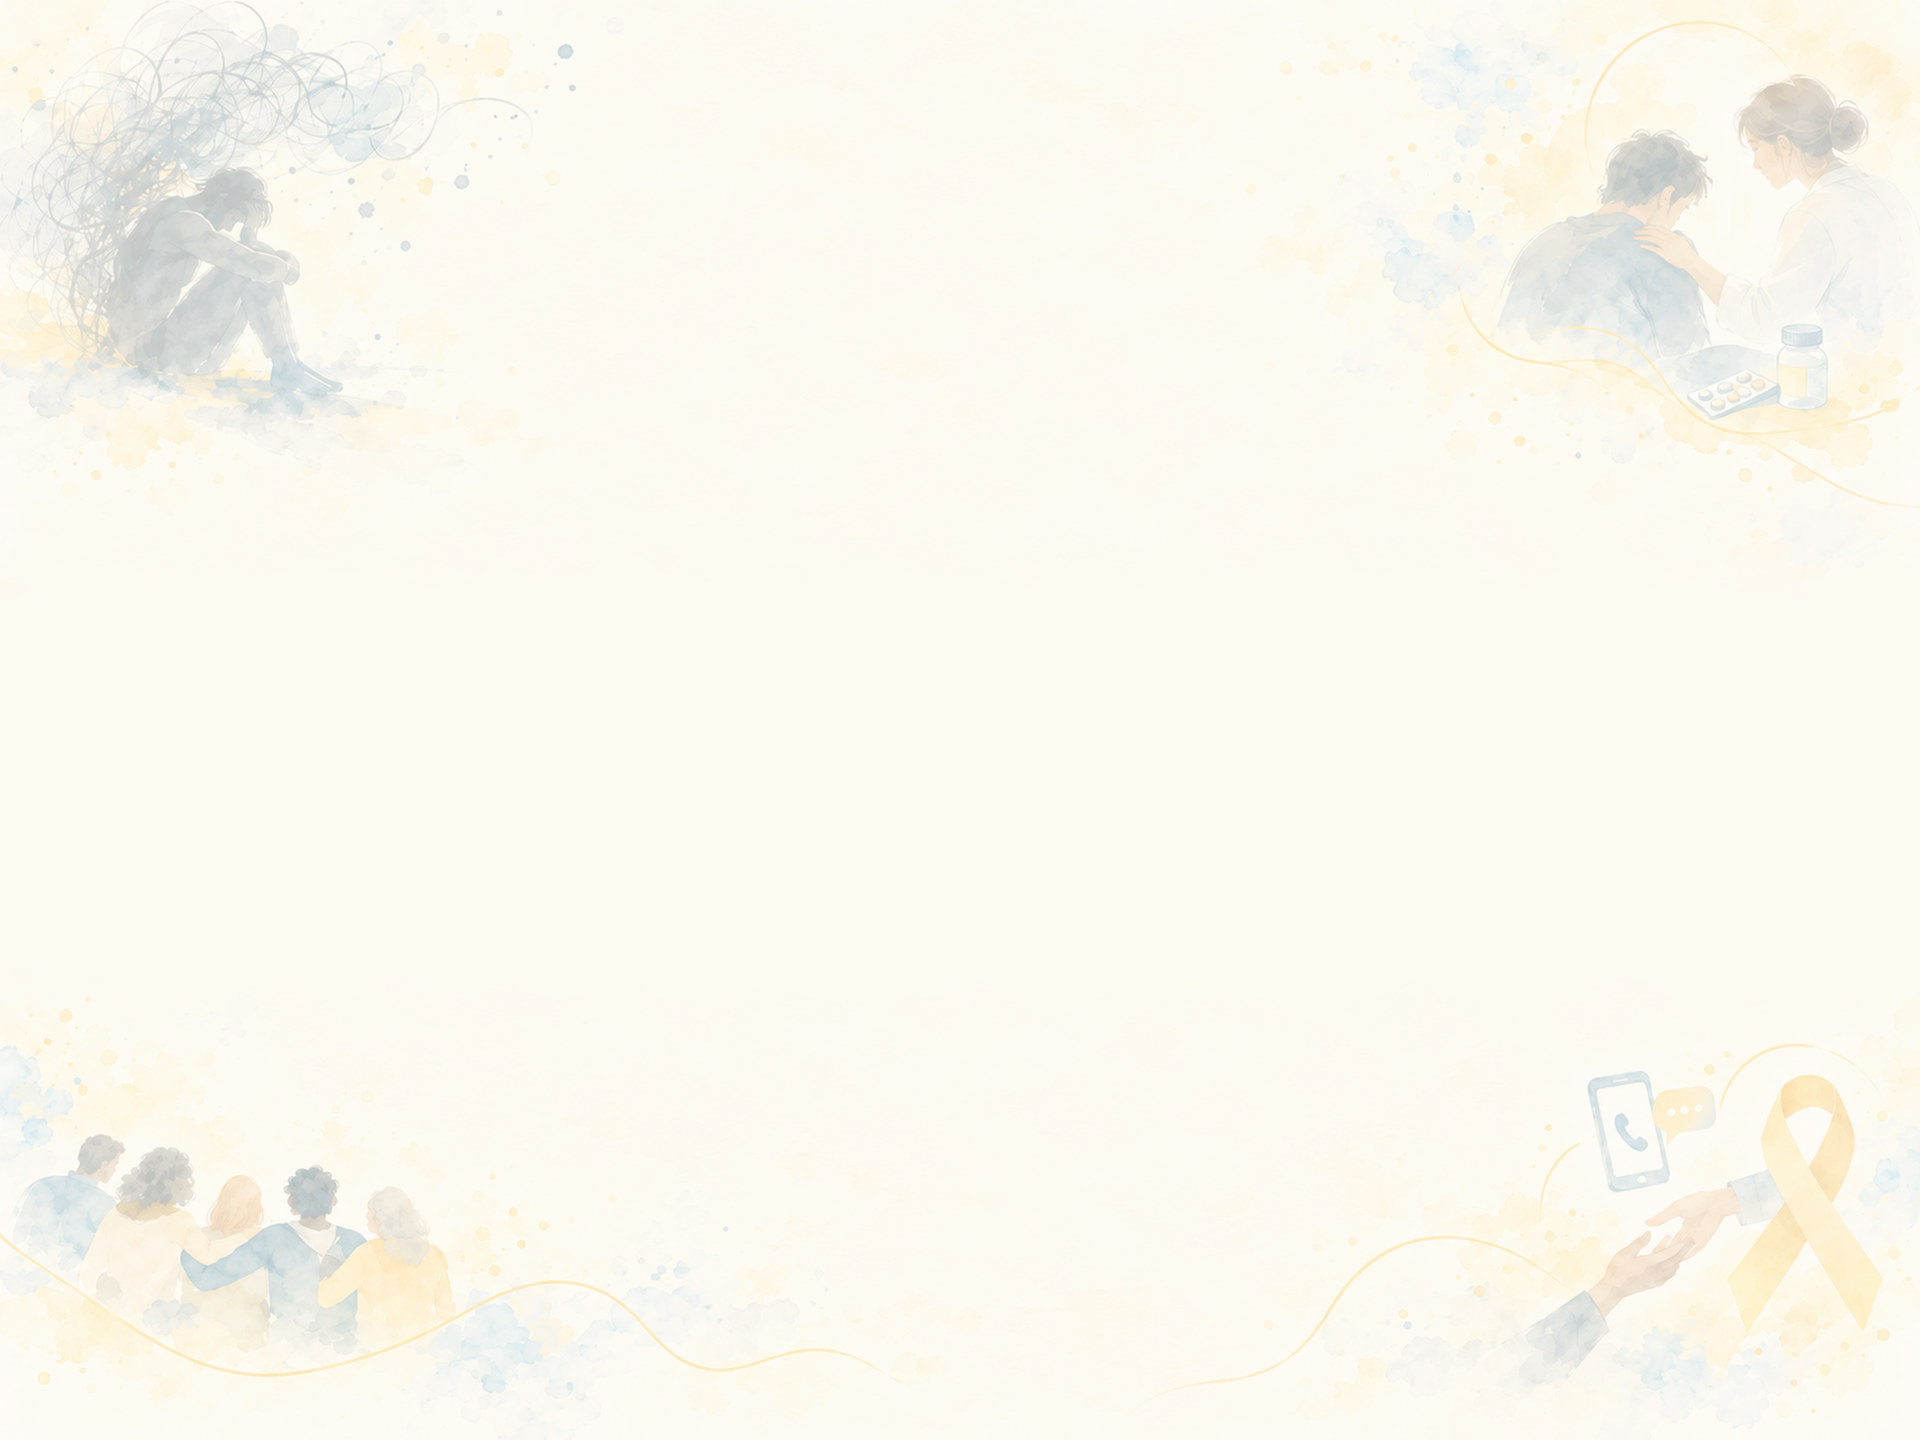
\includegraphics[width=\paperwidth,height=\paperheight]{ilustracoes/BACKGROUND.jpg}}%
  }{}
\fi

% --- Identificacao da apresentacao -------------------------------------------
\title[Risco de suic\'idio]{Risco de suic\'idio}
\subtitle{Avalia\c{c}\~ao e conduta}
\author[Prof. J. F. Musial]{Prof. Jo\~ao Frederico Musial}
\institute[Medicina | Campo Real]{Medicina | Campo Real}
\date[E3M40]{M\'odulo E3M40 \textbar{} 2026}


\begin{document}

% =============================================================================
% =============================================================================
% 00-abertura.tex - PARTE 0, abertura. Frames 01 a 03.
% =============================================================================

% ----------------------------------------------------------------- frame 01 --
% Capa. Unica excecao declarada de composicao: a ilustracao sangra de borda a
% borda e o texto ocupa a faixa central, que na arte e papel limpo. Os quatro
% cantos trazem, em sentido horario a partir do alto e a esquerda, o sofrimento
% isolado, o cuidado clinico, a rede que acolhe e o contato que se oferece, que
% e a propria cadeia da aula.
\begin{frame}[plain]
\CRar{0}
\begin{tikzpicture}[remember picture, overlay]
  \node[anchor=center, inner sep=0] at (current page.center) {%
    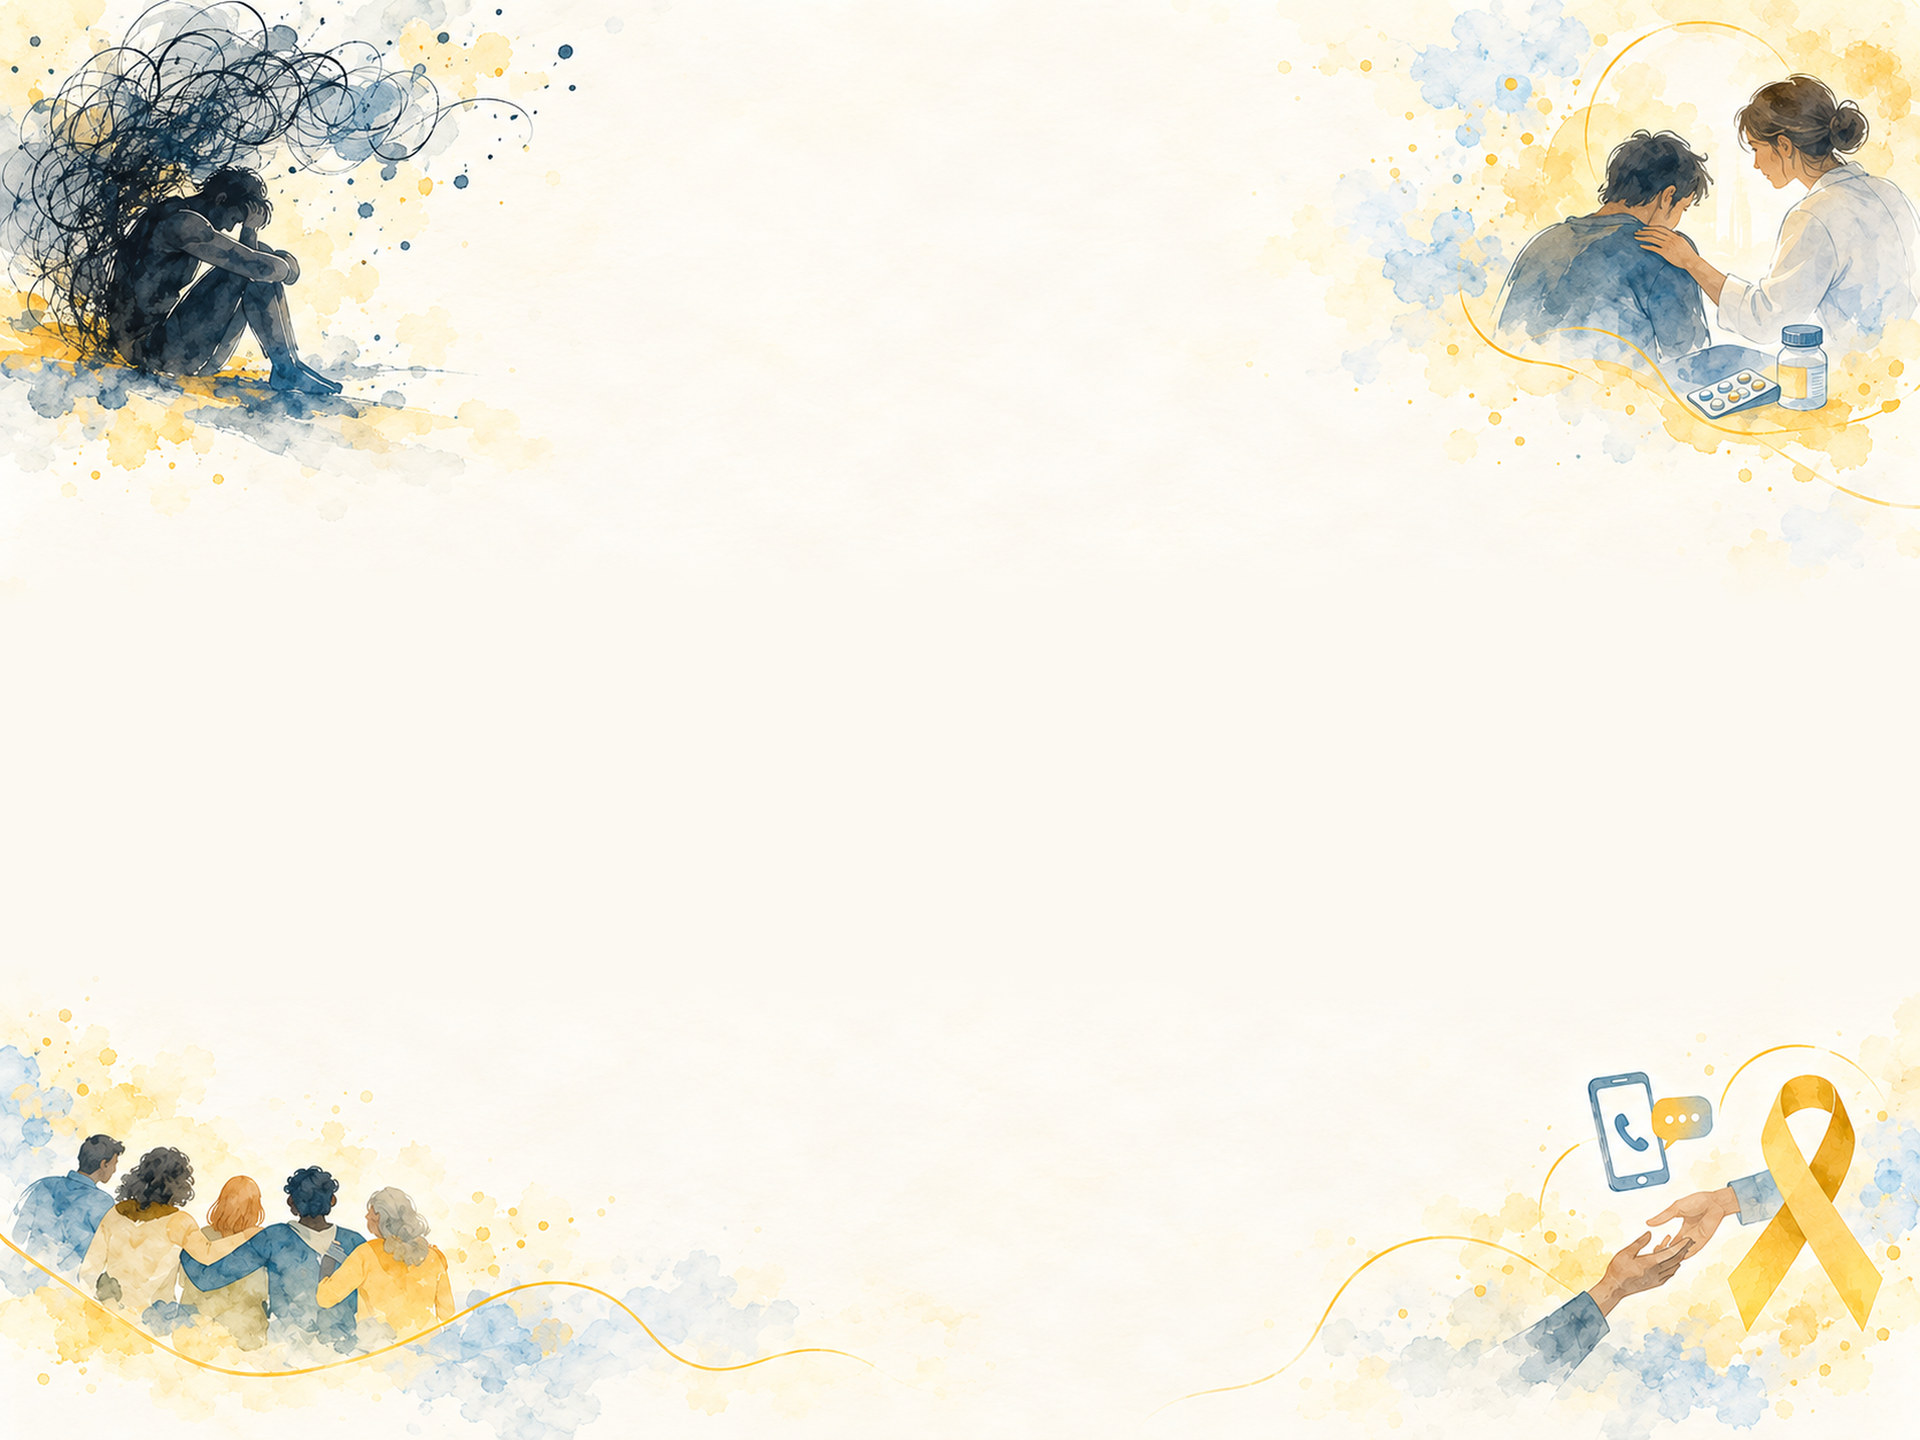
\includegraphics[width=\paperwidth, height=\paperheight]{ilustracoes/CAPA.jpg}};

  \node[anchor=center, align=center] at ($(current page.center)+(0,0.55cm)$) {%
    \begin{minipage}{8.2cm}\centering
      {\sffamily\bfseries\scriptsize\color{campobordo}%
       ATIVIDADE TE\'ORICO-PR\'ATICA}\\[0.30cm]
      {\sffamily\bfseries\LARGE\color{campoazul}Risco de suic\'idio}\\[0.14cm]
      {\sffamily\large\color{campoazul!75!black}avalia\c{c}\~ao e conduta}\\[0.34cm]
      {\color{campoamarelo!85!black}\rule{4.6cm}{1.6pt}}\\[0.30cm]
      {\sffamily\small\color{campografite}M\'odulo E3M40\\[0.05cm]
       Funcionalidade III, Cogni\c{c}\~ao e Humor}
    \end{minipage}};

  \node[anchor=south, align=center] at ($(current page.south)+(0,1.02cm)$) {%
    \begin{minipage}{7.0cm}\centering
      {\sffamily\footnotesize\color{campoazul!85!black}%
       \textbf{Prof. Jo\~ao Frederico Musial}}\\[0.06cm]
      {\sffamily\footnotesize\color{campografite}%
       Medicina \textbar{} Campo Real \textbar{} 2026}
    \end{minipage}};
\end{tikzpicture}
\end{frame}

% ----------------------------------------------------------------- frame 02 --
% Aviso de conteudo. Sobrio, sem dramatizacao, com saida garantida.
\begin{frame}{\ftit{\faHandHoldingHeart}{Antes de come\c{c}armos}}
\CRar{6}
\begin{caixaavaliar}{O que vamos discutir}
Esta aula trata de suic\'idio de forma direta, com falas de pacientes e com
decis\~oes cl\'inicas reais. N\~ao haver\'a imagem de m\'etodo, de cena nem de
les\~ao.
\end{caixaavaliar}

\CRvg
\begin{caixaproteger}{Voc\^e pode sair}
Se em algum momento voc\^e precisar se afastar, saia da sala. N\~ao \'e preciso
justificar, e isso n\~ao ser\'a registrado de nenhuma forma. Voltar depois
tamb\'em est\'a certo.
\end{caixaproteger}

\CRvg
\begin{center}
\begin{tikzpicture}
  \node[musialGreen, text width=9.2cm, font=\small] {%
    \faPhoneVolume~~\textbf{CVV 188}, liga\c{c}\~ao gratuita, 24 horas\\[2pt]
    \footnotesize O apoio ao estudante do Campo Real est\'a dispon\'ivel depois
    da aula. O docente tamb\'em est\'a.};
\end{tikzpicture}
\end{center}
\end{frame}

% ----------------------------------------------------------------- frame 03 --
% A pergunta da aula e a tese em duas linhas.
\begin{frame}{\ftit{\faQuestion}{A pergunta desta aula}}
\CRar{2.5}
\begin{center}
\begin{tikzpicture}
  \node[musialBlue, text width=9.0cm, font=\small, inner ysep=7pt] (p) {%
    \sffamily\bfseries \'E poss\'ivel construir seguran\c{c}a suficiente fora de
    um ambiente protegido neste momento?};
\end{tikzpicture}
\end{center}

\CRvg
\begin{caixaavaliar}{A tese}
O risco suicida \'e \avaliar{formula\c{c}\~ao cl\'inica din\^amica}, constru\'ida
pela intera\c{c}\~ao entre vulnerabilidades basais e modificadores proximais, e
n\~ao se reduz a escore nem a categoria. A conduta deve produzir
\proteger{seguran\c{c}a agora} e \proteger{continuidade depois}.
\end{caixaavaliar}

\CRvg
\begin{center}
\begin{tikzpicture}[node distance=0.20cm]
  \node[crnode={campoazul}{1.42cm}, font=\scriptsize, inner xsep=4pt] (a) {avaliar};
  \node[crnode={campoazul}{1.42cm}, font=\scriptsize, inner xsep=4pt, right=of a] (b) {formular};
  \node[crnode={campobordo}{1.42cm}, font=\scriptsize, inner xsep=4pt, right=of b] (c) {decidir};
  \node[crnode={campoverde}{1.70cm}, font=\scriptsize, inner xsep=4pt, right=of c] (d) {construir\\seguran\c{c}a};
  \node[crnode={campoverde}{1.70cm}, font=\scriptsize, inner xsep=4pt, right=of d] (e) {garantir\\continuidade};
  \draw[crseta=campoazul]  (a.east) -- (b.west);
  \draw[crseta=campoazul]  (b.east) -- (c.west);
  \draw[crseta=campobordo] (c.east) -- (d.west);
  \draw[crseta=campoverde] (d.east) -- (e.west);
\end{tikzpicture}
\end{center}

\mensagem{Ao final: o que, neste paciente, muda o que voc\^e far\'a nos
pr\'oximos 30 minutos?}
\end{frame}
        % frames 01 a 03
% =============================================================================
\section{O que estamos tentando entender}
% =============================================================================
% 01-fenomenologia.tex - PARTE 1, o que estamos tentando entender.
% Frames 04 a 08.
% =============================================================================

% ----------------------------------------------------------------- frame 04 --
% Primeiro frame de conteudo. Declara o recorte em uma linha e traz o mapa
% fenomenologico NAO linear, com relacoes bidirecionais.
\begin{frame}{\ftit{\faSitemap}{O que estamos tentando entender}}
\CRar{2.5}
{\footnotesize\sffamily\color{campografite}%
A prele\c{c}\~ao paralela do m\'odulo cobre o diagn\'ostico do epis\'odio
depressivo; esta ATP cobre a conduta e trata a suicidalidade como fen\^omeno
transdiagn\'ostico.\par}

\CRvg
\begin{center}
\begin{tikzpicture}[node distance=0.42cm and 0.60cm]
  \node[crnode={campoazul}{2.30cm}, font=\scriptsize]                 (pass) {idea\c{c}\~ao\\passiva};
  \node[crnode={campoazul}{2.30cm}, font=\scriptsize, right=of pass]  (ativ) {idea\c{c}\~ao\\ativa};
  \node[crnode={campoazul}{2.30cm}, font=\scriptsize, right=of ativ]  (inte) {inten\c{c}\~ao};
  \node[crnode={campoambar}{2.30cm}, font=\scriptsize, below=0.72cm of pass] (plan) {planejamento};
  \node[crnode={campoambar}{2.30cm}, font=\scriptsize, right=of plan] (prep) {comportamento\\preparat\'orio};
  \node[crnode={campobordo}{2.30cm}, font=\scriptsize, right=of prep] (tent) {tentativa};

  \draw[musialBi] (pass.east) -- (ativ.west);
  \draw[musialBi] (ativ.east) -- (inte.west);
  \draw[musialBi] (plan.east) -- (prep.west);
  \draw[musialBi] (prep.east) -- (tent.west);
  \draw[musialBi] (inte.south) -- (prep.north);
  \draw[musialBi] (ativ.south) -- (plan.north);
  \draw[musialBi, campobordo!80!black] (tent.north) to[out=60,in=0,looseness=1.5] (inte.east);
  \draw[musialBi] (plan.west) to[out=180,in=180,looseness=1.3] (pass.west);

  \node[crnode={campografite}{3.05cm}, font=\scriptsize, below=0.62cm of prep]
    (auto) {autoles\~ao sem inten\c{c}\~ao suicida\\[1pt]\scriptsize eixo paralelo};
  \draw[musialThin, dash pattern=on 2.4pt off 2pt] (auto.north) -- (prep.south);
\end{tikzpicture}
\end{center}

\mensagem{Esses fen\^omenos se relacionam nos dois sentidos. N\~ao s\~ao uma
escada obrigat\'oria.}
\end{frame}

% ----------------------------------------------------------------- frame 05 --
% A pirâmide de progressao como objeto de critica, e o eixo paralelo da autolesao.
\begin{frame}{\ftit{\faBan}{Duas leituras que atrapalham}}
\CRar{6}
\begin{columns}[onlytextwidth, t]
\begin{column}{0.47\textwidth}
\begin{caixaagir}{A escada que n\~ao existe}
Ningu\'em precisa passar por todos os degraus, na ordem, para chegar \`a
tentativa. Uma parte das tentativas ocorre em quem nunca planejou, e uma parte
de quem planeja durante anos nunca tenta.\par
\agir{Consequ\^encia:} a aus\^encia de um degrau anterior n\~ao tranquiliza.
\end{caixaagir}
\end{column}
\calha
\begin{column}{0.47\textwidth}
\begin{caixaavaliar}{A autoles\~ao no eixo ao lado}
A autoles\~ao sem inten\c{c}\~ao suicida tem fun\c{c}\~ao de regula\c{c}\~ao do
sofrimento, e n\~ao de morte. N\~ao \'e tentativa.\par
\avaliar{E ainda assim} \'e um dos marcadores mais consistentes de risco
futuro. As duas coisas s\~ao verdadeiras ao mesmo tempo.
\end{caixaavaliar}
\end{column}
\end{columns}

\CRvg
\begin{center}
\begin{tikzpicture}
  \node[crnode={campografite}{9.6cm}, font=\scriptsize] {%
    Dizer \fala{ele s\'o tem idea\c{c}\~ao passiva} e encerrar a\'i \'e usar um
    degrau como se fosse um progn\'ostico.};
\end{tikzpicture}
\end{center}
\end{frame}

% ----------------------------------------------------------------- frame 06 --
% Magnitude e tendencia. pgfplots. Apenas os dois pontos documentados.
\begin{frame}{\ftit{\faChartLine}{Magnitude e tend\^encia no Brasil}}
\CRar{4.6}
\begin{columns}[onlytextwidth, T]
\begin{column}{0.50\textwidth}
\begin{center}
\begin{tikzpicture}
\begin{axis}[
  width=5.4cm, height=4.2cm,
  ymin=0, ymax=9, xmin=2008.6, xmax=2022.4,
  xtick={2010,2021}, xticklabels={2010,2021},
  ytick={0,2,4,6,8},
  ylabel={\scriptsize \'obitos por 100 mil},
  y label style={font=\scriptsize, color=campografite},
  tick label style={font=\scriptsize, color=campografite},
  axis line style={campografite!55},
  grid=major, grid style={campografite!14, line width=0.3pt},
  every axis plot/.append style={line width=1.1pt}]
  \addplot[campoazul!85!black, mark=*, mark size=2.3pt,
           mark options={fill=campoazul!25, draw=campoazul!85!black}]
    coordinates {(2010,5.2) (2021,7.5)};
  \node[font=\scriptsize\sffamily, color=campoazul!85!black, anchor=south east]
    at (axis cs:2010,5.2) {5,2};
  \node[font=\scriptsize\sffamily, color=campoazul!85!black, anchor=south east]
    at (axis cs:2021,7.5) {7,5};
\end{axis}
\end{tikzpicture}
\end{center}
{\scriptsize\sffamily\color{campografite}\hspace{0.3cm}Dois pontos documentados.
A s\'erie intermedi\'aria n\~ao foi reconstru\'ida.\par}
\end{column}
\calha
\begin{column}{0.44\textwidth}
\begin{caixaavaliar}{2021, no Brasil}
\begin{itemc}
\item \avaliar{15.507} mortes por suic\'idio
\item \avaliar{114.159} notifica\c{c}\~oes de les\~ao autoprovocada
\item taxa de \avaliar{7,5} por 100 mil, \mudanca{42\% acima} da taxa de 2010
\end{itemc}
\end{caixaavaliar}
\CRvg
\begin{caixamudanca}{O que essa raz\~ao diz}
Para cada morte registrada h\'a cerca de sete notifica\c{c}\~oes de les\~ao
autoprovocada. Essas pessoas passam pelo servi\c{c}o.
\end{caixamudanca}
\end{column}
\end{columns}
\fonte{Minist\'erio da Sa\'ude, Boletim Epidemiol\'ogico v.\,55, n.\,4, 2024,
com dados do SIM e do SINAN.}
\end{frame}

% ----------------------------------------------------------------- frame 07 --
% Faixas etarias e sexo. Barras agrupadas, dado numericamente publicado.
\begin{frame}{\ftit{\faUsers}{Quem morre, por faixa et\'aria e sexo}}
\CRar{6}
\begin{center}
\begin{tikzpicture}
\begin{axis}[
  width=10.6cm, height=5.0cm,
  ybar=1.4pt, bar width=8.5pt,
  ymin=0, ymax=23, ytick={0,5,10,15,20},
  symbolic x coords={5 a 14,15 a 19,20 a 29,30 a 49,50 a 69,70 ou mais},
  xtick=data,
  ylabel={\scriptsize \'obitos por 100 mil, 2021},
  y label style={font=\scriptsize, color=campografite},
  tick label style={font=\scriptsize, color=campografite},
  axis line style={campografite!55},
  ymajorgrids, grid style={campografite!14, line width=0.3pt},
  legend style={font=\scriptsize\sffamily, draw=campografite!35, at={(0.015,0.98)},
                anchor=north west, legend columns=2, column sep=5pt},
  nodes near coords, nodes near coords style={font=\tiny\sffamily,
                                             color=campografite},
  every node near coord/.append style={/pgf/number format/.cd, fixed,
                                       precision=1, use comma}]
  \addplot[draw=campoazul!85!black, fill=campoazul!30,
           every node near coord/.append style={/tikz/.cd, yshift=5.5pt, xshift=-2.6pt}]
    coordinates {(5 a 14,0.7) (15 a 19,9.3) (20 a 29,14.6) (30 a 49,14.9)
                 (50 a 69,15.4) (70 ou mais,18.1)};
  \addplot[draw=camporoxo!80!black, fill=camporoxo!22,
           every node near coord/.append style={/tikz/.cd, xshift=2.6pt}]
    coordinates {(5 a 14,0.9) (15 a 19,4.5) (20 a 29,3.9) (30 a 49,3.8)
                 (50 a 69,3.8) (70 ou mais,2.9)};
  \legend{homens, mulheres}
\end{axis}
\end{tikzpicture}
\end{center}

\mensagem{A taxa mais alta est\'a nos homens com 70 anos ou mais. \'E a faixa que
o servi\c{c}o menos pergunta.}
\fonte{Minist\'erio da Sa\'ude, Boletim Epidemiol\'ogico v.\,55, n.\,4, 2024.}
\end{frame}

% ----------------------------------------------------------------- frame 08 --
% Contato previo com servicos. O argumento que sustenta toda a aula.
\begin{frame}{\ftit{\faUserMd}{Eles passam por n\'os antes}}
\CRar{6}
\begin{center}
\begin{tikzpicture}
\begin{axis}[
  width=9.55cm, height=4.10cm,
  xbar, bar width=11pt,
  xmin=0, xmax=100,
  symbolic y coords={smm, apm, sma, apa},
  ytick=data,
  yticklabels={{sa\'ude mental, no m\^es},
               {aten\c{c}\~ao prim\'aria, no m\^es},
               {sa\'ude mental, no ano},
               {aten\c{c}\~ao prim\'aria, no ano}},
  yticklabel style={font=\scriptsize, color=campografite, align=right},
  xlabel={\scriptsize \% das pessoas que morreram por suic\'idio},
  x label style={font=\scriptsize, color=campografite},
  tick label style={font=\scriptsize, color=campografite},
  axis line style={campografite!55},
  enlarge y limits=0.20,
  xmajorgrids, grid style={campografite!14, line width=0.3pt},
  nodes near coords, nodes near coords style={font=\tiny\sffamily,
                                              color=campografite, anchor=west,
                                              xshift=1.5pt},
  point meta=explicit symbolic]
  \addplot[draw=campoazul!85!black, fill=campoazul!30]
    coordinates {(20,smm)[20\%] (45,apm)[45\%]
                 (33,sma)[33\%] (75,apa)[75\%]};
\end{axis}
\end{tikzpicture}
\end{center}

\begin{caixaavaliar}{O que isso obriga}
A pessoa que morre por suic\'idio costuma ter estado diante de um m\'edico pouco
antes, e quase sempre de um m\'edico que n\~ao era psiquiatra. Em idosos, o
contato com a aten\c{c}\~ao prim\'aria no m\^es anterior \'e ainda mais
frequente do que em adultos jovens.
\end{caixaavaliar}

\fonte{Luoma, Martin e Pearson, \emph{Am J Psychiatry} 2002, revis\~ao de 40
estudos. \seloevidencia}
\end{frame}
   % frames 04 a 08
% =============================================================================
\section{Como perguntar}
% =============================================================================
% 02-entrevista.tex - PARTE 2, como perguntar. Frames 09 a 15.
% Frases LITERAIS na tela, nao parafrases.
% =============================================================================

% ----------------------------------------------------------------- frame 09 --
\begin{frame}{\ftit{\faCommentDots}{Perguntar n\~ao cria suicidalidade}}
\CRar{2.4}
\begin{caixaavaliar}{O receio e a evid\^encia}
O receio de que perguntar sobre suic\'idio possa induzir a ideia \'e comum e
n\~ao se sustenta. Revis\~ao da literatura publicada n\~ao encontrou, em
nenhum dos estudos revisados, aumento estatisticamente significativo de
idea\c{c}\~ao suicida entre os participantes que foram perguntados.
\end{caixaavaliar}

\CRvg
\begin{columns}[onlytextwidth, t]
\begin{column}{0.47\textwidth}
\begin{caixaproteger}{O que perguntar produz}
\begin{itemc}
\item nomeia o que o paciente n\~ao sabia como dizer
\item mostra que o assunto cabe nesta consulta
\item permite a pergunta seguinte
\end{itemc}
\end{caixaproteger}
\end{column}
\calha
\begin{column}{0.47\textwidth}
\begin{caixaagir}{O que n\~ao perguntar produz}
\begin{itemc}
\item um registro que diz apenas \fala{nega idea\c{c}\~ao}
\item uma alta que ningu\'em consegue justificar depois
\item a impress\~ao, no paciente, de que aquilo n\~ao se fala aqui
\end{itemc}
\end{caixaagir}
\end{column}
\end{columns}

\fonte{Dazzi, Gribble, Wessely e Fear, \emph{Psychol Med} 2014, revis\~ao em
formato de editorial. \seloevidencia}
\end{frame}

% ----------------------------------------------------------------- frame 10 --
\begin{frame}{\ftit{\faEye}{Reconhecer a pista}}
\CRar{2.6}
{\small Estas falas chegam ao pronto atendimento por outro motivo. Elas s\~ao a
abertura, e n\~ao a queixa.\par}

\CRvg
\begin{columns}[onlytextwidth, t]
\begin{column}{0.47\textwidth}
\begin{caixaavaliar}{O que o paciente diz}
\begin{itemc}
\item \fala{eu queria dormir e n\~ao acordar}
\item \fala{assim n\~ao d\'a mais}
\item \fala{eles ficariam melhor sem mim}
\item \fala{eu estou s\'o cansado, doutor}
\item \fala{n\~ao sei quanto tempo eu aguento}
\end{itemc}
\end{caixaavaliar}
\end{column}
\calha
\begin{column}{0.47\textwidth}
\begin{caixamudanca}{O que a fam\'ilia diz}
\begin{itemc}
\item \fala{ele deu as coisas dele}
\item \fala{ela ficou estranhamente calma}
\item \fala{ele se despediu de um jeito esquisito}
\item \fala{ela parou de atender o telefone}
\item \fala{ele acertou tudo o que estava pendente}
\end{itemc}
\end{caixamudanca}
\end{column}
\end{columns}

\mensagem{Toda pista reconhecida obriga \`a pergunta seguinte. Reconhecer e n\~ao
perguntar \'e pior do que n\~ao ter reconhecido.}
\end{frame}

% ----------------------------------------------------------------- frame 11 --
\begin{frame}{\ftit{\faComments}{A frase de transi\c{c}\~ao}}
\CRar{4.3}
{\footnotesize Esta \'e a frase. N\~ao \'e exemplo do que dizer, \'e o que se
diz.\par}

\CRvg
\begin{center}
\begin{tikzpicture}
  \node[musialBlue, text width=9.4cm, font=\footnotesize, inner ysep=6pt] {%
    \itshape\guillemotleft Pelo que voc\^e est\'a me contando, esse sofrimento
    est\'a bem pesado. Quando as pessoas chegam assim, \`as vezes pensam em
    morrer. Voc\^e tem tido esses pensamentos?\guillemotright};
\end{tikzpicture}
\end{center}

\CRvg
\begin{columns}[onlytextwidth, t]
\begin{column}{0.47\textwidth}
\begin{caixaproteger}{Por que funciona}
Nomeia o sofrimento antes de perguntar, universaliza sem banalizar, e faz uma
pergunta fechada que o paciente consegue responder com uma palavra.
\end{caixaproteger}
\end{column}
\calha
\begin{column}{0.47\textwidth}
\begin{caixaagir}{O que n\~ao dizer}
\fala{Voc\^e n\~ao est\'a pensando em fazer besteira, est\'a?}\par
\vspace{0.06cm}
A pergunta j\'a traz a resposta esperada.
\end{caixaagir}
\end{column}
\end{columns}
\end{frame}

% ----------------------------------------------------------------- frame 12 --
% Roteiro de perguntas. Uma das tres tabelas autorizadas na aula.
\begin{frame}{\ftit{\faSearch}{Caracterizar a idea\c{c}\~ao}}
\CRar{2.2}
\begin{CRtabela}
\begin{center}
\begin{tabular}{E P{4.05cm} P{4.05cm}}
\toprule
\rowcolor{campoazul!10}
\textbf{O que caracterizar} & \textbf{Como perguntar} & \textbf{O que muda} \\
\midrule
existe & \fala{voc\^e tem tido esses pensamentos?} & abre ou fecha toda a
sequ\^encia \\
frequ\^encia & \fala{quantas vezes, num dia como o de ontem?} & separa o
epis\'odico do cont\'inuo \\
dura\c{c}\~ao & \fala{quando vem, fica quanto tempo?} & minutos e horas pedem
condutas diferentes \\
intrusividade & \fala{ele vem sozinho ou voc\^e o chama?} & pensamento que
invade cansa e desgasta \\
capacidade de afastar & \fala{quando vem, voc\^e consegue empurrar? o que
ajuda?} & \'e aqui que mora o plano de seguran\c{c}a \\
\bottomrule
\end{tabular}
\end{center}
\end{CRtabela}

\mensagem{A \'ultima linha \'e a mais \'util das cinco, e \'e a que quase
ningu\'em pergunta.}
\end{frame}

% ----------------------------------------------------------------- frame 13 --
\begin{frame}{\ftit{\faRoute}{Inten\c{c}\~ao, plano e prepara\c{c}\~ao}}
\CRar{6}
\begin{center}
\begin{tikzpicture}[node distance=0.34cm]
  \node[crnode={campoazul}{2.55cm}, font=\scriptsize] (i) {\textbf{inten\c{c}\~ao}\\[1pt]
    \fala{voc\^e quer morrer ou quer que isso pare?}};
  \node[crnode={campoambar}{2.55cm}, font=\scriptsize, right=of i] (p) {\textbf{plano}\\[1pt]
    \fala{voc\^e chegou a pensar em como faria?}};
  \node[crnode={campoambar}{2.55cm}, font=\scriptsize, right=of p] (r) {\textbf{prepara\c{c}\~ao}\\[1pt]
    \fala{voc\^e chegou a fazer alguma coisa nessa dire\c{c}\~ao?}};
  \draw[crseta=campoazul] (i.east) -- (p.west);
  \draw[crseta=campoambar] (p.east) -- (r.west);
\end{tikzpicture}
\end{center}

\CRvg
\begin{columns}[onlytextwidth, t]
\begin{column}{0.47\textwidth}
\begin{caixaavaliar}{A pergunta que falta}
Depois de \fala{fez alguma coisa?}, vem \fala{mesmo que depois voc\^e tenha
desistido}. \'E essa segunda metade que autoriza o paciente a contar o ato
interrompido.
\end{caixaavaliar}
\end{column}
\calha
\begin{column}{0.47\textwidth}
\begin{caixaagir}{O que n\~ao entra na tela nem na pergunta}
N\~ao se pergunta detalhe de m\'etodo por curiosidade cl\'inica, e n\~ao se
compara letalidade diante do paciente. O que importa \'e a exist\^encia do
acesso e a possibilidade de restringi-lo.
\end{caixaagir}
\end{column}
\end{columns}
\end{frame}

% ----------------------------------------------------------------- frame 14 --
\begin{frame}{\ftit{\faClock}{Comportamento e temporalidade}}
\CRar{1.3}
\begin{caixamudanca}{A pergunta que organiza o tempo}
\fala{O que mudou nas \'ultimas horas? E nos \'ultimos dias?}
\end{caixamudanca}

\CRvg
\begin{center}
\begin{tikzpicture}[node distance=0.30cm]
  \node[crnode={campografite}{2.15cm}, font=\scriptsize] (v) {meses e anos\\[1pt]
    \scriptsize vulnerabilidade};
  \node[crnode={campoambar}{2.15cm}, font=\scriptsize, right=of v] (s) {\'ultimas semanas\\[1pt]
    \scriptsize deteriora\c{c}\~ao};
  \node[crnode={campoambar}{2.15cm}, font=\scriptsize, right=of s] (d) {\'ultimos dias\\[1pt]
    \scriptsize prepara\c{c}\~ao};
  \node[crnode={campobordo}{2.15cm}, font=\scriptsize, right=of d] (h) {\'ultimas horas\\[1pt]
    \scriptsize decis\~ao de hoje};
  \draw[musialThin] (v.east) -- (s.west);
  \draw[crseta=campoambar] (s.east) -- (d.west);
  \draw[crseta=campobordo] (d.east) -- (h.west);
\end{tikzpicture}
\end{center}

\CRvg
\begin{columns}[onlytextwidth, t]
\begin{column}{0.47\textwidth}
\begin{caixaavaliar}{O que perguntar do comportamento}
\begin{itemc}
\item o que fez, n\~ao s\'o o que pensou
\item o que interrompeu o ato, quando houve
\item o que estava acontecendo naquela hora
\end{itemc}
\end{caixaavaliar}
\end{column}
\calha
\begin{column}{0.47\textwidth}
\begin{caixamudanca}{Mudan\c{c}as que pesam}
\begin{itemc}
\item sono que encurtou de repente
\item retraimento que apertou nos \'ultimos dias
\item algo resolvido ou acertado sem explica\c{c}\~ao
\end{itemc}
\end{caixamudanca}
\end{column}
\end{columns}
\end{frame}

% ----------------------------------------------------------------- frame 15 --
\begin{frame}{\ftit{\faBolt}{O que modifica a seguran\c{c}a agora}}
\CRar{6}
\begin{center}
\begin{tikzpicture}[node distance=0.26cm and 0.30cm]
  \node[musialCenter, minimum size=1.95cm, font=\scriptsize\bfseries\sffamily] (c)
    {modificadores\\proximais};

  \node[crnode={campoambar}{1.85cm}, font=\scriptsize, above left=0.60cm and 0.75cm of c] (subs) {subst\^ancias};
  \node[crnode={campoambar}{1.85cm}, font=\scriptsize, above=0.60cm of c] (agit) {agita\c{c}\~ao};
  \node[crnode={campoambar}{1.85cm}, font=\scriptsize, above right=0.60cm and 0.75cm of c] (ins) {ins\^onia};
  \node[crnode={campobordo}{1.85cm}, font=\scriptsize, left=0.80cm of c] (psic) {psicose};
  \node[crnode={campobordo}{1.85cm}, font=\scriptsize, right=0.80cm of c] (imp) {impulsividade};
  \node[crnode={campoazul}{1.85cm}, font=\scriptsize, below left=0.60cm and 0.75cm of c] (perd) {perdas recentes};
  \node[crnode={campoverde}{1.85cm}, font=\scriptsize, below=0.60cm of c] (rede) {rede dispon\'ivel};
  \node[crnode={campoverde}{1.85cm}, font=\scriptsize, below right=0.60cm and 0.75cm of c] (colab) {capacidade de colaborar};

  \draw[musialThin] (subs.south east) -- (c.north west);
  \draw[musialThin] (agit.south) -- (c.north);
  \draw[musialThin] (ins.south west) -- (c.north east);
  \draw[musialThin] (psic.east) -- (c.west);
  \draw[musialThin] (imp.west) -- (c.east);
  \draw[musialThin] (perd.north east) -- (c.south west);
  \draw[musialThin] (rede.north) -- (c.south);
  \draw[musialThin] (colab.north west) -- (c.south east);
\end{tikzpicture}
\end{center}

\mensagem{Supervis\~ao dispon\'ivel e capacidade de colaborar s\~ao
modificadores, e n\~ao detalhe de execu\c{c}\~ao do plano.}
\end{frame}
      % frames 09 a 15
% =============================================================================
\section{Como formular}
% =============================================================================
% 03-formulacao.tex - PARTE 3, como formular. Frames 16 a 20.
% A matriz comum em tela unica e depois desdobrada.
% =============================================================================

% ----------------------------------------------------------------- frame 16 --
% A MATRIZ COMUM, tela unica. Todos os frames seguintes desdobram esta.
\begin{frame}{\ftit{\faClipboardList}{A matriz da formula\c{c}\~ao}}
\CRar{6}
\begin{center}
\begin{tikzpicture}
  \node[crnode={campografite}{1.95cm}, font=\scriptsize, inner xsep=4pt,
        minimum height=1.05cm] (v) at (0,0) {vulnerabilidades\\basais};
  \node[font=\footnotesize\bfseries\color{campografite},
        right=0.09cm of v] (m1) {+};
  \node[crnode={campoambar}{1.60cm}, font=\scriptsize, inner xsep=4pt,
        minimum height=1.05cm, right=0.09cm of m1] (p) {modificadores\\proximais};
  \node[font=\footnotesize\bfseries\color{campografite},
        right=0.09cm of p] (m2) {+};
  \node[crnode={campoazul}{1.60cm}, font=\scriptsize, inner xsep=4pt,
        minimum height=1.05cm, right=0.09cm of m2] (s) {suicidalidade\\atual};
  \node[font=\footnotesize\bfseries\color{campografite},
        right=0.09cm of s] (m3) {+};
  \node[crnode={campobordo}{1.60cm}, font=\scriptsize, inner xsep=4pt,
        minimum height=1.05cm, right=0.09cm of m3] (a) {acesso\\a meios};

  \node[crnode={campoverde}{4.00cm}, font=\scriptsize, inner xsep=4pt,
        minimum height=0.78cm] (c) at ($(v.south)!0.5!(p.south) + (0,-1.05)$)
    {capacidade de construir seguran\c{c}a};
  \node[crnode={campoazul}{2.95cm}, font=\small, inner xsep=4pt,
        minimum height=0.78cm] (f) at ($(s.south)!0.5!(a.south) + (0.25,-1.05)$)
    {\textbf{formula\c{c}\~ao}};

  \draw[musialThin] (v.south) |- ($(c.north)+(0,0.28)$) -- (c.north);
  \draw[musialThin] (p.south) -- ($(p.south)+(0,-0.28)$) -- (c.north);
  \draw[crseta=campoazul]  (s.south) -- ($(s.south)+(0,-0.28)$) -- (f.north);
  \draw[crseta=campobordo] (a.south) |- ($(f.north)+(0,0.28)$) -- (f.north);
  \draw[crseta=campoverde] (c.east) -- (f.west);
\end{tikzpicture}
\end{center}

\CRvg
\begin{center}
\begin{tikzpicture}
  \node[musialBlue, text width=9.3cm, font=\small, inner ysep=7pt] {%
    \sffamily\bfseries \'E poss\'ivel construir seguran\c{c}a suficiente fora de
    um ambiente protegido neste momento?};
\end{tikzpicture}
\end{center}

\mensagem{A sa\'ida da matriz \'e uma pergunta que se responde com conduta, e
n\~ao uma etiqueta.}
\end{frame}

% ----------------------------------------------------------------- frame 17 --
\begin{frame}{\ftit{\faHourglassHalf}{Vulnerabilidades basais e modificadores proximais}}
\CRar{2}
\begin{columns}[onlytextwidth, t]
\begin{column}{0.47\textwidth}
\begin{caixanorma}{Vulnerabilidades basais}
O que este paciente carrega h\'a meses ou anos.
\begin{itemc}
\item transtorno mental em curso
\item tentativa pr\'evia, o preditor isolado mais forte
\item autoles\~ao recorrente
\item doen\c{c}a dolorosa ou incapacitante
\item isolamento e perda de papel social
\end{itemc}
\end{caixanorma}
\end{column}
\calha
\begin{column}{0.47\textwidth}
\begin{caixamudanca}{Modificadores proximais}
O que est\'a diferente nesta semana e nesta noite.
\begin{itemc}
\item intoxica\c{c}\~ao, agita\c{c}\~ao, ins\^onia
\item psicose e impulsividade
\item perda, humilha\c{c}\~ao, ruptura recente
\item mudan\c{c}a de tratamento ou alta recente
\item rede que deixou de estar dispon\'ivel
\end{itemc}
\end{caixamudanca}
\end{column}
\end{columns}

\mensagem{A vulnerabilidade explica por que este paciente, e n\~ao outro. O
modificador explica por que hoje, e n\~ao no m\^es passado.}
\end{frame}

% ----------------------------------------------------------------- frame 18 --
\begin{frame}{\ftit{\faKey}{Suicidalidade atual e acesso a meios}}
\CRar{6}
\begin{columns}[onlytextwidth, t]
\begin{column}{0.47\textwidth}
\begin{caixaavaliar}{Suicidalidade atual}
O que foi caracterizado na entrevista, em vez de resumido em uma palavra:
frequ\^encia, dura\c{c}\~ao, intrusividade, capacidade de afastar,
inten\c{c}\~ao, plano e prepara\c{c}\~ao, com a data do que houve.
\end{caixaavaliar}
\end{column}
\calha
\begin{column}{0.47\textwidth}
\begin{caixaagir}{Acesso a meios}
Tr\^es perguntas, e nenhuma sobre m\'etodo:
\begin{itemc}
\item existe acesso agora?
\item \'e concretamente poss\'ivel restringir?
\item quem da rede participa dessa restri\c{c}\~ao?
\end{itemc}
\end{caixaagir}
\end{column}
\end{columns}

\CRvg
\begin{center}
\begin{tikzpicture}
  \node[crnode={campografite}{9.5cm}, font=\scriptsize] {%
    A pergunta sobre arma de fogo na resid\^encia \'e obrigat\'oria e quase nunca
    aparece no registro. A aus\^encia dela \'e a falha mais comum destes
    atendimentos.};
\end{tikzpicture}
\end{center}
\end{frame}

% ----------------------------------------------------------------- frame 19 --
\begin{frame}{\ftit{\faHandsHelping}{Capacidade de construir seguran\c{c}a}}
\CRar{3.3}
{\small \'E o elemento que os outros quatro n\~ao mostram, e o que mais muda a
conduta.\par}

\CRvg
\begin{columns}[onlytextwidth, t]
\begin{column}{0.47\textwidth}
\begin{caixaproteger}{Sustenta o plano}
\begin{itemc}
\item comunica o que sente a algu\'em
\item aceita que a rede seja acionada
\item pactua o que far\'a se piorar
\item consegue reduzir o acesso hoje
\item tem quem permane\c{c}a com ele
\end{itemc}
\end{caixaproteger}
\end{column}
\calha
\begin{column}{0.47\textwidth}
\begin{caixaagir}{N\~ao sustenta o plano}
\begin{itemc}
\item oculta a situa\c{c}\~ao da fam\'ilia
\item recusa a participa\c{c}\~ao da rede
\item n\~ao consegue pactuar nada concreto
\item n\~ao colabora por psicose ou intoxica\c{c}\~ao
\item tem rede que existe e n\~ao sustenta
\end{itemc}
\end{caixaagir}
\end{column}
\end{columns}

\mensagem{Rede dispon\'ivel n\~ao \'e o mesmo que supervis\~ao poss\'ivel.
Pergunte o que aquela pessoa consegue fazer, e at\'e quando.}
\end{frame}

% ----------------------------------------------------------------- frame 20 --
% A critica ao semaforo. O unico lugar em que baixo, moderado e alto aparecem.
\begin{frame}{\ftit{\faTimes}{O que a matriz substitui}}
\CRar{4.6}
\begin{center}
\begin{tikzpicture}[node distance=0.22cm]
  \node[crnode={campografite}{1.38cm}, font=\scriptsize, inner xsep=4pt] (b) {baixo};
  \node[crnode={campografite}{1.38cm}, font=\scriptsize, inner xsep=4pt, right=of b] (m) {moderado};
  \node[crnode={campografite}{1.38cm}, font=\scriptsize, inner xsep=4pt, right=of m] (a) {alto};
  \node[font=\large\color{campobordo}, right=0.26cm of a] (x) {\faTimes};
  \node[crnode={campoazul}{3.30cm}, font=\scriptsize, inner xsep=4pt, right=0.26cm of x] (q)
    {\'E poss\'ivel construir seguran\c{c}a fora daqui agora?};
\end{tikzpicture}
\end{center}

\CRvg
\begin{caixaagir}{Por que o sem\'aforo n\~ao resolve}
A categoria n\~ao diz o que fazer. Dois pacientes classificados como risco
moderado podem exigir condutas opostas, e a classifica\c{c}\~ao n\~ao registra
nem o que sustenta a decis\~ao nem o que precisaria mudar para invert\^e-la.
Escalas ajudam a n\~ao esquecer perguntas e n\~ao decidem conduta.
\end{caixaagir}

\CRvg
\begin{caixaproteger}{O que a pergunta operacional entrega}
Uma resposta que j\'a \'e conduta, com as duas sa\'idas explicitadas, e um
registro que permite reconstruir depois por que a decis\~ao foi aquela.
\end{caixaproteger}
\end{frame}
      % frames 16 a 20
% =============================================================================
% 03b-contextos.tex - PARTE 3B, contextos que a matriz nao resolve sozinha.
% Frames 21 e 22. Gabarito fixo: macro unica \quadroDx, geometria identica,
% dois quadros por frame, nenhuma revisao do diagnostico.
%
% Estes dois frames sao obrigatorios. Sem eles o recorte transdiagnostico e
% anunciado e nao entregue, porque os seis casos da atividade nao cobrem
% nenhum destes quatro contextos.
% =============================================================================

% ----------------------------------------------------------------- frame 21 --
\begin{frame}{\ftit{\faUsers}{Contextos que a matriz n\~ao resolve sozinha, I}}
\CRar{0}
\begin{columns}[onlytextwidth, T]
\begin{column}{0.478\textwidth}
\quadroDx{Pessoa idosa}
{Inten\c{c}\~ao mais determinada, menos tentativas e maior letalidade por
tentativa. Doen\c{c}a dolorosa ou incapacitante, perda de autonomia, luto
recente e isolamento.}
{Manejo agressivo da dor e da comorbidade. Envolvimento expl\'icito do
cuidador. Revis\~ao do que est\'a guardado em casa.}
{Normalizar a desesperan\c{c}a como coisa da idade.}
\end{column}
\calha
\begin{column}{0.478\textwidth}
\quadroDx{Adolescente}
{Cont\'agio e efeito de exposi\c{c}\~ao. Humilha\c{c}\~ao, ruptura e
exposi\c{c}\~ao digital. Impulsividade pr\'opria da faixa.}
{Parceria com o respons\'avel, com o adolescente sabendo o que ser\'a dito.
Dever de comunica\c{c}\~ao ao Conselho Tutelar quando couber.}
{Prometer sigilo absoluto antes de saber o que ser\'a contado.}
\end{column}
\end{columns}
\end{frame}

% ----------------------------------------------------------------- frame 22 --
\begin{frame}{\ftit{\faUsers}{Contextos que a matriz n\~ao resolve sozinha, II}}
\CRar{0}
\begin{columns}[onlytextwidth, T]
\begin{column}{0.478\textwidth}
\quadroDx{Transtorno alimentar}
{Na anorexia nervosa, parcela relevante da mortalidade \'e por suic\'idio, e
n\~ao por complica\c{c}\~ao nutricional. Desesperan\c{c}a e vergonha
sustentadas por anos.}
{Perguntar sobre idea\c{c}\~ao em uma consulta que tende a girar s\'o em torno
de peso e de exame laboratorial.}
{Reduzir a avalia\c{c}\~ao ao risco cl\'inico nutricional.}
\end{column}
\calha
\begin{column}{0.478\textwidth}
\quadroDx{Crise psicossocial}
{Perda, viol\^encia, humilha\c{c}\~ao, problema jur\'idico ou financeiro, sem
transtorno estabelecido. Risco real e frequentemente transit\'orio.}
{A conduta \'e companhia e restri\c{c}\~ao de acesso, com reavalia\c{c}\~ao
pr\'oxima enquanto a crise passa.}
{Prescrever no lugar de organizar prote\c{c}\~ao.}
\end{column}
\end{columns}
\end{frame}
      % frames 21 a 22
% =============================================================================
\section{O que fazer agora}
% =============================================================================
% 04-conduta.tex - PARTE 4, o que fazer agora. Frames 23 a 29.
% Farmacologia sempre em roxo.
% =============================================================================

% ----------------------------------------------------------------- frame 23 --
\begin{frame}{\ftit{\faKey}{Restri\c{c}\~ao de acesso a meios}}
\CRar{3}
\begin{center}
\begin{tikzpicture}
  \node[musialGreen, text width=9.4cm, font=\footnotesize, inner ysep=6pt] {%
    \itshape\guillemotleft Eu preciso conversar com voc\^es dois sobre deixar a
    casa mais segura nos pr\'oximos dias. N\~ao \'e desconfian\c{c}a. \'E que,
    quando aperta, a dist\^ancia at\'e a coisa faz diferen\c{c}a. O que a gente
    consegue tirar de casa hoje, e quem fica respons\'avel?\guillemotright};
\end{tikzpicture}
\end{center}

\CRvg
\begin{columns}[onlytextwidth, t]
\begin{column}{0.47\textwidth}
\begin{caixaproteger}{O que a conversa precisa produzir}
\begin{itemc}
\item o que sai de casa, nomeado
\item quem retira e para onde vai
\item at\'e quando fica assim
\item quem confere que foi feito
\end{itemc}
\end{caixaproteger}
\end{column}
\calha
\begin{column}{0.47\textwidth}
\begin{caixaagir}{O que invalida a medida}
\begin{itemc}
\item combinar s\'o com o paciente, e n\~ao com quem executa
\item deixar sem prazo e sem respons\'avel
\item esquecer a arma de fogo
\item n\~ao conferir depois
\end{itemc}
\end{caixaagir}
\end{column}
\end{columns}
\end{frame}

% ----------------------------------------------------------------- frame 24 --
\begin{frame}{\ftit{\faLifeRing}{Plano de seguran\c{c}a}}
\CRar{2.7}
\begin{columns}[onlytextwidth, T]
\begin{column}{0.50\textwidth}
\begin{center}
\begin{tikzpicture}[node distance=0.20cm]
  \node[crnode={campoambar}{3.55cm}, font=\scriptsize, inner ysep=3pt] (a)
    {\textbf{1.} sinais de alerta dele};
  \node[crnode={campoverde}{3.55cm}, font=\scriptsize, inner ysep=3pt,
        below=of a] (b) {\textbf{2.} estrat\'egias que ele j\'a usa};
  \node[crnode={campoverde}{3.55cm}, font=\scriptsize, inner ysep=3pt,
        below=of b] (c) {\textbf{3.} pessoas e ambientes que ajudam};
  \node[crnode={campoverde}{3.55cm}, font=\scriptsize, inner ysep=3pt,
        below=of c] (d) {\textbf{4.} quem pode ser acionado};
  \node[crnode={campoverde}{3.55cm}, font=\scriptsize, inner ysep=3pt,
        below=of d] (e) {\textbf{5.} servi\c{c}os e profissionais};
  \node[crnode={campobordo}{3.55cm}, font=\scriptsize, inner ysep=3pt,
        below=of e] (f) {\textbf{6.} redu\c{c}\~ao do acesso};
  \draw[crseta=campoverde] (a.south) -- (b.north);
  \draw[crseta=campoverde] (b.south) -- (c.north);
  \draw[crseta=campoverde] (c.south) -- (d.north);
  \draw[crseta=campoverde] (d.south) -- (e.north);
  \draw[crseta=campobordo] (e.south) -- (f.north);
\end{tikzpicture}
\end{center}
\end{column}
\calha
\begin{column}{0.44\textwidth}
\begin{caixaproteger}{N\~ao \'e contrato de n\~ao suic\'idio}
O contrato pede uma promessa e protege o servi\c{c}o. O plano descreve o que a
pessoa faz, na ordem, quando o pensamento aperta, e protege a pessoa. O
contrato n\~ao tem sustenta\c{c}\~ao e n\~ao substitui o plano.
\end{caixaproteger}
\CRvg
\begin{caixaproteger}{Escrito com ele}
Nas palavras dele, no celular dele, com os nomes e os n\'umeros preenchidos
ainda na consulta.
\end{caixaproteger}
\end{column}
\end{columns}

\fonte{Com contato de seguimento, 45\% menos comportamento suicida em seis meses.
Stanley et al., \emph{JAMA Psychiatry} 2018. \seloevidencia}
\end{frame}

% ----------------------------------------------------------------- frame 25 --
\begin{frame}{\ftit{\faStethoscope}{Tratar a crise e tratar a base}}
\CRar{1.5}
{\small O erro mais comum desta etapa \'e reduzir tudo ao antidepressivo e
deixar sem tratamento o que est\'a produzindo o risco hoje.\par}

\CRvg
\begin{columns}[onlytextwidth, t]
\begin{column}{0.47\textwidth}
\begin{caixamudanca}{O que tratar agora}
\begin{itemc}
\item intoxica\c{c}\~ao em curso
\item priva\c{c}\~ao de sono
\item dor n\~ao controlada
\item agita\c{c}\~ao
\item psicose
\item a crise psicossocial que precipitou
\end{itemc}
\end{caixamudanca}
\end{column}
\calha
\begin{column}{0.47\textwidth}
\begin{caixaproteger}{O que tratar em seguida}
\begin{itemc}
\item a condi\c{c}\~ao de base, com o esquema correto para ela
\item o que est\'a mal tratado ou sem ades\~ao
\item o que mudou de tratamento h\'a pouco
\item os fatores modific\'aveis que a fam\'ilia consegue sustentar
\end{itemc}
\end{caixaproteger}
\end{column}
\end{columns}

\mensagem{Cada fator modific\'avel tratado hoje \'e um modificador proximal a
menos na formula\c{c}\~ao de amanh\~a.}
\end{frame}

% ----------------------------------------------------------------- frame 26 --
\begin{frame}{\ftit{\faPills}{Fam\'ilia do f\'armaco e seguran\c{c}a da prescri\c{c}\~ao}}
\CRar{4.7}
\begin{caixafarmaco}{Seguran\c{c}a em superdosagem}
Perfis diferem quanto ao que acontece em ingest\~ao de toda a caixa. Isso entra
na escolha do f\'armaco quando h\'a suicidalidade ativa, e entra junto com
efic\'acia, comorbidade e ades\~ao, nunca sozinho.
\end{caixafarmaco}

\CRvg
\begin{caixafarmaco}{Quantidade dispensada}
Reduzir a quantidade entregue de uma vez \'e medida razo\'avel e de baixo custo
quando h\'a acesso e pouca supervis\~ao. \farmaco{N\~ao \'e crit\'erio isolado}:
n\~ao substitui a restri\c{c}\~ao de acesso a outros meios, n\~ao substitui a
supervis\~ao e n\~ao serve de justificativa para alta.
\end{caixafarmaco}

\CRvg
\begin{center}
\begin{tikzpicture}
  \node[crnode={campografite}{9.5cm}, font=\scriptsize] {%
    Prescrever para trinta dias a quem n\~ao tem supervis\~ao e tem
    idea\c{c}\~ao ativa \'e uma decis\~ao, ainda que ningu\'em a registre como
    tal.};
\end{tikzpicture}
\end{center}
\end{frame}

% ----------------------------------------------------------------- frame 27 --
\begin{frame}{\ftit{\faFlask}{Onde existe evid\^encia espec\'ifica}}
\CRar{4.8}
\begin{columns}[onlytextwidth, t]
\begin{column}{0.31\textwidth}
\begin{caixafarmaco}{L\'itio}
Em transtornos do humor, reduziu o n\'umero de suic\'idios em compara\c{c}\~ao
com placebo.\par
\farmaco{N\~ao \'e resgate.} O efeito \'e de manuten\c{c}\~ao, n\~ao de
plant\~ao.
\end{caixafarmaco}
\end{column}
\calha
\begin{column}{0.31\textwidth}
\begin{caixafarmaco}{Clozapina}
Em esquizofrenia e transtorno esquizoafetivo de alto risco, reduziu
comportamento suicida em compara\c{c}\~ao com olanzapina, em dois anos.
\end{caixafarmaco}
\end{column}
\calha
\begin{column}{0.31\textwidth}
\begin{caixafarmaco}{Escetamina}
Exemplo de redu\c{c}\~ao r\'apida de sintoma em contextos selecionados. No
Brasil, apenas a apresenta\c{c}\~ao nasal tem indica\c{c}\~ao aprovada; a
injet\'avel \'e uso off label.
\end{caixafarmaco}
\end{column}
\end{columns}

\CRvg
\mensagemagir{Melhora sintom\'atica r\'apida n\~ao equivale a preven\c{c}\~ao de
comportamento suicida.}

\fonte{Cipriani et al., \emph{BMJ} 2013 \seloevidencia \quad Meltzer et al.,
InterSePT, \emph{Arch Gen Psychiatry} 2003 \seloevidencia \quad Parecer CFM
20/2024 \selonorma}
\end{frame}

% ----------------------------------------------------------------- frame 28 --
\begin{frame}{\ftit{\faClock}{Janelas de vigil\^ancia}}
\CRar{4.8}
{\small Per\'iodos em que o risco sobe sem que o diagn\'ostico mude. Todos
previs\'iveis, todos registr\'aveis, todos ignorados com frequ\^encia.\par}

\CRvg
\begin{center}
\begin{tikzpicture}[node distance=0.26cm]
  \node[crnode={campoambar}{2.20cm}, font=\scriptsize, minimum height=1.00cm] (a)
    {alta recente};
  \node[crnode={campoambar}{2.20cm}, font=\scriptsize, minimum height=1.00cm,
        right=of a] (b) {in\'icio ou troca de tratamento};
  \node[crnode={campoambar}{2.20cm}, font=\scriptsize, minimum height=1.00cm,
        right=of b] (c) {agita\c{c}\~ao e ins\^onia};
  \node[crnode={campoambar}{2.20cm}, font=\scriptsize, minimum height=1.00cm,
        below=0.42cm of a, xshift=1.23cm] (d) {intoxica\c{c}\~ao};
  \node[crnode={campoambar}{2.20cm}, font=\scriptsize, minimum height=1.00cm,
        right=of d] (e) {mudan\c{c}a abrupta};
  \node[crnode={campoambar}{2.20cm}, font=\scriptsize, minimum height=1.00cm,
        right=of e] (f) {melhora aparente};
\end{tikzpicture}
\end{center}

\CRvg
\begin{caixamudanca}{A \'ultima \'e a mais trai\c{c}oeira}
A melhora aparente pode ser resolu\c{c}\~ao do quadro e pode ser a calma de quem
decidiu. As duas se parecem na sala. O que separa uma da outra \'e perguntar de
novo, e n\~ao presumir.
\end{caixamudanca}
\end{frame}

% ----------------------------------------------------------------- frame 29 --
\begin{frame}{\ftit{\faCalendarCheck}{Seguimento}}
\CRar{2.8}
\begin{center}
\begin{tikzpicture}[node distance=0.22cm]
  \node[crnode={campoverde}{1.70cm}, font=\scriptsize, inner xsep=4pt] (a) {data};
  \node[crnode={campoverde}{1.70cm}, font=\scriptsize, inner xsep=4pt, right=of a] (b) {local};
  \node[crnode={campoverde}{1.70cm}, font=\scriptsize, inner xsep=4pt, right=of b] (c) {respons\'avel};
  \node[crnode={campoverde}{1.70cm}, font=\scriptsize, inner xsep=4pt, right=of c] (d) {via de contato};
  \node[crnode={campobordo}{1.70cm}, font=\scriptsize, inner xsep=4pt, right=of d] (e) {conduta se piorar};
\end{tikzpicture}
\end{center}

\CRvg
\begin{caixaagir}{A express\~ao proibida}
\fala{Retorne se piorar} transfere ao paciente a tarefa de reconhecer a
piora e de decidir sozinho o que fazer com ela. Quem est\'a em crise \'e
exatamente quem menos consegue fazer isso.
\end{caixaagir}

\CRvg
\begin{caixaproteger}{O que entra no lugar}
\fala{Na quinta-feira, \`as 14h, na unidade de sa\'ude mental da Vila, com a
enfermeira Ana. Se antes disso os pensamentos voltarem como hoje, voc\^e liga
para este n\'umero, e sua irm\~a tamb\'em tem ele.}\par
\vspace{0.10cm}
Contato ativo do servi\c{c}o nas primeiras 48 a 72 horas, quando poss\'ivel.
\end{caixaproteger}
\end{frame}
         % frames 23 a 29
% =============================================================================
\section{Ele pode sair daqui?}
% =============================================================================
% 05-disposicao.tex - PARTE 5, ele pode sair daqui? Frames 30 a 35.
% Detalhe operacional na fala e no handout. Na tela, o que decide.
% =============================================================================

% ----------------------------------------------------------------- frame 30 --
\begin{frame}{\ftit{\faQuestion}{O fluxo, comandado por uma pergunta}}
\CRar{6}
\begin{center}
\begin{tikzpicture}[node distance=0.30cm]
  \node[musialBlue, text width=7.6cm, font=\scriptsize, inner ysep=6pt] (q)
    {\sffamily\bfseries \'E poss\'ivel construir seguran\c{c}a suficiente fora de
     um ambiente protegido neste momento?};

  \node[crnode={campoverde}{4.25cm}, font=\scriptsize, inner ysep=4pt,
        below left=0.62cm and -0.2cm of q.south] (sim)
    {\textbf{Sim}\\[1pt] restri\c{c}\~ao de acesso pactuada, plano de
     seguran\c{c}a escrito, rede acionada, seguimento com data e contato ativo};
  \node[crnode={campobordo}{4.25cm}, font=\scriptsize, inner ysep=4pt,
        below right=0.62cm and -0.2cm of q.south] (nao)
    {\textbf{N\~ao}\\[1pt] perman\^encia em ambiente protegido, laudo
     circunstanciado, modalidade definida pelo consentimento, seguran\c{c}a
     ambiental at\'e a vaga};

  \draw[crseta=campoverde] (q.south) -- ++(0,-0.28) -| (sim.north);
  \draw[crseta=campobordo] (q.south) -- ++(0,-0.28) -| (nao.north);

  \coordinate (baixo) at ($(sim.south)!0.5!(nao.south)$);
  \node[crnode={campoambar}{9.2cm}, font=\scriptsize, inner ysep=4pt,
        below=0.55cm of baixo] (re)
    {Em qualquer das duas sa\'idas: reavaliar. A resposta vale para este momento,
     e n\~ao para a semana.};
  \draw[musialThin] (sim.south) |- ($(re.north)+(0,0.26)$) -- (re.north);
  \draw[musialThin] (nao.south) |- ($(re.north)+(0,0.26)$) -- (re.north);
\end{tikzpicture}
\end{center}

\mensagem{N\~ao existe uma terceira sa\'ida chamada orientado e liberado.}
\end{frame}

% ----------------------------------------------------------------- frame 31 --
\begin{frame}{\ftit{\faAmbulance}{Quando remover}}
\CRar{1.6}
\begin{columns}[onlytextwidth, t]
\begin{column}{0.47\textwidth}
\begin{caixaagir}{Remover para servi\c{c}o com retaguarda}
\begin{itemc}
\item risco cl\'inico da tentativa em curso
\item intoxica\c{c}\~ao que a unidade n\~ao sustenta
\item agita\c{c}\~ao ou psicose sem condi\c{c}\~oes de manejo local
\item necessidade de ambiente protegido sem leito na unidade
\end{itemc}
\end{caixaagir}
\end{column}
\calha
\begin{column}{0.47\textwidth}
\begin{caixaproteger}{Antes de a ambul\^ancia chegar}
\begin{itemc}
\item acompanhante definido
\item seguran\c{c}a ambiental no intervalo
\item o que j\'a foi feito, escrito
\item quem recebe do outro lado, avisado
\end{itemc}
\end{caixaproteger}
\end{column}
\end{columns}

\CRvg
\begin{caixaagir}{Enquanto espera}
O intervalo entre a decis\~ao e a remo\c{c}\~ao \'e parte da conduta, e n\~ao
uma pausa administrativa. Paciente em espera de vaga continua sob
observa\c{c}\~ao e continua sendo reavaliado.
\end{caixaagir}
\end{frame}

% ----------------------------------------------------------------- frame 32 --
% Sequencia fixa e LITERAL na tela.
\begin{frame}{\ftit{\faPhoneVolume}{O que informar \`a regula\c{c}\~ao}}
\CRar{6}
\begin{center}
\begin{tikzpicture}[node distance=0.13cm]
  \node[crnode={campoazul}{8.9cm}, font=\scriptsize, inner ysep=2.6pt] (a)
    {\textbf{1.} quem \'e o paciente: nome, idade, de onde est\'a falando};
  \node[crnode={campoazul}{8.9cm}, font=\scriptsize, inner ysep=2.6pt, below=of a] (b)
    {\textbf{2.} o que aconteceu: o motivo do atendimento, em uma frase};
  \node[crnode={campoazul}{8.9cm}, font=\scriptsize, inner ysep=2.6pt, below=of b] (c)
    {\textbf{3.} estado mental atual};
  \node[crnode={campoazul}{8.9cm}, font=\scriptsize, inner ysep=2.6pt, below=of c] (d)
    {\textbf{4.} suicidalidade atual: idea\c{c}\~ao, inten\c{c}\~ao, plano, acesso};
  \node[crnode={campoambar}{8.9cm}, font=\scriptsize, inner ysep=2.6pt, below=of d] (e)
    {\textbf{5.} comportamentos recentes e o que mudou nas \'ultimas horas};
  \node[crnode={campoambar}{8.9cm}, font=\scriptsize, inner ysep=2.6pt, below=of e] (f)
    {\textbf{6.} intoxica\c{c}\~ao, agita\c{c}\~ao ou psicose};
  \node[crnode={campoverde}{8.9cm}, font=\scriptsize, inner ysep=2.6pt, below=of f] (g)
    {\textbf{7.} condutas j\'a realizadas neste atendimento};
  \node[crnode={campobordo}{8.9cm}, font=\scriptsize, inner ysep=2.6pt, below=of g] (h)
    {\textbf{8.} por que o ambiente atual n\~ao \'e suficiente};
\end{tikzpicture}
\end{center}

\mensagem{A oitava \'e a que decide a vaga. Diga-a nesta ordem e n\~ao come\c{c}e
por ela.}
\end{frame}

% ----------------------------------------------------------------- frame 33 --
% Segunda tabela autorizada: as tres modalidades de internacao.
\begin{frame}{\ftit{\faHospital}{As tr\^es modalidades de interna\c{c}\~ao}}
\CRar{0}
\begin{CRtabela}
\scriptsize
\begin{center}
\begin{tabular}{P{2.30cm} P{2.75cm} P{2.90cm} P{2.60cm}}
\toprule
\rowcolor{campografite!12}
& \textbf{Volunt\'aria} & \textbf{Involunt\'aria} & \textbf{Compuls\'oria} \\
\midrule
quem solicita & o pr\'oprio usu\'ario & terceiro & decis\~ao judicial \\
quem autoriza & m\'edico com CRM & m\'edico com CRM & o ju\'iz determina \\
qual documento & termo assinado na admiss\~ao & laudo e formul\'ario &
decis\~ao judicial \\
comunica a quem & n\~ao se aplica & Minist\'erio P\'ublico Estadual & conforme a
decis\~ao \\
em que prazo & n\~ao se aplica & 72 horas, pelo respons\'avel t\'ecnico &
conforme a decis\~ao \\
como termina & a pedido do usu\'ario & a pedido do familiar ou do especialista
respons\'avel & por decis\~ao judicial \\
\bottomrule
\end{tabular}
\end{center}
\end{CRtabela}

\begin{caixanorma}{Vale para as tr\^es}
Toda interna\c{c}\~ao exige \norma{laudo circunstanciado}, a
comunica\c{c}\~ao ao Minist\'erio P\'ublico \norma{se repete na alta}, e a
\agir{compuls\'oria \'e judicial, n\~ao \'e a via da urg\^encia}.
\end{caixanorma}

\fonte{Lei 10.216/2001, arts. 6 a 9; Portaria GM\slash MS 2.391/2002;
Resolu\c{c}\~ao CFM 2.057/2013. \selonorma}
\end{frame}

% ----------------------------------------------------------------- frame 34 --
\begin{frame}{\ftit{\faHandPaper}{Conten\c{c}\~ao}}
\CRar{4.6}
\begin{caixanorma}{Medida excepcional de seguran\c{c}a}
A conten\c{c}\~ao \'e admiss\'ivel quando \'e o meio mais adequado para prevenir
dano imediato ou iminente. N\~ao \'e puni\c{c}\~ao, n\~ao \'e rotina de
admiss\~ao e n\~ao substitui vigil\^ancia.
\end{caixanorma}

\CRvg
\begin{center}
\begin{tikzpicture}[node distance=0.24cm]
  \node[crnode={campografite}{2.05cm}, font=\scriptsize, minimum height=0.90cm] (a)
    {indica\c{c}\~ao registrada};
  \node[crnode={campografite}{2.05cm}, font=\scriptsize, minimum height=0.90cm,
        right=of a] (b) {prescri\c{c}\~ao m\'edica};
  \node[crnode={campografite}{2.05cm}, font=\scriptsize, minimum height=0.90cm,
        right=of b] (c) {monitoriza\c{c}\~ao cont\'inua};
  \node[crnode={campografite}{2.05cm}, font=\scriptsize, minimum height=0.90cm,
        right=of c] (d) {registro em prontu\'ario};
  \draw[crseta=campografite] (a.east) -- (b.west);
  \draw[crseta=campografite] (b.east) -- (c.west);
  \draw[crseta=campografite] (c.east) -- (d.west);
\end{tikzpicture}
\end{center}

\CRvg
\begin{caixaagir}{Reavalia\c{c}\~ao}
Conten\c{c}\~ao tem in\'icio, tem revis\~ao em intervalo curto e tem fim
escrito. Conten\c{c}\~ao sem hora de t\'ermino no prontu\'ario \'e
conten\c{c}\~ao indefinida.
\end{caixaagir}

\fonte{Resolu\c{c}\~ao CFM 2.057/2013, art. 16. \selonorma}
\end{frame}

% ----------------------------------------------------------------- frame 35 --
\begin{frame}{\ftit{\faLock}{Sigilo}}
\CRar{2.5}
\begin{caixanorma}{Sigilo n\~ao \'e sil\^encio absoluto}
Diante de risco relevante \`a vida, a comunica\c{c}\~ao a quem pode proteger \'e
leg\'itima. Ela \'e \norma{proporcional \`a necessidade de prote\c{c}\~ao}: diz o
necess\'ario, a quem pode agir, e n\~ao mais do que isso.
\end{caixanorma}

\CRvg
\begin{columns}[onlytextwidth, t]
\begin{column}{0.47\textwidth}
\begin{caixaproteger}{Como se faz}
\begin{itemc}
\item buscar o consentimento primeiro, e insistir nele
\item dizer ao paciente o que ser\'a dito e a quem
\item informar o necess\'ario para proteger, n\~ao o conte\'udo inteiro
\item registrar a justificativa
\end{itemc}
\end{caixaproteger}
\end{column}
\calha
\begin{column}{0.47\textwidth}
\begin{caixanorma}{Deveres espec\'ificos}
\begin{itemc}
\item crian\c{c}a e adolescente: respons\'avel e Conselho Tutelar quando couber
\item pessoa idosa em situa\c{c}\~ao de viol\^encia ou neglig\^encia: prote\c{c}\~ao devida
\item nunca prometer sigilo absoluto antes de saber o que ser\'a contado
\end{itemc}
\end{caixanorma}
\end{column}
\end{columns}
\end{frame}
      % frames 30 a 35
% =============================================================================
\section{O depois}
% =============================================================================
% 06-continuidade.tex - PARTE 6, o depois. Frames 36 a 38.
% =============================================================================

% ----------------------------------------------------------------- frame 36 --
\begin{frame}{\ftit{\faFile}{Notifica\c{c}\~ao de viol\^encia autoprovocada}}
\CRar{0.8}
\begin{caixanorma}{A obriga\c{c}\~ao}
Casos suspeitos ou confirmados de viol\^encia autoprovocada s\~ao de
notifica\c{c}\~ao compuls\'oria pelos estabelecimentos de sa\'ude, p\'ublicos
e privados, \`as autoridades sanit\'arias. A notifica\c{c}\~ao \'e sigilosa.
\end{caixanorma}

\CRvg
\begin{columns}[onlytextwidth, t]
\begin{column}{0.47\textwidth}
\begin{caixanorma}{O que \'e evento notific\'avel}
\begin{itemc}
\item tentativa de suic\'idio
\item automutila\c{c}\~ao, com ou sem idea\c{c}\~ao
\item suic\'idio consumado
\end{itemc}
\vspace{0.06cm}
\norma{Idea\c{c}\~ao isolada} n\~ao \'e, por si, evento notific\'avel.
\end{caixanorma}
\end{column}
\calha
\begin{column}{0.47\textwidth}
\begin{caixanorma}{Como se faz}
\begin{itemc}
\item Ficha de Notifica\c{c}\~ao de Viol\^encia Interpessoal\slash Autoprovocada
\item lan\c{c}amento no SINAN
\item tentativa de suic\'idio \'e de notifica\c{c}\~ao \norma{imediata, em
  at\'e 24 horas}
\end{itemc}
\end{caixanorma}
\end{column}
\end{columns}

\mensagem{Notificar n\~ao \'e denunciar.}
\fonte{Lei 13.819/2019, art. 6; Portaria GM\slash MS 1.061/2020, item 48.
\selonorma}
\end{frame}

% ----------------------------------------------------------------- frame 37 --
\begin{frame}{\ftit{\faNotesMedical}{Registro cl\'inico}}
\CRar{5}
\begin{columns}[onlytextwidth, t]
\begin{column}{0.47\textwidth}
\begin{caixaavaliar}{Fun\c{c}\~ao cl\'inica}
Um bom registro permite que outra pessoa, no pr\'oximo plant\~ao, reconstrua a
decis\~ao cl\'inica e saiba o que j\'a foi tentado, o que foi combinado e com
quem.
\end{caixaavaliar}
\end{column}
\calha
\begin{column}{0.47\textwidth}
\begin{caixanorma}{Fun\c{c}\~ao m\'edico-legal}
O mesmo registro \'e o que sustenta a conduta em eventual questionamento. N\~ao
se escreve para o processo; escreve-se bem, e isso serve para os dois.
\end{caixanorma}
\end{column}
\end{columns}

\CRvg
\begin{center}
\begin{tikzpicture}[node distance=0.18cm]
  \node[crnode={campoazul}{9.0cm}, font=\scriptsize, inner ysep=2.8pt] (a)
    {\textbf{1.} o que foi identificado, com as falas que importam};
  \node[crnode={campoazul}{9.0cm}, font=\scriptsize, inner ysep=2.8pt, below=of a] (b)
    {\textbf{2.} a formula\c{c}\~ao constru\'ida, e n\~ao a categoria};
  \node[crnode={campobordo}{9.0cm}, font=\scriptsize, inner ysep=2.8pt, below=of b] (c)
    {\textbf{3.} por que a disposi\c{c}\~ao escolhida, e n\~ao a outra};
  \node[crnode={campoverde}{9.0cm}, font=\scriptsize, inner ysep=2.8pt, below=of c] (d)
    {\textbf{4.} as medidas concretas organizadas, e quem participou};
  \node[crnode={campoverde}{9.0cm}, font=\scriptsize, inner ysep=2.8pt, below=of d] (e)
    {\textbf{5.} quando, onde e com quem ser\'a o seguimento};
\end{tikzpicture}
\end{center}
\end{frame}

% ----------------------------------------------------------------- frame 38 --
\begin{frame}{\ftit{\faLink}{Continuidade}}
\CRar{3.7}
\begin{center}
\begin{tikzpicture}
  \node[musialGreen, text width=9.2cm, font=\small, inner ysep=7pt] {%
    \sffamily\bfseries A alta n\~ao encerra o risco. Ela transfere o cuidado para
    outro contexto.};
\end{tikzpicture}
\end{center}

\CRvg
\begin{columns}[onlytextwidth, t]
\begin{column}{0.47\textwidth}
\begin{caixamudanca}{O per\'iodo mais delicado}
Os dias que seguem uma alta ou uma passagem pela urg\^encia est\~ao entre as
janelas de vigil\^ancia. \'E quando o servi\c{c}o presume que o caso se
resolveu e o paciente presume que incomodou.
\end{caixamudanca}
\end{column}
\calha
\begin{column}{0.47\textwidth}
\begin{caixaproteger}{O que sustenta a transfer\^encia}
\begin{itemc}
\item destino com nome, endere\c{c}o e data
\item algu\'em avisado do outro lado
\item contato ativo nas primeiras 48 a 72 horas
\item a fam\'ilia sabendo o que fazer, e n\~ao s\'o o que evitar
\end{itemc}
\end{caixaproteger}
\end{column}
\end{columns}
\end{frame}
    % frames 36 a 38
% =============================================================================
\section{S\'intese}
% =============================================================================
% 07-sintese.tex - PARTE 7, sintese. Frames 39 e 40.
% Os dois frames vivem em arquivos proprios porque tambem sao os dois PDFs
% isolados da entrega. Fonte unica, dois destinos.
% =============================================================================
% =============================================================================
% 07a-algoritmo.tex - frame isolado, compartilhado entre a prelecao (07-sintese.tex) e o
% PDF avulso de bolso (isolados/algoritmo.tex). Fonte unica: editar aqui.
% =============================================================================
% ----------------------------------------------------------------- frame 39 --
\begin{frame}{\ftit{\faListOl}{O algoritmo}}
\CRar{6}
\begin{center}
\begin{tikzpicture}[node distance=0.16cm]
  \node[crnode={campoazul}{7.6cm}, font=\scriptsize, inner ysep=3.4pt] (a)
    {\textbf{1. Pergunte.} Use a frase de transi\c{c}\~ao, sem rodeio.};
  \node[crnode={campoazul}{7.6cm}, font=\scriptsize, inner ysep=3.4pt, below=of a] (b)
    {\textbf{2. Caracterize.} Frequ\^encia, dura\c{c}\~ao, intrusividade,
     capacidade de afastar, inten\c{c}\~ao, plano, prepara\c{c}\~ao, acesso.};
  \node[crnode={campoambar}{7.6cm}, font=\scriptsize, inner ysep=3.4pt, below=of b] (c)
    {\textbf{3. Identifique o que mudou.} \'Ultimas horas e \'ultimos dias.};
  \node[crnode={campoazul}{7.6cm}, font=\scriptsize, inner ysep=3.4pt, below=of c] (d)
    {\textbf{4. Formule.} Vulnerabilidades, modificadores, suicidalidade, acesso,
     capacidade de construir seguran\c{c}a.};
  \node[crnode={campobordo}{7.6cm}, font=\scriptsize, inner ysep=3.4pt, below=of d] (e)
    {\textbf{5. Decida o ambiente.} \'E poss\'ivel construir seguran\c{c}a fora
     daqui agora?};
  \node[crnode={campoverde}{7.6cm}, font=\scriptsize, inner ysep=3.4pt, below=of e] (f)
    {\textbf{6. Construa seguran\c{c}a.} Restri\c{c}\~ao de acesso pactuada e
     plano escrito com ele.};
  \node[crnode={campoverde}{7.6cm}, font=\scriptsize, inner ysep=3.4pt, below=of f] (g)
    {\textbf{7. Defina continuidade.} Data, local, respons\'avel, via de contato,
     conduta se piorar.};

  \foreach \i/\j/\c in {a/b/campoazul, b/c/campoambar, c/d/campoazul,
                        d/e/campobordo, e/f/campoverde, f/g/campoverde}
    \draw[crseta=\c] (\i.south) -- (\j.north);
\end{tikzpicture}
\end{center}
\end{frame}

% =============================================================================
% 07b-frases.tex - frame isolado, compartilhado entre a prelecao (07-sintese.tex) e o
% PDF avulso de bolso (isolados/frases.tex). Fonte unica: editar aqui.
% =============================================================================
% ----------------------------------------------------------------- frame 40 --
% Terceira e ultima tabela autorizada: os erros frequentes.
\begin{frame}{\ftit{\faExclamationTriangle}{Frases que n\~ao encerram uma decis\~ao cl\'inica}}
\CRar{1}
\begin{CRtabela}
\scriptsize
\begin{center}
\begin{tabular}{P{4.75cm} P{6.10cm}}
\toprule
\rowcolor{campobordo!10}
\textbf{O que se diz} & \textbf{O que ficou sem resposta} \\
\midrule
\fala{negou inten\c{c}\~ao} & negou quando, em que estado, e o que foi
perguntado antes \\
\fala{tem fator protetor} & o mesmo fator estava l\'a na semana passada \\
\fala{\'e borderline} & o diagn\'ostico n\~ao informa o que aconteceu
anteontem de madrugada \\
\fala{est\'a alcoolizado} & ent\~ao reavalie s\'obrio, n\~ao deixe de avaliar \\
\fala{tem depress\~ao} & metade da turma tem o mesmo diagn\'ostico no dossi\^e
ao lado \\
\fala{a escala deu risco baixo} & a escala n\~ao decide conduta \\
\fala{prometeu que n\~ao far\'a nada} & promessa n\~ao \'e plano de
seguran\c{c}a \\
\fala{parece melhor agora} & melhora aparente \'e janela de vigil\^ancia \\
\bottomrule
\end{tabular}
\end{center}
\end{CRtabela}

\mensagemagir{O erro transversal \'e sempre o mesmo: transformar dado isolado em
decis\~ao.}
\end{frame}

         % frames 39 a 40
% =============================================================================
\section{A atividade}
% =============================================================================
% 08-atividade.tex - Transicao para a atividade. Frames 41 e 42.
% Estes dois nao contam na prelecao. Sao os 2 frames dos 10 minutos de
% explicacao, das 14h55 as 15h05.
% =============================================================================

% ----------------------------------------------------------------- frame 41 --
\begin{frame}{\ftit{\faUserFriends}{O desafio}}
\CRar{3.3}
\begin{center}
\begin{tikzpicture}[node distance=0.22cm]
  \node[crnode={campoazul}{2.55cm}, font=\scriptsize, minimum height=1.00cm] (g1)
    {\textbf{Grupo 1}\\depress\~ao maior};
  \node[crnode={campoazul}{2.55cm}, font=\scriptsize, minimum height=1.00cm,
        right=of g1] (g2) {\textbf{Grupo 2}\\depress\~ao maior};
  \node[crnode={campoambar}{2.55cm}, font=\scriptsize, minimum height=1.00cm,
        right=of g2] (g3) {\textbf{Grupo 3}\\epis\'odio misto};
  \node[crnode={campoambar}{2.55cm}, font=\scriptsize, minimum height=1.00cm,
        below=0.34cm of g1] (g4) {\textbf{Grupo 4}\\borderline};
  \node[crnode={campobordo}{2.55cm}, font=\scriptsize, minimum height=1.00cm,
        right=of g4] (g5) {\textbf{Grupo 5}\\intoxica\c{c}\~ao};
  \node[crnode={campobordo}{2.55cm}, font=\scriptsize, minimum height=1.00cm,
        right=of g5] (g6) {\textbf{Grupo 6}\\psicose};
\end{tikzpicture}
\end{center}

\CRvg
\begin{caixaagir}{A tarefa n\~ao \'e classificar}
Ningu\'em vai dizer se o paciente \'e de risco baixo, moderado ou alto. Voc\^es
v\~ao dizer qual \'e a formula\c{c}\~ao do caso e o que fariam agora, com nome,
prazo e respons\'avel.
\end{caixaagir}

\CRvg
\begin{caixaproteger}{Todos leem todos}
Os seis dossi\^es est\~ao no caderno do estudante. A plen\'aria \'e por pares de
casos, e ningu\'em apresenta o pr\'oprio caso na defesa.
\end{caixaproteger}
\end{frame}

% ----------------------------------------------------------------- frame 42 --
\begin{frame}{\ftit{\faCheckDouble}{O produto}}
\CRar{0.6}
\begin{center}
\begin{tikzpicture}[node distance=0.15cm]
  \node[crnode={campoazul}{8.6cm}, font=\scriptsize, inner ysep=2.8pt] (a)
    {\textbf{1.} suicidalidade atual \hfill \emph{at\'e 4 linhas}};
  \node[crnode={campoambar}{8.6cm}, font=\scriptsize, inner ysep=2.8pt, below=of a] (b)
    {\textbf{2.} modificadores relevantes agora \hfill \emph{at\'e 4 linhas}};
  \node[crnode={campoverde}{8.6cm}, font=\scriptsize, inner ysep=2.8pt, below=of b] (c)
    {\textbf{3.} seguran\c{c}a e suporte dispon\'iveis \hfill \emph{at\'e 3 linhas}};
  \node[crnode={campobordo}{8.6cm}, font=\scriptsize, inner ysep=2.8pt, below=of c] (d)
    {\textbf{4.} conduta imediata \hfill \emph{at\'e 5 linhas}};
  \node[crnode={campoverde}{8.6cm}, font=\scriptsize, inner ysep=2.8pt, below=of d] (e)
    {\textbf{5.} continuidade do cuidado \hfill \emph{at\'e 4 linhas}};
  \node[crnode={campoazul}{8.6cm}, font=\scriptsize, inner ysep=2.8pt, below=of e] (f)
    {\textbf{6.} que informa\c{c}\~ao ainda falta \hfill \emph{at\'e 3 linhas}};
  \node[crnode={campoazul}{8.6cm}, font=\scriptsize, inner ysep=2.8pt, below=of f] (g)
    {\textbf{7.} conclus\~ao tentadora que os dados n\~ao permitem \hfill \emph{at\'e 2 linhas}};
\end{tikzpicture}
\end{center}

\CRvg
\begin{center}
\begin{tikzpicture}
  \node[musialBlue, text width=9.2cm, font=\small, inner ysep=6pt] {%
    \sffamily\bfseries Pergunta da defesa: qual \'e a formula\c{c}\~ao de
    voc\^es e o que fariam agora?};
\end{tikzpicture}
\end{center}

\mensagemagir{Nenhuma decis\~ao vale apenas por diagn\'ostico, por fator de risco
ou por resultado de escala.}
\end{frame}
       % frames 41 a 42
% =============================================================================

\end{document}
